\documentclass{report}
\usepackage[utf8]{inputenc}
\usepackage[a4paper,width=150mm,top=25mm,bottom=25mm]{geometry}
\usepackage{parskip}
\usepackage{url}
\usepackage{amsmath}
\usepackage{graphicx}
\usepackage{subfig}
\usepackage{multirow}

\DeclareMathOperator*{\argmax}{arg\,max}

\usepackage{fancyhdr}
\pagestyle{fancy}
\fancyhf{}
\rhead{\textsl{\leftmark}}
\cfoot{\thepage}

\usepackage{natbib}
\bibliographystyle{apalike}

\begin{document}
\begin{titlepage}
   \begin{center}
       \vspace*{1cm}
 
    \Huge
       \textbf{Structural representation models for multi-modal image registration in biomedical applications}

       \vspace{1.5cm}
       
    \Large
       \textbf{Jo Gay\\[1cm]{Supervisors: Johan Öfverstedt and Joakim Lindblad \\Reviewer: Nata\v sa Sladoje}}
       
    \vspace{0.5cm}
    June 2019
  
    \vspace{0.8cm}
 
%       \includegraphics[width=0.4\textwidth]{university}
 
    Institutionen för informationsteknologi\\
    Uppsala Universitet\\
    Sweden\\


   \end{center}
\end{titlepage}

\chapter*{Abstract}
In clinical applications it is often beneficial to use multiple imaging technologies to obtain information about different biomedical aspects of the subject under investigation, and to make best use of such sets of images they need to first be registered or aligned. Registration of multi-modal images is a challenging task and is currently the topic of much research, with new methods being published frequently.

Structural representation models extract underlying features such as edges from images, distilling them into a common format that can be easily compared across different image modalities. This study compares the performance of two recent structural representation models on the task of aligning multi-modal biomedical images, specifically Second Harmonic Generation and Two Photon Excitation Fluorescence Microscopy images collected from skin samples. Performance is also evaluated on Brightfield Microscopy images.

The two models evaluated here are PCANet-based Structural Representations (PSR, \cite{zhu2018pcanet}) and Discriminative Local Derivative Patterns (dLDP, \cite{jiang2017fast}). Mutual Information is used to provide a baseline for comparison. Although dLDP in particular gave promising results, worthy of further investigation, neither method outperformed the classic Mutual Information approach, as demonstrated in a series of experiments to register these particularly diverse modalities.

\tableofcontents
\chapter{Introduction}

It is common in modern medical applications for multiple images of the same entity to be collected. The images may be taken at different times (such as pre- and post-treatment, annual checkups), different resolutions, from different viewpoints, or using two or more different imaging techniques or modalities (e.g. ultrasound and MRI). To maximise the utility of such sets of images, it is necessary to align, or register them. This is particularly challenging for multi-modal images, due to the different properties being imaged. For example, an ultrasound image shows a measure of the acoustic properties of a region, whereas an MRI shows a measure of hydrogen atom density. This means that the images look inherently very different.
Other properties also tend to differ between modalities, such as the noise distribution, image extent and resolution, and other imaging variations. 

The availability of multi-modal imaging systems is also increasing. Modern microscopy, by utilizing combinations of different imaging techniques, enables capturing of overlapping fields of view of the same specimen in micro- and nano-scales, providing very information rich data. In most cases no direct mapping of intensities exists between images of different modalities, and reliable feature points are often lacking. In many cases manual interaction is required for the registration step, which is costly, tedious and imprecise. This leads to an increasing need for the development of image analysis methods which are applicable to such multi-channel data. Many different registration methods exist, from classical approaches based on mutual information, through landmark recognition and structural representation, to neural network-based methods. This study therefore seeks to evaluate automatic image registration techniques for multi-modal image pairs, focusing on the application of structural representation methods to multi-photon microscopy images.

Development of techniques for image registration is an active field, with ongoing research activity in all aspects of registration, but particularly in multi-modal image registration where much work is still needed to improve the accuracy of registration and extend the range of image types that can be registered. Many multi-modal registration methods have been published, which can be broadly categorized into intensity-based, feature-based, and learning-based methods. %TODO: is this the right categorization given that I then treat structural representations as a category? 
One classical approach, which will form the starting point of this study and provide reference results for comparison, is based on mutual information maximisation. This measure uses information theory to quantify the extent to which knowledge of the intensity in one image can be used to predict the intensity in the other, at a global level. This is an example of an intensity-based approach, of which many variants have been published. Another approach is feature-based registration, in which distinctive features such as corners are detected in both images, in order to map their locations. This category also includes structural representation methods, which aim to overcome modality differences by characterising the structures within both images, and registering a representation of these structures instead of the images directly. A third approach is to use supervised learning, where a neural network uses a set of labelled training examples to learn how to estimate the transformation. %TODO: only supervised learning? What about the GAN/cycleGAN proposed by Nicklas/Nadia?

In this study, two recently-published and promising methods for multi-modal image registration are implemented and tuned. Their performance is evaluated and compared using biomedical images from different modalities including brightfield microscopy and multi-photon microscopy. Due to the large differences between these modalities, structural representation methods are selected, for their ability to detect commonality between images in the absence of any image intensity relationships. An extensible framework for the application of arbitrary registration methods and optimization algorithms to pairs of images is developed. 
%This framework is utilized to evaluate the performance of a range of state-of-the-art methods on a multi-modal biomedical dataset. 
%The outputs from this study, including the framework and a comparison of various registration methods, will be of immediate use to collaborators, as well as being of academic interest.

%Todo: Write more about motivation and aims re the specific data used


\chapter{Background}
The focus of this study is on the application of image registration techniques to multi-modal biomedical data. The methods evaluated here are recently-published, state-of-the-art models, which build upon decades of research in digital image processing.
In this chapter, a brief history of registration is presented along with a survey of recent and important methods, particularly those which directly underpin the methods evaluated in this study.

\section{Image Registration}

\begin{figure}
\centering
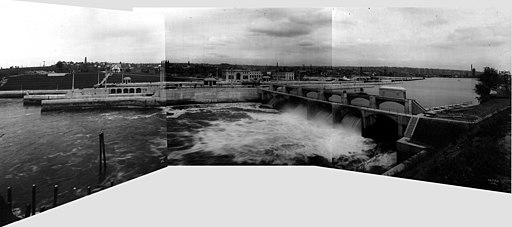
\includegraphics[width = 5 in]{Asahel_Curtis_panorama.jpeg}
\caption{Panorama of Lake Washington Ship Canal, Hiram M Chittenden Locks, Seattle (1917) by Asahel Curtis (public domain). Three overlapping photographs, with different angles of view, are stitched together to form a panorama. This is an example of multi-view analysis.}
\label{fig:image_stitching}
\end{figure}

Whenever two or more images are acquired of the same scene, registration becomes a crucial aspect of image analysis. Common applications include creation of panoramic images (e.g. Figure \ref{fig:image_stitching}), recognition of objects, and video frame alignment. 

Image registration is widely used in modern image capture and processing software, and its applications can be broken down into four broad categories \citep{zitova2003image}:
\begin{itemize}
\item Different viewpoints (multi-view analysis)
\item Different times (multi-temporal analysis)
\item Different sensors (multi-modal analysis)
\item Scene to model registration
\end{itemize}

Early image registration techniques used mechanical methods, e.g. alignment of images on both sides of a strip of film in order to create colour films, a primitive type of multi-modal analysis. In 1963 the first digital image registration technique was published by \citeauthor{roberts1963machine}, enabling machine recognition of objects from photographs \citep{roberts1963machine}. This research developed the techniques of using the total squared error to measure the (dis)similarity between an image and a computer model, and of finding a transformation to minimize this (scene to model registration).

Within medical image registration, early uses concentrated on finding the scale and/or translation required to compare a patient scan to a template image (scene to model registration), e.g. \cite{barber1976digital}, \cite{appledorn1980automated}. As computational power increased, and digital images became the norm, the number and complexity of methods exploded.

%Todo: More pictures of examples of registration

The simplest form of registration is \textit{rigid} registration. This consists of choosing values for six parameters (three for two-dimensional images) to describe the optimal rotation and translation of one (\textit{floating}) image in 3 dimensions, to match it with the other (\textit{reference}) image. The inclusion of further \textit{affine} transformations including scaling, reflection, and shearing adds more flexibility to the registration. In the most general case, a non-linear or \textit{elastic} registration method allows the floating image to be deformed, for example to account for changes due to breathing or the heart beating during scanning.
%Todo: Continue writing classical and recent important literature summary.

This study deals exclusively with multi-modal analysis of biomedical images in two dimensions. However, methods that are designed for multi-view or multi-temporal analysis are also described here, where relevant to the methods that are evaluated. Some of the methods discussed were first published for three-dimensional (volume) data but can be applied also to two-dimensional images. The remainder of this chapter gives an overview of these registration methods, including intensity-based similarity measures such as mutual information, feature-based techniques including the scale-invariant feature transform, structural representation techniques, and deep learning. The details of the two methods evaluated in this study can be found in Chapter \ref{sec:models}.

\section{Intensity-based Similarity Measures}
Intensity-based measures in general compare the intensity at each pixel (or voxel) in the reference image with that at the corresponding pixel in the floating image, under a given transform. In the simplest case, the resulting metric is aggregated globally over all pixels to give a scalar similarity measure. Some methods modify this to account for local variation in contrast or intensity, e.g. to improve performance in the presence of shadows.
\subsection{Sum of Squared Differences}
A simple measure of the dissimilarity between a pair of images is the sum of squared differences (SSD). For images $I$ and $J$, with intensities $I(x)$ and $J(x)$, the SSD is given by
\[
SSD = \sum_{x} (I(x)-J(x))^2,
\]
where the sum is over all overlapping pixels $x$ under a given transform. Since the number of overlapping pixels varies depending on the transform used, the mean squared error (MSE) is normally used instead, i.e.
\[
MSE = \frac{1}{N}\sum_{x} (I(x)-J(x))^2,
\]
for a pair of images overlapping at $N$ pixels. The optimal alignment is then the one that minimizes the MSE. However, this measure is not robust to variations in (for example) illumination, and can be biased by large intensity differences at a few pixels, which may occur due to noise. It is also only applicable to mono-modal image registration.

\subsection{Mutual Information}
\begin{figure}
\centering
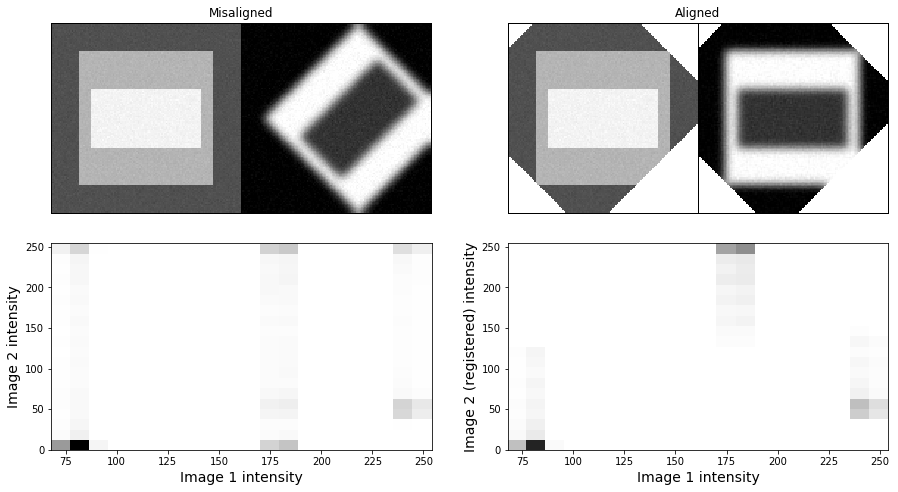
\includegraphics[width = 5 in]{MI_joint_histogram.png}
\caption{Mutual Information histograms for aligned and misaligned images. A pair of artificial images is shown, each containing three intensity values, plus smoothing and noise. On the left, the images are misaligned, and in this case six separate peaks can be seen in the joint histogram of intensity values. The first image has entropy $H_A=3.62$, the second has entropy $H_B=4.36$. The joint entropy when misaligned is $H_{AB}=7.39$, giving mutual information $I(A,B)=H_A+H_B-H_{AB}=0.59$. On the right, the images have been aligned by applying rotation and translation, and pixels that do not overlap are excluded, shown here as white regions. Only three peaks can be seen in the joint histogram, corresponding to the three main intensities in the images. Masking out non-overlapping pixels increases the entropy of the individual images to $H_A'=3.67$, $H_B'=4.82$. The joint entropy however is reduced to $H_{AB}'=7.34$, giving a mutual information score of $I(A,B)'=1.15$.}
\label{fig:MI_histogram}
\end{figure}

The use of mutual information (MI) for image registration was first proposed by \cite{wells1996multi} and \cite{viola1997alignment}, and at the same time by \cite{maes1997multimodality}. MI is a global information theoretic measure which evaluates the amount of information about one image that can be gleaned from another, for a given alignment, and is based purely on the pairs of image intensities at each overlapping position. This does not require there to be a one-to-one or continuous mapping between intensities in the two images, nor any common edges or features. This makes the method particularly suitable for multi-modal image registration. Intuitively, it relies on the assumption that there will be some set of structures that appear similar to each other in one image (self-similarity), that are also self-similar in the other image. The more that this assumption holds true, the more the knowledge of the intensities in one image gives information about the likely intensities in the other image.

The mutual information between a pair of images $A$ and $B$ is calculated as
\begin{equation}
I(A,B) = H_A + H_B - H_{AB},
\label{eq:MI}
\end{equation}
where $H_X$ is the entropy of image $X$. If the image has $L$ intensity levels (e.g. $L=255$ for 8 bit images), appearing with probabilities $p_0, ..., p_{L-1}$, its entropy is defined as
\[
H_X = - \sum_{i = 0}^L p_i \text{log}({p_i}).
\]
The entropy of an individual image is maximal when all possible intensities are equally well represented. An image containing only a single intensity level has the lowest possible entropy.

For pairs of images, the entropy is defined similarly, but using pairs of intensities ($a_j, b_j$) found at corresponding pixels in images $A$ and $B$. There are $L^2$ possible pairs of intensities, and each pair $i$ occurs with some probability $p_i$ in the pair of images. Then the joint entropy is given by
\[
H_{AB} = - \sum_{i = 0}^{L^2} p_i \text{log}({p_i}).
\]

The total image entropies $H_A$ and $H_B$ for the reference and floating images respectively are fixed values, but when calculating the MI of a particular candidate alignment only the overlapping part of the floating image is included. This means that as the proposed registration changes $H_B$ also changes, but in the method proposed by \cite{wells1996multi}, $H_A$ is treated as a constant. It is also possible (e.g. see \cite{maes1997multimodality}) to consider only the overlapping parts of both images, allowing both $H_A$ and $H_B$ to change according to the alignment. This is the approach adopted here when evaluating methods, in Section \ref{sec:evaluation}, and is illustrated in Figure \ref{fig:MI_histogram}.

The calculation of MI uses the relative probabilities of each pair of intensities found in the two images. The probability $p_i$ of a particular intensity value occurring in an image can be estimated empirically as the normalised frequency of observations of that value, and the joint histogram can be constructed similarly. Since the locations in the transformed image are likely to lie in between original pixel co-ordinates, in the simplest implementation the intensity values used in the histogram may be calculated based on their nearest neighbour, or using bilinear or spline interpolation followed by binning. Improved results, particularly if sub-pixel accuracy is desired, may be obtained using partial volume interpolation to update the histogram such that each off-pixel point contributes a weighted amount to the histogram at the intensity values of each of its nearest whole-pixel neighbours \citep{maes1997multimodality}. Alternatively, \cite{viola1997alignment} smoothed the probability estimates by using a window function known as a Parzen Estimator \citep{parzen1962estimation}, calculated as:
\[
p_i \approx \frac{1}{N} \sum_{a_j \in I} R(i - I(a_j)),
\]
where $R(x)$ is a window function, such as a Gaussian density function, that integrates to 1, and $N$ is the number of pixels (or voxels) in image $I$, which has intensity $I(a)$ at pixel $a$.

These histogram modifiers are designed to increase the robustness of the metric to noise, as well as to improve the smoothness of the MI gradient as the transform changes, but also tend to increase the computation time. Another way to reduce the impact of noise is to bin intensity values, e.g. into 32 bins, and this is adopted here (following \cite{gee2003biomedical} and others).

Maximization of mutual information leads to a good alignment in many multi-modal cases, without requiring any \textit{a priori} knowledge of the correspondence between different intensities in the two modalities. For example, \cite{wells1996multi} presented the results of using MI to register 3-dimensional magnetic resonance (MR) images with both computed tomography (CT) and positron-emission tomography (PET) images. 

MI remains a popular and commonly-used measure of image similarity, particularly for multi-modal image alignment. However, it can be difficult to locate the MI maximum, due to the existence of local optima and/or low gradients, particularly when the initial registration is far from the true alignment, and/or in the presence of noise \citep{maes1997multimodality}.

\subsection{Variants of Mutual Information}
Several refinements to mutual information have been published, including Normalized Mutual Information, Adjusted Mutual Information, and Region Mutual Information. These aim to improve the performance of mutual information in various situations.

\cite{studholme1999overlap} introduced \textbf{Normalized Mutual Information} (NMI). This is designed to deal with the case where the size of the region of overlap between two images may change depending on the chosen registration parameters, which can lead to unwanted effects on the mutual information statistic. Instead of calculating the difference between the marginal and joint entropies (as in Equation \ref{eq:MI}), the NMI is given by the ratio:
\begin{equation}
I_N(A,B) = \frac{H_A + H_B}{H_{AB}}.
\label{eq:NMI}
\end{equation}

\textbf{Adjusted Mutual Information} (AMI, \cite{vinh2009information}) takes into account the probability that image intensities are correlated purely by chance, which depends on the number of different intensities and the relative frequencies of each. This has been shown to be preferable to plain mutual information \citep{vinh2009information} but increases the computation time considerably.

\textbf{Region Mutual Information} (RMI, \cite{russakoff2004image}) aims to account for the spatial relations between pixels, rather than treating the entire image as a one-dimensional signal. Instead of calculating marginal and joint entropies on the basis of the intensity at each pixel, the intensities of neighbouring pixels are included (e.g. 8 neighbouring pixels in 2D), leading to a high-dimensional joint distribution (e.g. pairs of 9-dimensional vectors). Using a simplifying assumption based on Principal Components Analysis, the authors show that this can be calculated in similar time to mutual information ($\mathcal{O}(N^2)$ for $N$ pixels). It is more robust than MI when the initial registration error is large.

A number of other variants have been designed for non-rigid registration, including conditional mutual information \citep{loeckx2010nonrigid} and Self-Similarity $\alpha$ MI \citep{rivaz2014self}.

\subsection{Other intensity-based similarity measures}
The negative joint entropy $-H_{AB}$ can also be used on its own as a global measure of similarity for multi-modal images \citep{collignon19953d}, and is improved by supersampling. An efficient implementation can be obtained by binning grey-level values.

\cite{rogelj2003point} developed a Segmentation-Based Point Similarity Measure which first estimates the classes of intensity pairs that are true correspondences, based on the distribution of intensity pairs in the current alignment, and assumes that at the correct alignment the intensity pairs follow a Gaussian distribution around the centres of these classes. This gives a model of the joint intensity distribution which can then be used to assess the quality of the registration.

\subsection{Registration with intensity-based similarity measures}
For each of the above measures of image similarity, the measure itself only provides a metric to evaluate the alignment for a given transform $T$. In order to register a pair of images $A$ and $B$, it is necessary to find the transform $\hat{T}$ that, when applied to $B$, maximises the similarity $S(A, T(B))$ of the two images, i.e. 
\[
\hat{T}=\argmax_T S(A,T(B)).
\]
This is commonly achieved using gradient ascent, but many other optimization techniques have been proposed, such as particle swarm optimization (e.g. \cite{wachowiak2004approach}).


\section{Feature-based Techniques}
One inherent drawback of intensity-based registration methods such as most of those described above is that they treat the images as a one-dimensional array of intensity values, and make no use of information about the locality or neighbourhood in which each value occurs. Feature-based techniques approach the problem from a different angle, looking instead for common structures such as corners within an image, and then trying to find a correspondence between the sets of features found in each image. This can facilitate comparison of images which differ in (for example) lighting conditions or contrast, because the intensities are not used directly.

In general the first step is to identify keypoints within each image, and describe them in a way that can be compared across different scales, orientations, and/or imaging conditions. Then these keypoints must be matched between the two images, and from this, an appropriate transform can be inferred. Feature-based techniques are also commonly used for image recognition.

Some of the most commonly used feature-based methods are outlined in this section.
\subsection{Harris corner detector}
\begin{figure}
\centering
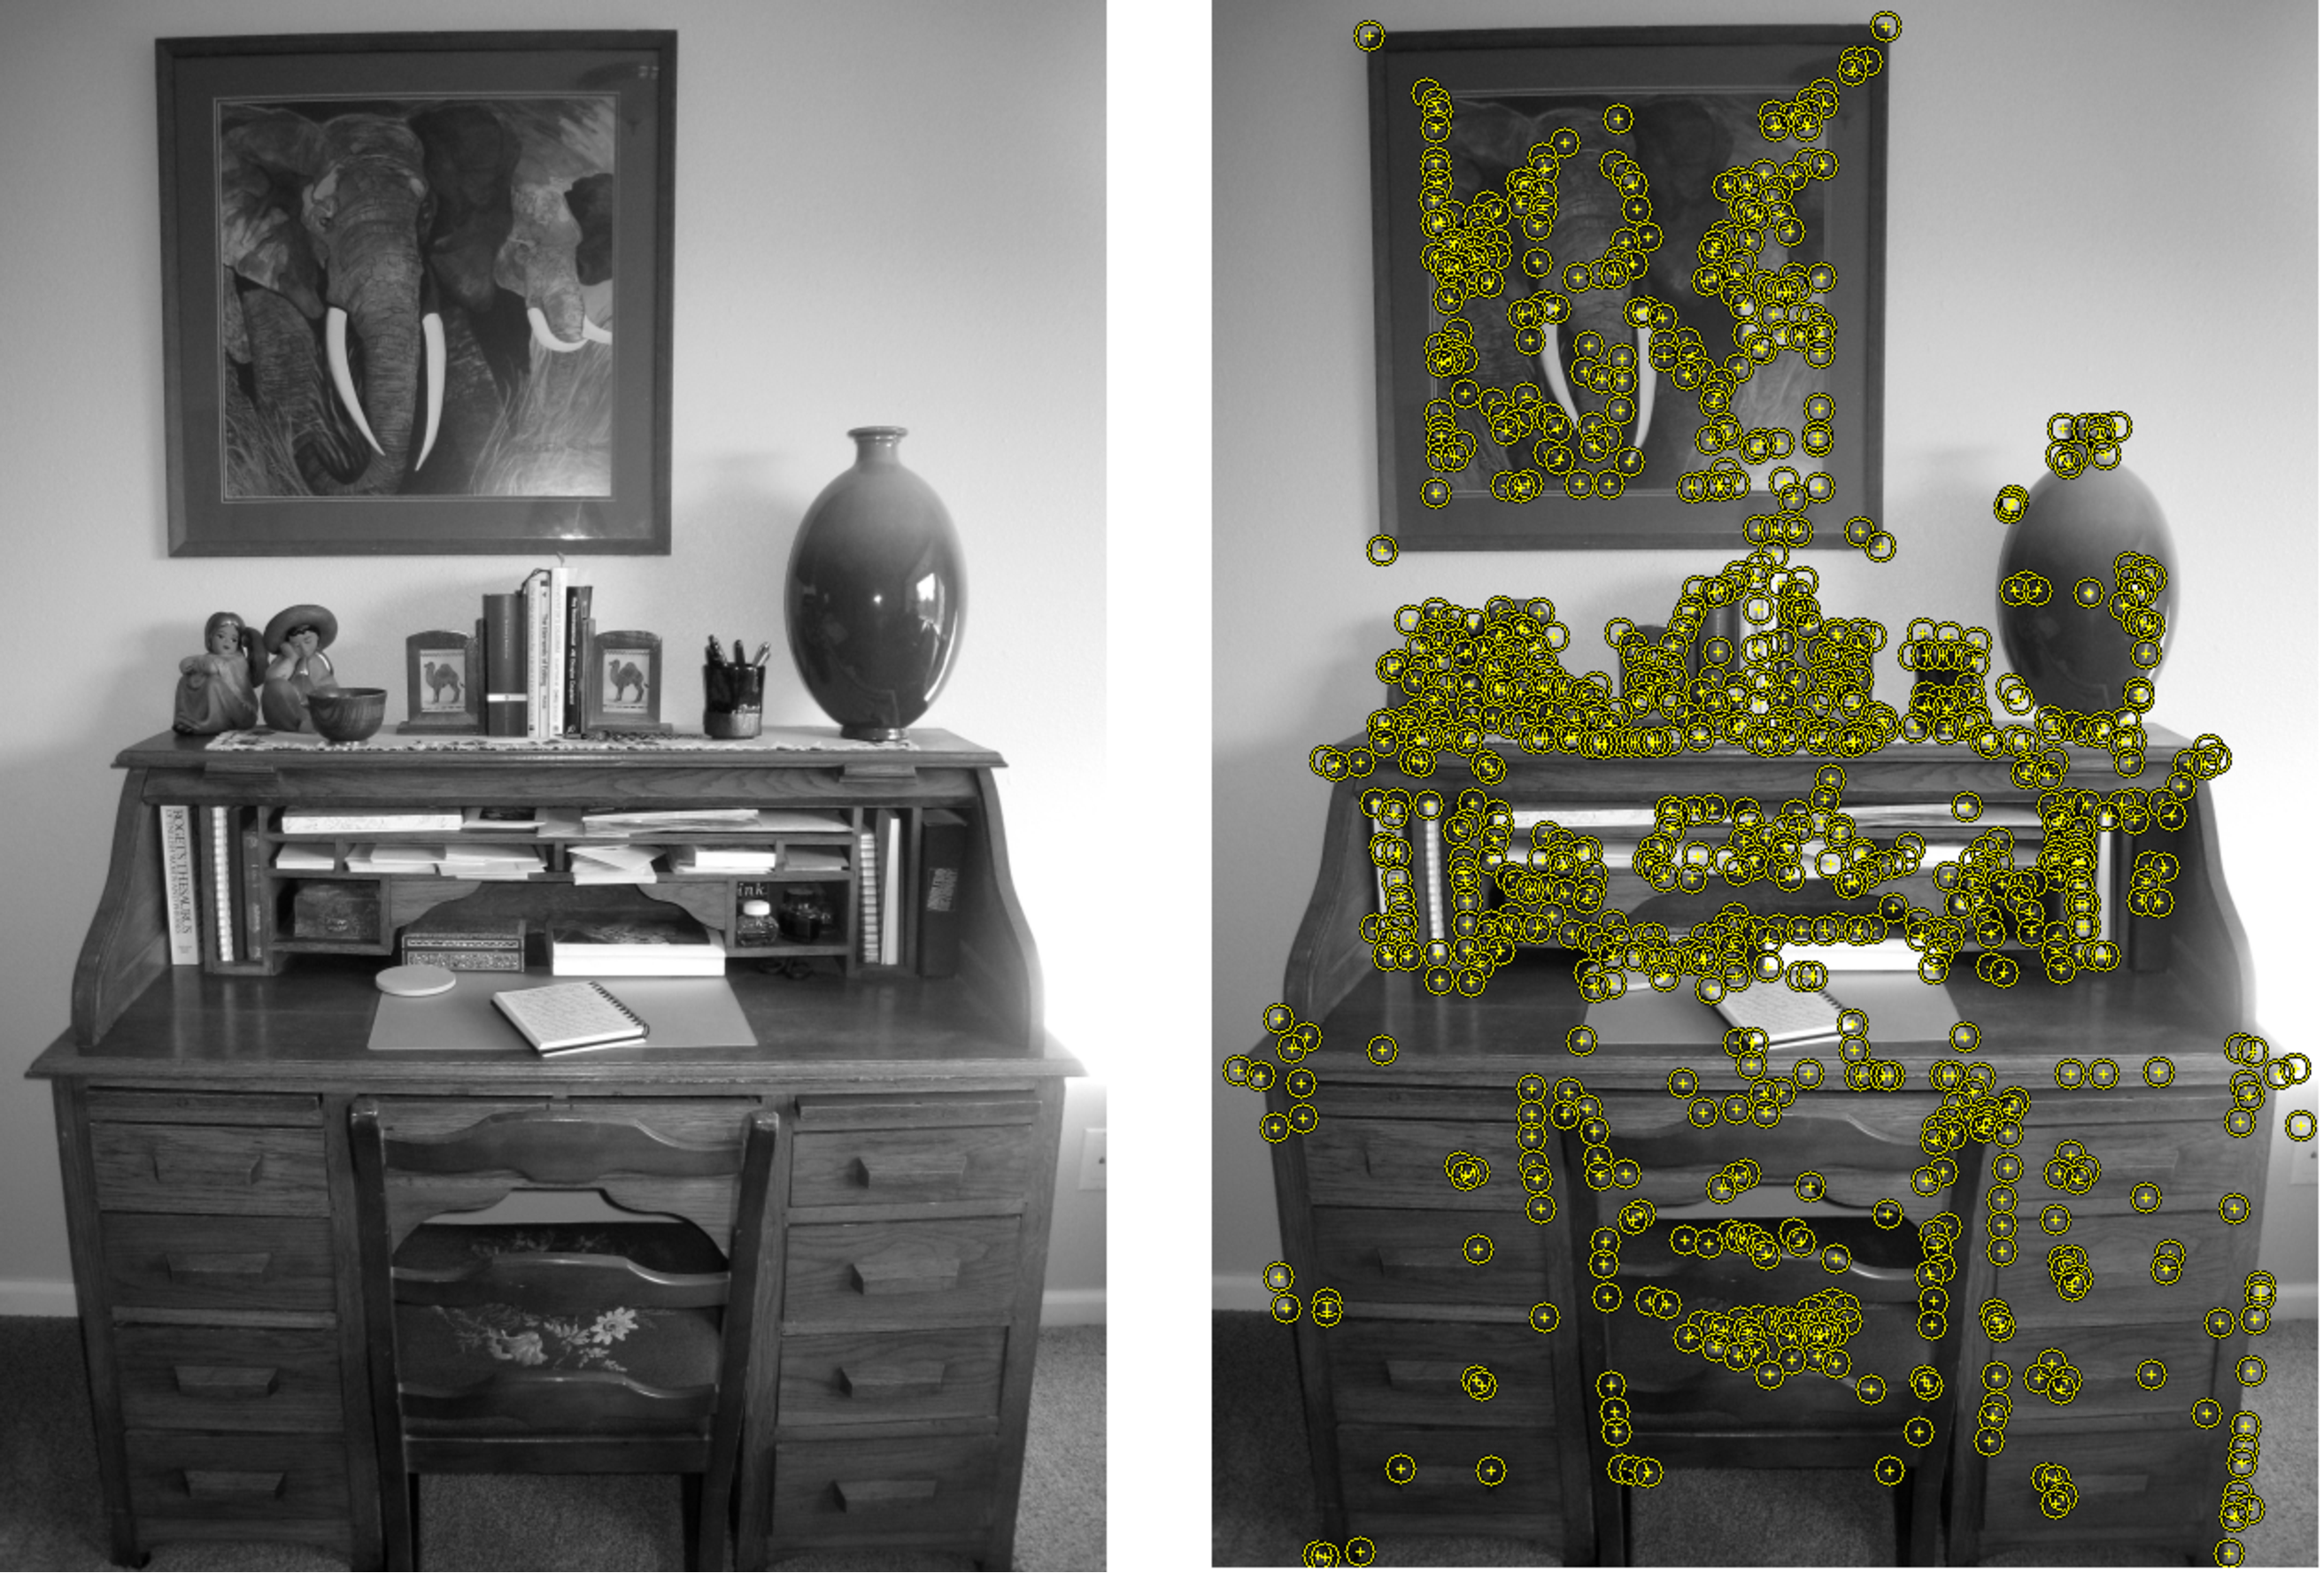
\includegraphics[width = 5.5 in]{Writing_Desk_with_Harris_Detector.pdf}
\caption{An example showing features detected with the Harris corner detector. Image by  Dvortygirl \texttt{https://commons.wikimedia.org/w/index.php?curid=11497200}.}
\label{fig:harris_features}
\end{figure}
An early feature-detection method was developed for tracking objects in the presence of camera motion, by \cite{harris1988combined}. This method identifies corners as locations where the image intensity gradient is high in multiple directions, at a specified scale. The Harris corner detector, and variants upon it, are the basis of many feature-detection methods. An example of the features that would detected by the Harris corner detector is shown in Figure \ref{fig:harris_features}.

\subsection{Scale-Invariant Feature Transform}
A popular method in medical image registration in general is the scale-invariant feature transform (SIFT) \citep{lowe2004distinctive}. This uses a multi-scale Difference of Gaussians (DoG) approach to locate and describe keypoints in an image
%, which can then be compared to a large database of features for object recognition
. The feature descriptors, consisting of 128 values for each keypoint, are invariant to orientation and scale. This property is important for image registration, as it allows keypoints in one image to be matched with those in another image, which may be at a different rotation, scale etc. 
%Then the transform which maps the keypoints most accurately from one image to the other, provides the optimal image registration.

\subsection{Features from Accelerated Segment Test (FAST)}
\begin{figure}
\centering
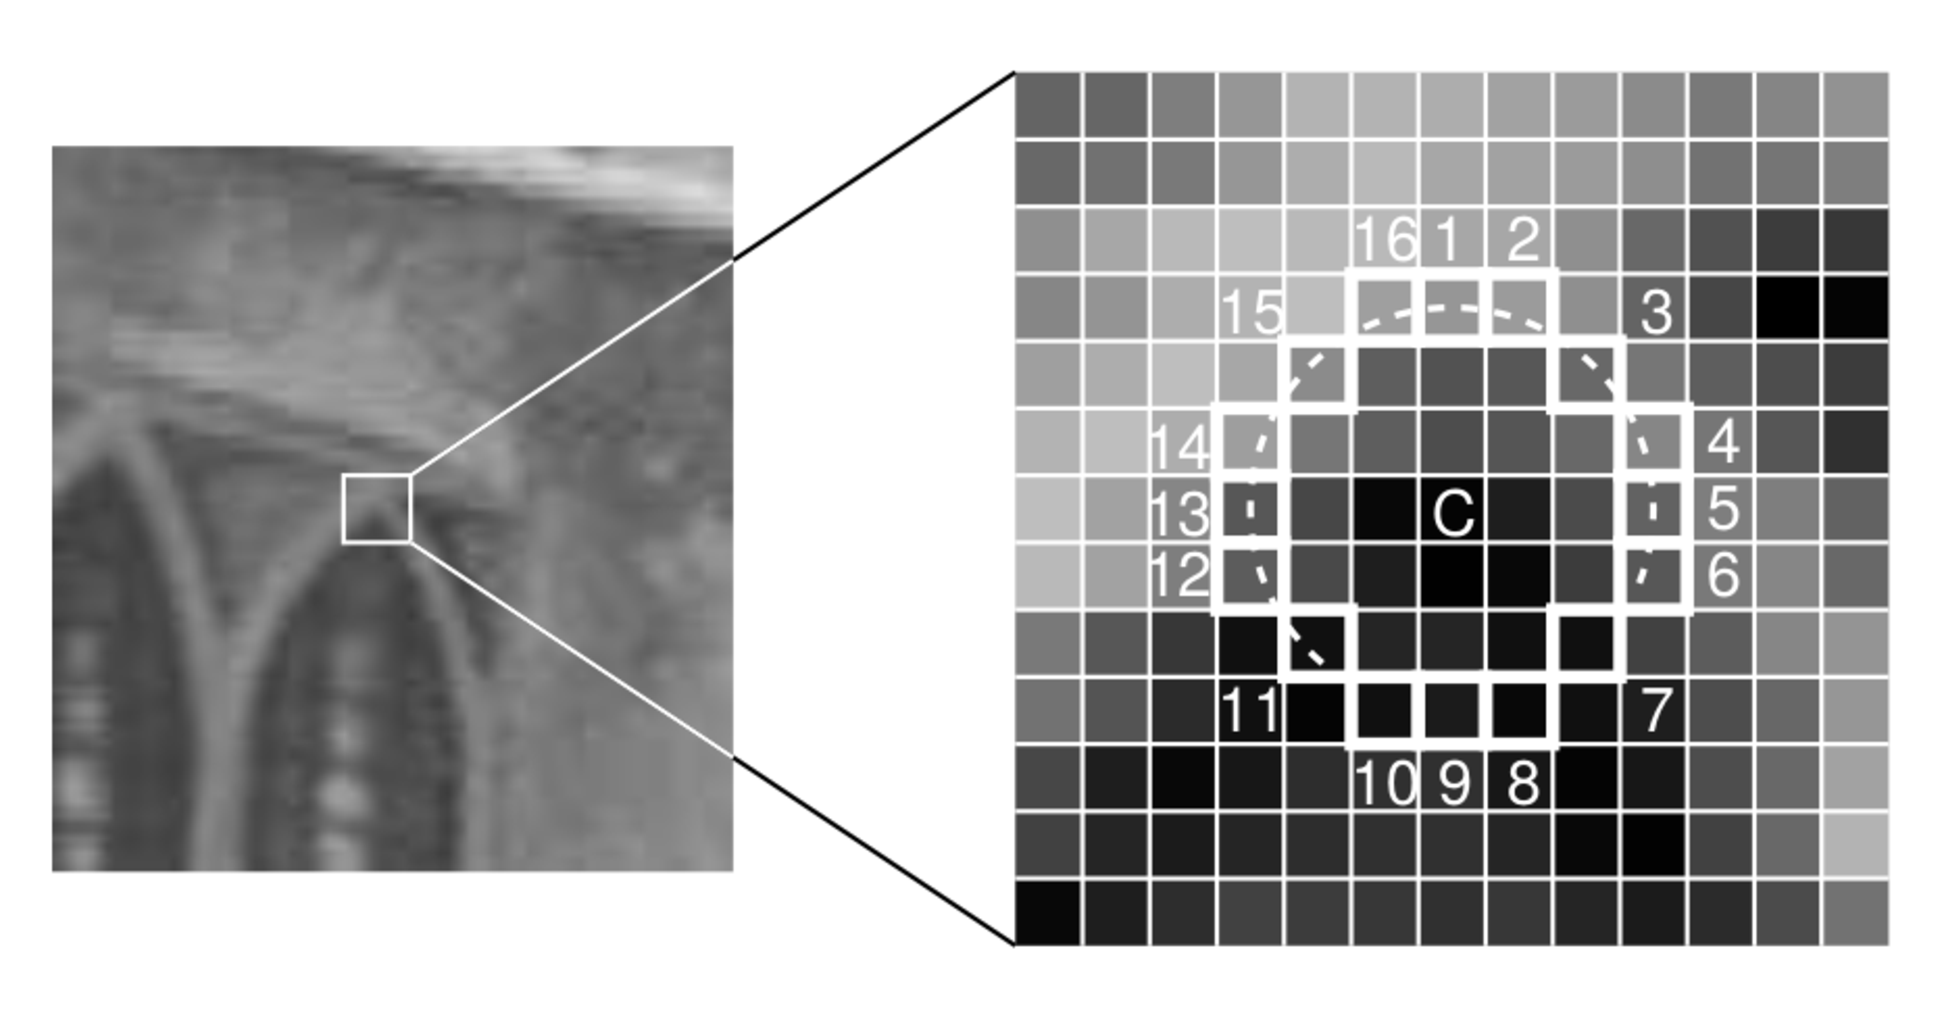
\includegraphics[width=5.5in]{Rosten_Corner_Segment_Test.pdf}
\caption{Segment Test for corner detection, illustration by \cite{rosten2005fusing}. The central pixel $C$ is detected as a corner because, within a circle of 16 pixels centered on $C$, 12 adjacent pixels are all brighter than $C$ by an amount greater than or equal to the threshold $t$.}
\label{fig:rosten}
\end{figure}

The application of supervised learning allowed \cite{rosten2006machine} to develop a feature detector which operates much faster than SIFT without sacrificing accuracy. Their detector is based on the Segment Test introduced in their earlier work \citep{rosten2005fusing}. This defines a corner as a location $p$ where, in a circle of 16 points centred around $p$, at least $n$ contiguous points are brighter than (or darker than) the central point by some intensity threshold $t$. This is illustrated in Figure \ref{fig:rosten}.

Applying the full segment test directly to each pixel proved too costly for real-time video processing. Although significant speed improvements can be made by first testing just 4 pixels from the circle of 16, and only continuing if these values indicate a potential corner, this restricts the possible values of $n$ to 12 or greater, thereby excluding any shallow corners from being detected. Instead, the authors trained a decision tree model, by using the full segment test to define the desired outputs for a set of training images. The tree can then be applied to unseen images to predict where the corner features are located. A score function can be applied to each of these detected points, to filter out the weaker signals.

Once trained, the decision tree is extremely fast and can be used to detect features in video streams in real time. As well as speed advantages the method was shown to outperform several other methods, including the Harris corner detector and methods based on the Difference of Gaussians (as used by SIFT).
%Todo: write more about SIFT and FAST and others

%
%\subsection{Oriented FAST and Rotated BRIEF (ORB)}
%\cite{rublee2011orb} also developed a faster alternative to SIFT, known as ORB. This modifies the BRIEF feature descriptor \citep{calonder2010brief} to improve its performance in the presence of rotation, and modifies the FAST keypoint finder \citep{rosten2006machine} to add a measure of the orientation of keypoints. Their results showed that ORB can match or outperform SIFT in many applications, particularly in the presence of noise and/or orientation differences.

\subsection{Registration with feature-based techniques}
The above techniques extract a set of feature locations from each image that is to be aligned, and give each location a feature description. It is then necessary to find a correspondence between these features, and then finally to calculate the transform $T$ that best explains the feature pairing. Since many hundreds of keypoints may be found in each image, matching them is not a trivial task. A brute-force approach, in which each keypoint descriptor in one set is compared to every keypoint descriptor in the other set, is highly computationally intensive. Instead, the K-Nearest Neighbour (KNN) algorithm is often used to determine the best match for each keypoint in one image. When each keypoint in one image has been allocated a corresponding location in the other image, then Random Sample Consensus (RANSAC, \cite{fischler1981random}) can be used to determine what transform $T$ best maps one image to the other.
%TODO: this is still short - write something about KNN.

\section{Structural representation techniques}
\label{sec:backgroundSR}
Structural representation methods attempt to overcome the problems inherent in multi-modal registration, by transforming both images into a representation which encapsulates the structural information of the image, independent of the modality. These structural representations can then be registered using mono-modal registration techniques. Some of the most important structural representation techniques are described below. Methods evaluated in this study are described in more detail in Chapter \ref{sec:models}.

\subsection{Local binary and local derivative patterns}
Local binary patterns (LBPs), developed by \cite{ojala2002multiresolution}, are a popular and efficient technique in image classification and registration, %TODO citation needed
in which the intensity value of each pixel is compared to its $P$ neighbours, equally spaced around a circle of radius $R$ around the central pixel. The result is thresholded at zero to give a $P$-bit binary representation of the intensity pattern for that pixel. This can be seen as an encoding of the sign of the first order derivative in each of $P$ directions. By varying the radius $R$, structure can be extracted at different scales. A measure of image similarity can be obtained by comparing the binary representations of the two images. This measure is invariant to monotonic differences in the intensity values of the two images, such as luminance or contrast differences.

\begin{figure}
\centering
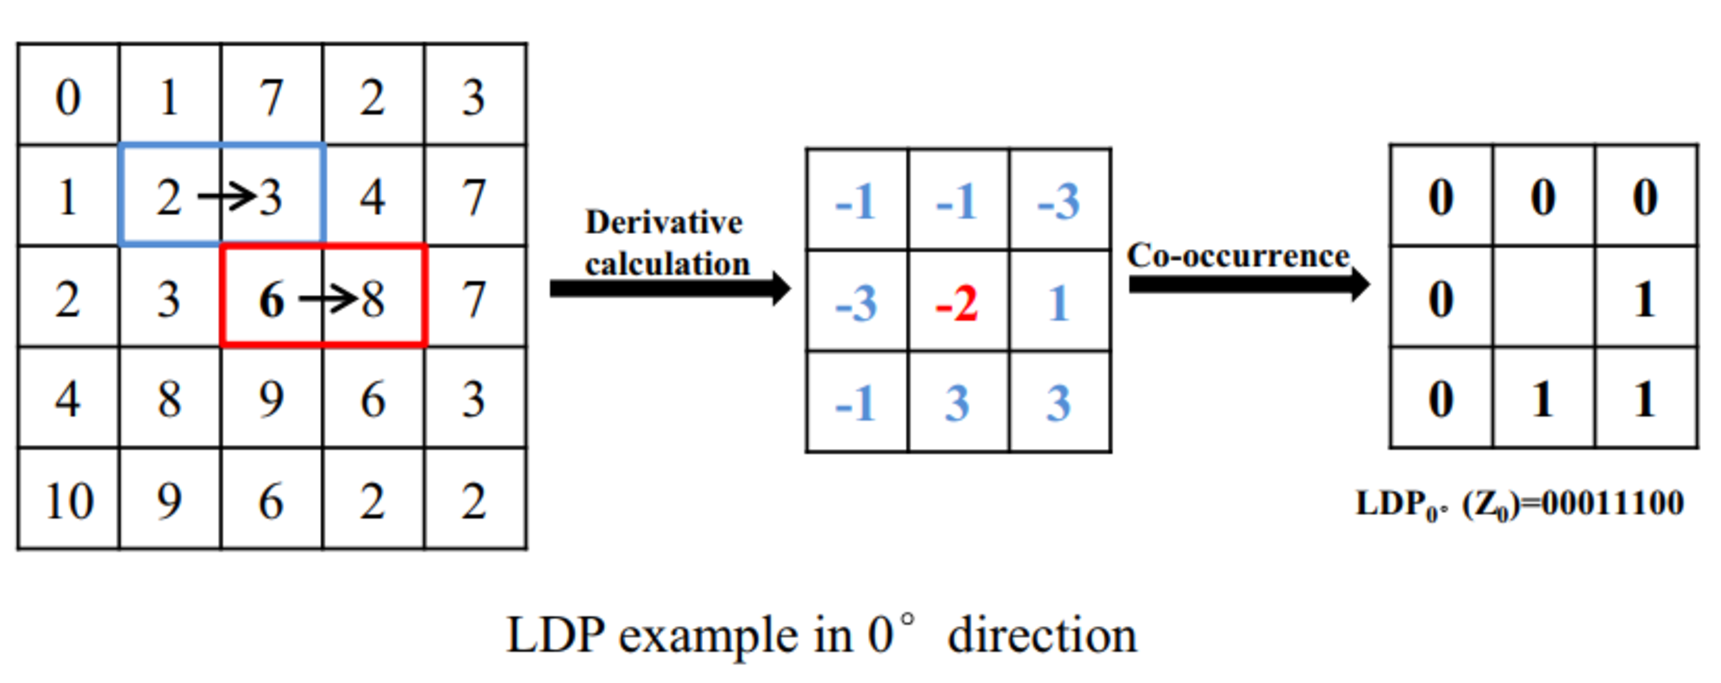
\includegraphics[width=5.5in]{LDPexample_jiang.pdf}
\caption{Calculation of the Local Derivative Pattern, illustration by \cite{jiang2017fast}. For each pixel in a $3\times 3$ patch (the centre of the region shown), the derivative in the $x$ direction, i.e. the difference between its intensity and that of its right-hand neighbour, is calculated. Pixels whose derivative have the same sign as the derivative at the central pixel are encoded as zeros. Pixels with the opposite sign are encoded as ones. The eight results are concatenated into a binary string representation. The equivalent calculation of the Local Binary Pattern would encode the sign of the difference between the central pixel and each neighbour, giving LBP($Z_0$)=11101001.}
\label{fig:LDP}
\end{figure}
%todo extend the LDP diagram to show the LBP as well

Local derivative patterns (LDPs) generalize the idea of LBPs, to define an encoding of the second order (and higher) derivatives. 

To calculate the second order LDP for a pixel $i$, the first order derivative in a particular direction $d$ is found for each pixel in a patch centred on $i$, by taking the difference in intensity between that pixel and its immediate neighbour in the $d$ direction. The sign of each of these differences is compared with the sign of the derivative for the central pixel, to create a binary string (8 bit in the case of a $3 \times 3$ patch). The calculation is illustrated for 0 degrees in Figure \ref{fig:LDP}. This is then repeated for a number of directions, usually covering 0, 45, 90, and 135 degrees. The concatenation of these four 8-bit binary strings gives a 32-bit representation of the signs of the second order partial derivatives at pixel $i$.

It is possible to extend LDPs to higher order derivatives but this increases their sensitivity to noise \citep{jiang2017fast}.

\subsection{Modality-independent neighbourhood descriptors}

Another effective structural representation method, Modality-independent neighbourhood descriptors (MIND), published by \cite{heinrich2012mind}, defines a distance metric comparing each point $x$ in an image with a set of other pixels $R$ within the surrounding region, not only comparing the individual pixel intensities but incorporating information about the local neighbourhood of each pixel. The two-dimensional version of the method is outlined here and would form an excellent avenue for further research on the dataset used in this study.
 
The distance measure $D$ for a pair of pixels ($x$ and $r$) within a single image is based on equally-sized image patches centred on each point, and calculates the sum of squared differences between the intensities at each pixel $p$ in those patches:
\[
D(x,r) = \sum_p (I(x+p)-I(r+p))^2,
\]
where $I(x)$ is the image intensity at point $x$ and $x+p$ indicates the position of $x$, offset by $p$. The patch size can be configured for the particular application. 

They use the exponential of the distance measure $D$, divided by a local variance measure $V$ (equal to the average distance metric between the current pixel and its four immediate neighbours) and normalized, calculated for some set of nearby pixels $r \in R$, as a descriptive vector for each pixel:

\[
\text{MIND}(x,r) = \frac{1}{n}\text{exp}\left( - \frac{D(x, r)}{V(x)} \right), r \in R.
\]

\begin{figure}
\centering
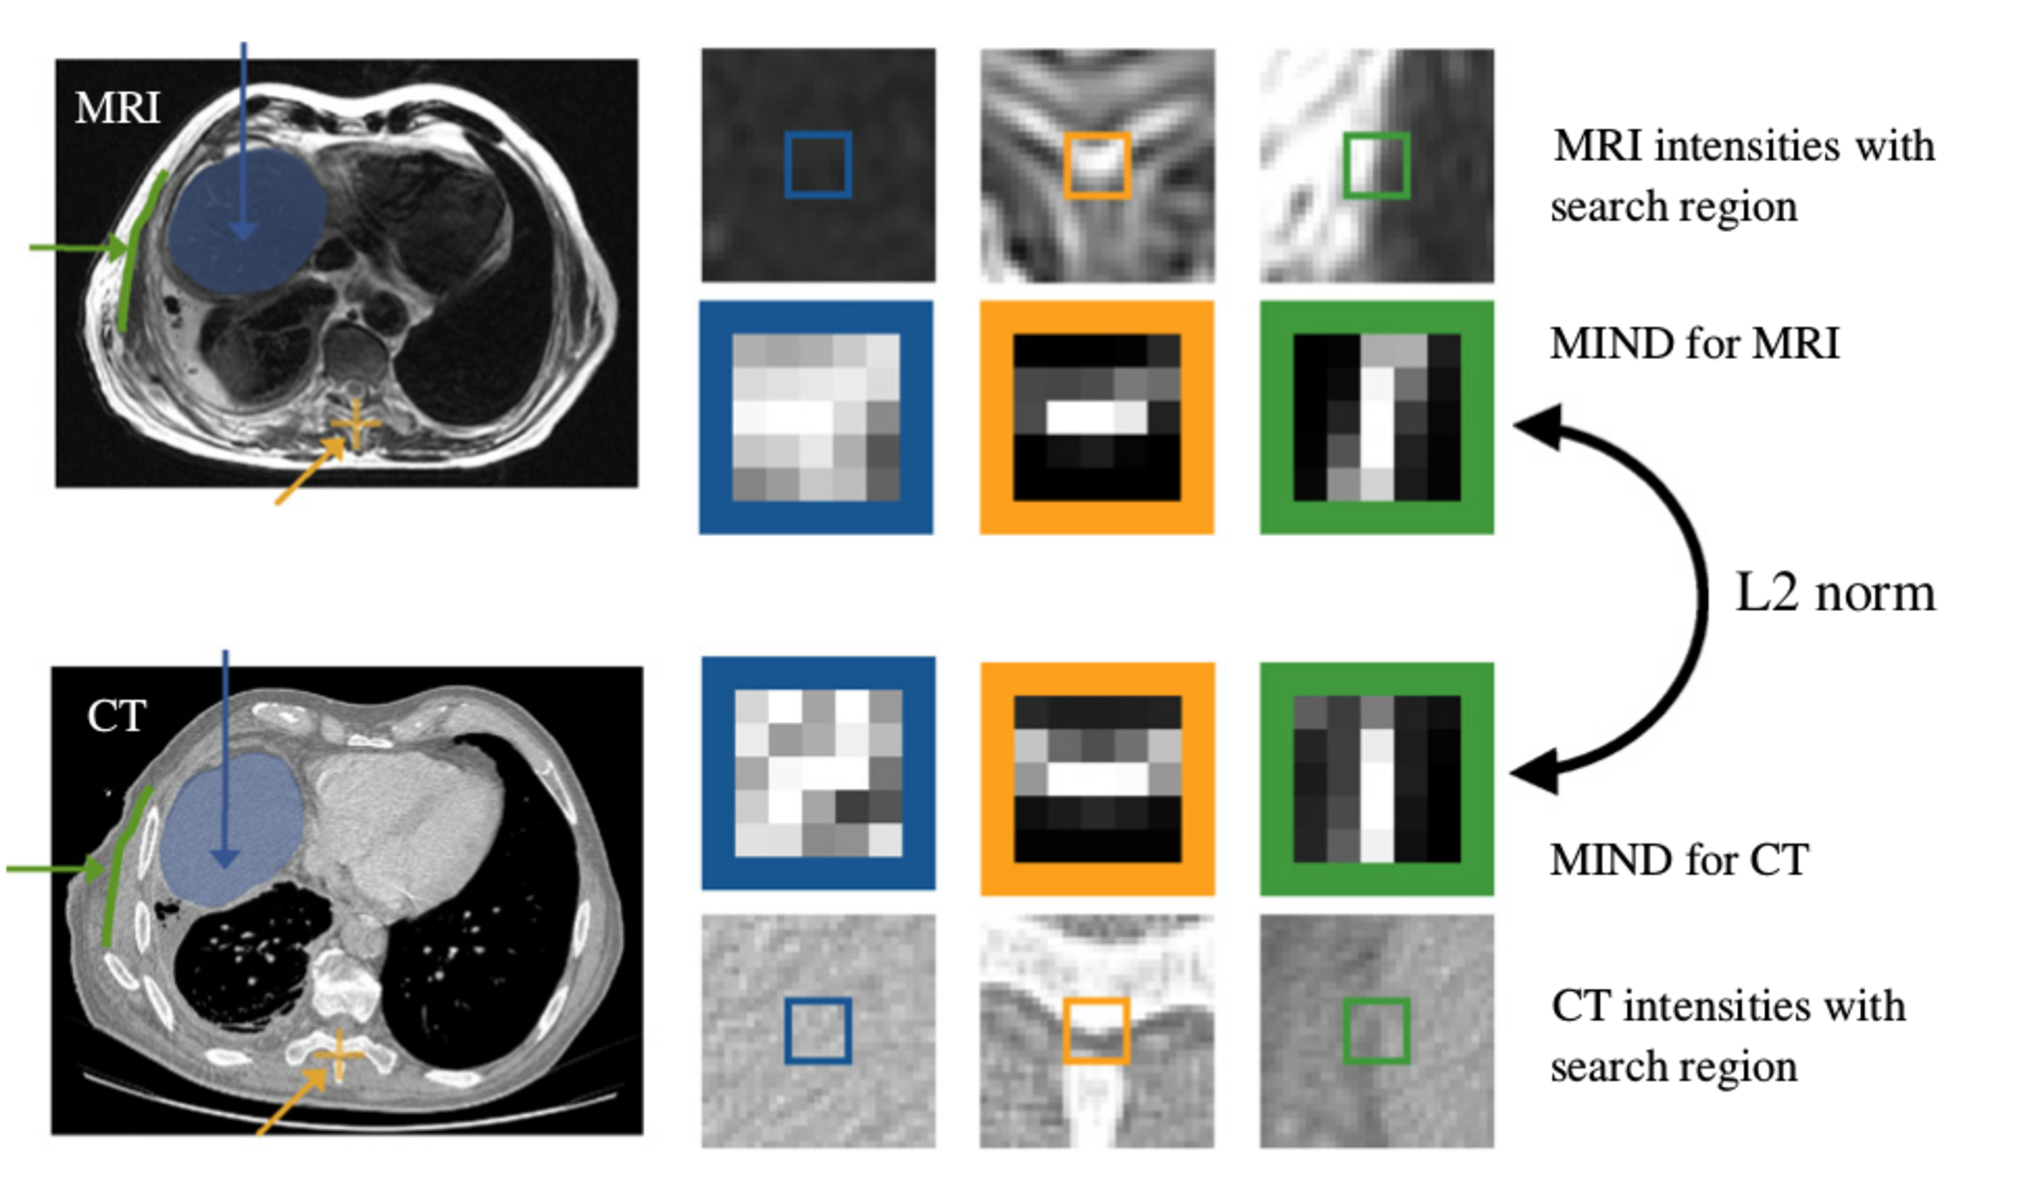
\includegraphics[width=5.5in]{mind_orig.pdf}
\caption{Modality-independent neighbourhood descriptors, illustration by \cite{heinrich2012mind}. Three pixels are indicated on the images, located in different regions of interest. For each of these pixels, the MIND descriptor based on a 5x5 region is shown. Homogeneous regions, corner points, and boundaries all have distinctive appearances which are independent of the image modality.}
\label{fig:MIND}
\end{figure}

This descriptor is then compared between the two images, and the (dis-)similarity of the images at a given pixel is defined as the average of the squared differences between the elements of the corresponding vectors (see Figure \ref{fig:MIND}). The transform that minimizes this metric is chosen as the optimal alignment of the images.

They calculate the metric efficiently using convolutions, but it needs to be calculated for each pair of pixels within some search range of each other, which makes it computationally expensive. The search region can however be reduced by only sampling neighbours along the 8 compass point directions (instead of the 5x5 dense region illustrated in Figure \ref{fig:MIND}). For computational efficiency the authors suggest quantizing the MIND descriptor down to 4 bits, then for sufficiently small search region $R$, every possible value of the descriptor (i.e. $16|R|$ values) can be precomputed into a lookup table. The MIND descriptor is robust to noise and contrast differences and excellent results were demonstrated on the alignment of CT images with MRI in three dimensions, including for deformable registration.


%\subsection{Laplacian eigenmaps}

\section{Deep learning for image registration}
In recent years, a number of deep learning techniques have been developed for image registration. One approach is to use deep learning to identify features, e.g. the convolutional neural network proposed by \cite{dosovitskiy2015discriminative}. Other models directly estimate the transform $T$ that aligns a pair of images, based on a large training dataset (e.g. \cite{detone2016deep}).

%TODO write more
Deep learning approaches usually offer good performance, once an initial training phase is completed, and are likely to be the future of image registration as more data becomes publicly available and as methods evolve. They will not be covered in this study but would make a good avenue for future work with this particular dataset.

\chapter{Models}
\label{sec:models}
This study focuses on structural representations, which offer perhaps the best hope for aligning images with modalities that differ greatly. %TODO citation?

Two models are compared and contrasted here, with baseline results given by Mutual Information. The first, PCANet-based structural representation (PSR), was developed by \cite{zhu2018pcanet} and uses Principal Components Analysis to determine the filter coefficients in a small convolutional neural network (CNN). The outputs of the CNN are then used to create a representation incorporating multi-level structural information. This process is described in more detail in Section \ref{sec:model1} below.

The second model, published by \cite{jiang2017fast}, uses Local Derivative Patterns to extract structure from the images. More information is given in Section \ref{sec:model2}.

Both models are chosen for their excellent results in the registration of multi-modal medical images.

\section{Model 1: PCANet-based Structural Representation}
\label{sec:model1}
The first model to be evaluated, by \cite{zhu2018pcanet}, embeds the technique of principal components analysis (PCA) within a convolutional neural network (CNN) to create a PCANet-based structural representation (PSR). It builds on the work of \cite{chan2015pcanet}, using PCA to create feature maps for image classification within a deep learning framework. This model has been shown to be effective in the registration of various different types of magnetic resonance (MR) images, (PD, T1 and T2), including in the presence of noise, and registration of computed tomography and MR images, outperforming MIND and NMI amongst other models.

The filter weights in the CNN are trained separately for each modality of interest, and the trained model can then be used to output structural representations of any images of that modality. The overall architecture of the model is illustrated in Figure \ref{fig:PSR}.

\begin{figure}
\centering
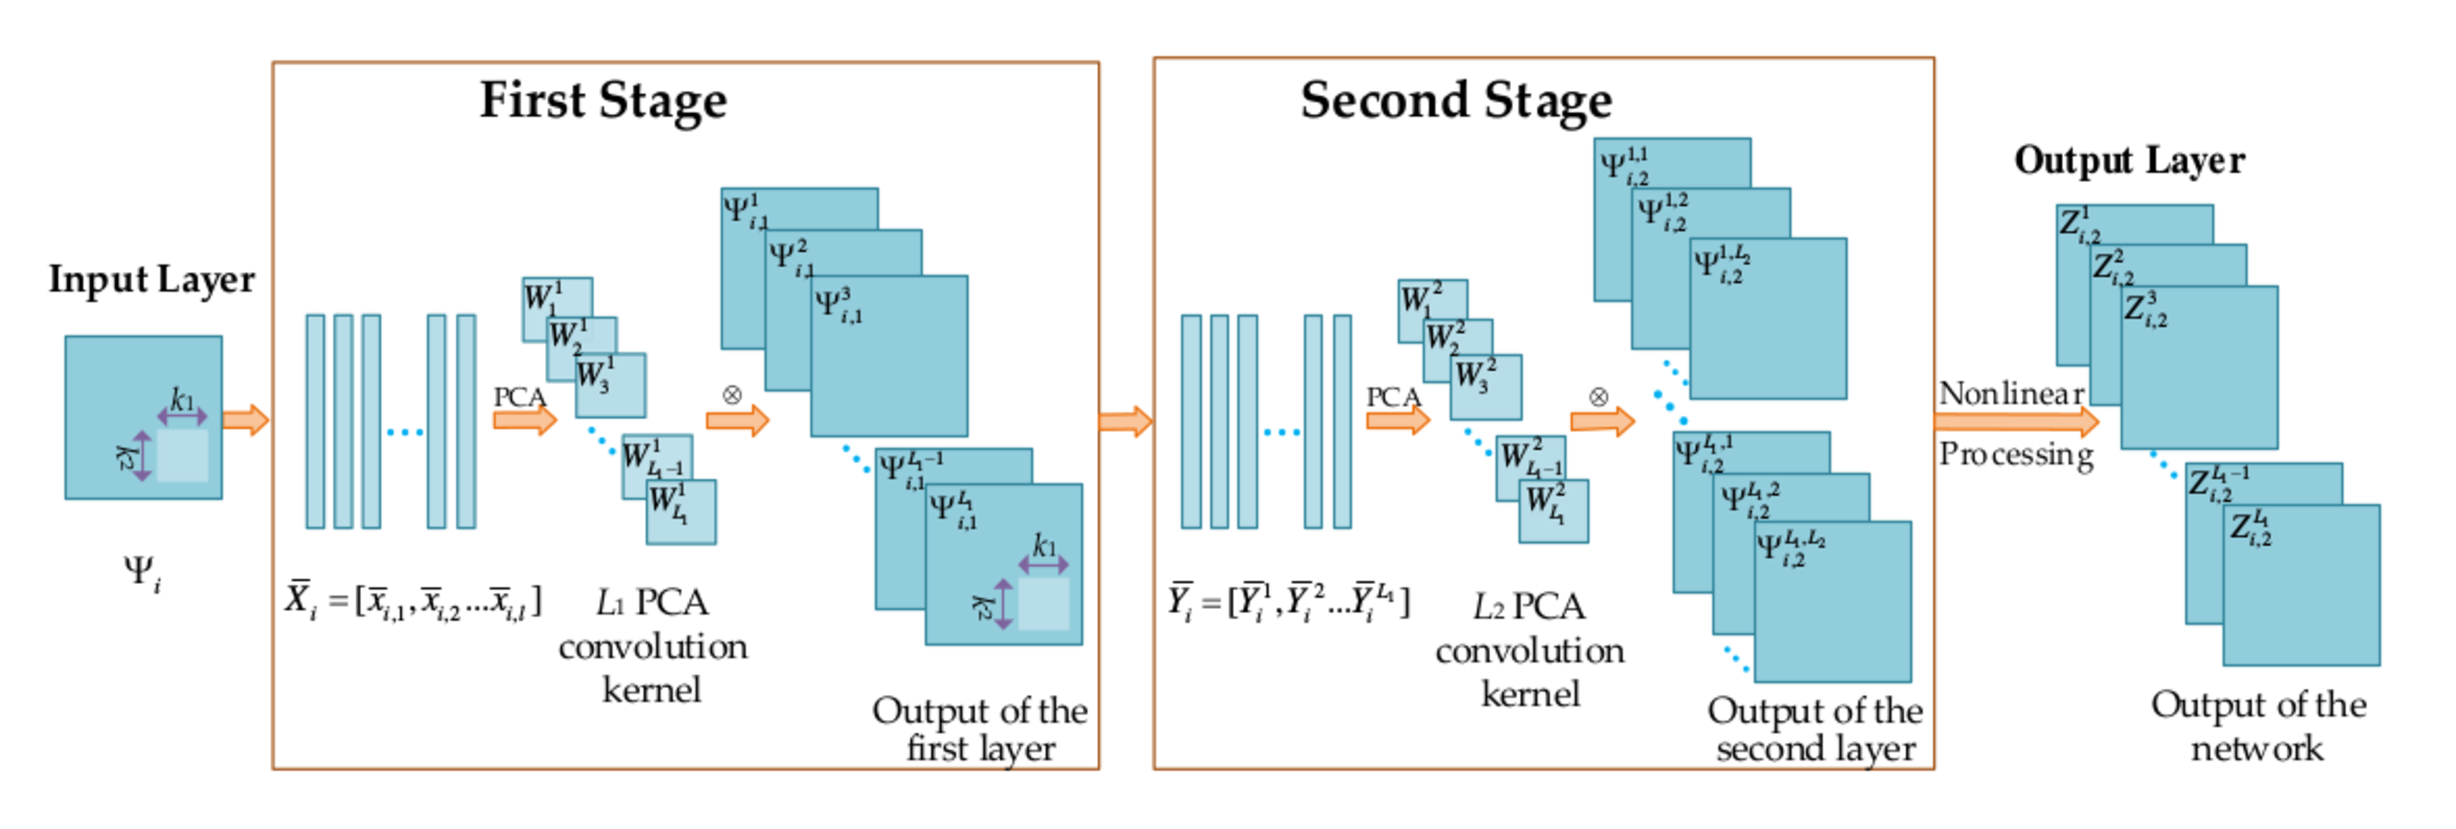
\includegraphics[width=5.5in]{PSR_architecture.pdf}
\caption{Architecture of the PCANet-based Structural Representation CNN, illustration by \cite{zhu2018pcanet}. In the first stage, a number of input training images are converted into a set of overlapping $3\times 3$ patches, and each patch is treated as a vector of image intensity values. The principal components of these vectors are used as filter weights in a convolutional layer. The resulting feature maps are passed as inputs to the second stage, and processed similarly.}
\label{fig:PSR}
\end{figure}

There are several tuneable parameters within the model. In this study the size of the filters was fixed at $3 \times 3$, the number of filters in each layer was fixed as 8, and the number of layers was fixed as 2. The parameter $\alpha$ was set to 0.005. All of these choices follow the recommendations given by the original authors \citep{zhu2018pcanet}. Exploratory experiments with different filter sizes resulted in no improvements in results. Since the method used to construct feature maps from filter outputs in the second layer (described below) weights each subsequent filter half as much as the previous one, the addition of extra filters (at least in the second layer) is also not expected to have a significant impact on the results.

\subsubsection{Calculating the filter weights}
To determine the filter weights for a given modality, a set of 100 randomly chosen training images are used. For each pixel $j$ in a training image $\Psi_i$, the image intensities in a $3 \times 3$ patch centered on that pixel are collected into a vector $x_{i,j}$. Pixels on the boundary of the image are excluded. For each patch, the patch mean is subtracted to give a zero-centred vector $\bar{x}_{i,j}$. All of these patch vectors, for all of the training images, are collated as the columns of a matrix $\bar{X}$. 

Principal components analysis is then employed to determine the $L_1$ principal eigenvectors of this matrix, i.e. those relating to the $L_1$ largest eigenvalues, where $L_1=8$ is the number of filters in the first layer of the network. These eigenvectors are each rearranged into a $3 \times 3$ matrix of filter weights, such that the filter weights are in the same order as the image patches were arranged.

The second layer of the CNN consists of $L_2=8$ filters, and takes as its inputs the $L_1$ outputs of the first layer, for each of the training images. Every $3 \times 3$ patch in every input is collected and a similar principal components analysis is performed to determine the filter weights for the second layer.

This single application of a two-layer convolutional network completes the training phase of the model; no gradient-based training method (such as backprop) is required. This means that the training phase is fast to compute, although performing PCA on such large collections of vectors is highly memory-intensive. Structural representations are then created by passing images through this network and combining the outputs from the filters and layers into a single output image or feature map.

\subsubsection{Combining the outputs}
\label{sec:featuremaps}
The CNN described above treats each output from the first layer as a separate input to the second layer, leading to $L_1 \times L_2$ feature map outputs for each image after layer 2. These are first combined into $L_1$ feature maps through a sigmoid activation function and a weighted sum. The layer 2 output for image $i$ is given by 
\[
Z_{i}^{j} = \sum_{k=1}^{L_2} 2^{8-k}(\sigma(|\Psi_i^{j,k}|)-0.5),
\]
where $\Psi_i^{j,k}$ is the output obtained from applying the $k$th filter in layer 2 to the output $\Psi_i^j$ of filter $j$ in layer 1 for image $i$, and $\sigma(x)$ is the sigmoid function $\sigma(x) = 1/(1+e^{-\alpha x})$ and $\alpha=0.005$. This has the effect of weighting the layer 2 outputs heavily by their PCA rank, i.e. the output from the first layer 2 filter has twice as much impact as that of the second, which has twice the impact of the third filter and so on.

Having reduced the number of outputs to $L_1$ for each layer, these outputs are then combined into two structural representations, one for each layer, to capture multi-level information. For each layer, a single feature map per original input image is constructed from the $L_1$ outputs by summing the squares of the values in each output:
\[
F_1 = \frac{1}{L_1^2}\sum_{j=1}^{L_1}(\Psi^j)^2;
\]
\[
F_2 = \frac{1}{L_1^2}\sum_{j=1}^{L_1}(Z^j)^2.
\]

The information from the two layers is then finally combined into a single output image:
\[
\text{PSR} = \text{exp}(-\frac{F_1}{h_1})\text{exp}(-\frac{F_2}{h_2}).
\]
The parameters $h_1$ and $h_2$ are calculated at each pixel based on the local variation in the image.

Further details and motivation for this model can be found in \cite{zhu2018pcanet}. The model was implemented in Python using code published by \citeauthor{takeshi2019pcanet} \footnote{https://github.com/IshitaTakeshi/PCANet} as a basis.

\section{Model 2: Discriminative Local Derivative Patterns}
\label{sec:model2}
In this model, second order partial derivatives are utilized to characterize the local structure of an image at each pixel as a vector. This set of vectors forms a modality-independent representation of the image, allowing the similarity between two images to be efficiently estimated on the basis of the Hamming distance between the vector representations. The authors \citep{jiang2017fast} describe the Discriminative Local Derivative Patterns (dLDP) model for 3-dimensional images; here it is presented only in 2D.

As well as excellent results in the alignment of different MRI modalities, and CT with MRI, this method was shown to be effective in the alignment of Ultrasound with MRI volumes, a very challenging multi-modal task.

\subsubsection{LDP and dLDP}
Local Derivative Patterns (LDP), illustrated above in Figure \ref{fig:LDP}, were first introduced by \cite{zhang2009local}, encoding the derivatives within a neighbourhood or patch centred on each pixel of an image. They can be thought of as a generalization of Local Binary Patterns \citep{ojala2002multiresolution}, which encode the sign of the first order derivative in each direction. 

The model evaluated here, proposed by \cite{jiang2017fast}, is based on the second order LDP described above in Section \ref{sec:backgroundSR}, which encodes the commonality of direction between the first order derivative at the central pixel and that at its neighbouring pixels, allowing higher-level structural features such as turning points to be identified. This is particularly important for multi-modal image registration because changes in the direction of the gradient are more likely to be preserved between modalities than the gradient itself. However, a drawback of this descriptor is that, in regions where intensity increases continuously in a given direction (no turning points in the gradient), the resulting binary vector will contain all zeros. With high-resolution images this can occur in a large proportion of pixels, leading to a lack of information in the descriptor and difficulty finding the optimal registration. The authors therefore propose discriminative LDPs (dLDPs), which compare the partial derivative in one direction at the central pixel with that in a (set of) different directions at neighbouring pixels. This is illustrated in Figure \ref{fig:dLDP}.

\begin{figure}
\centering
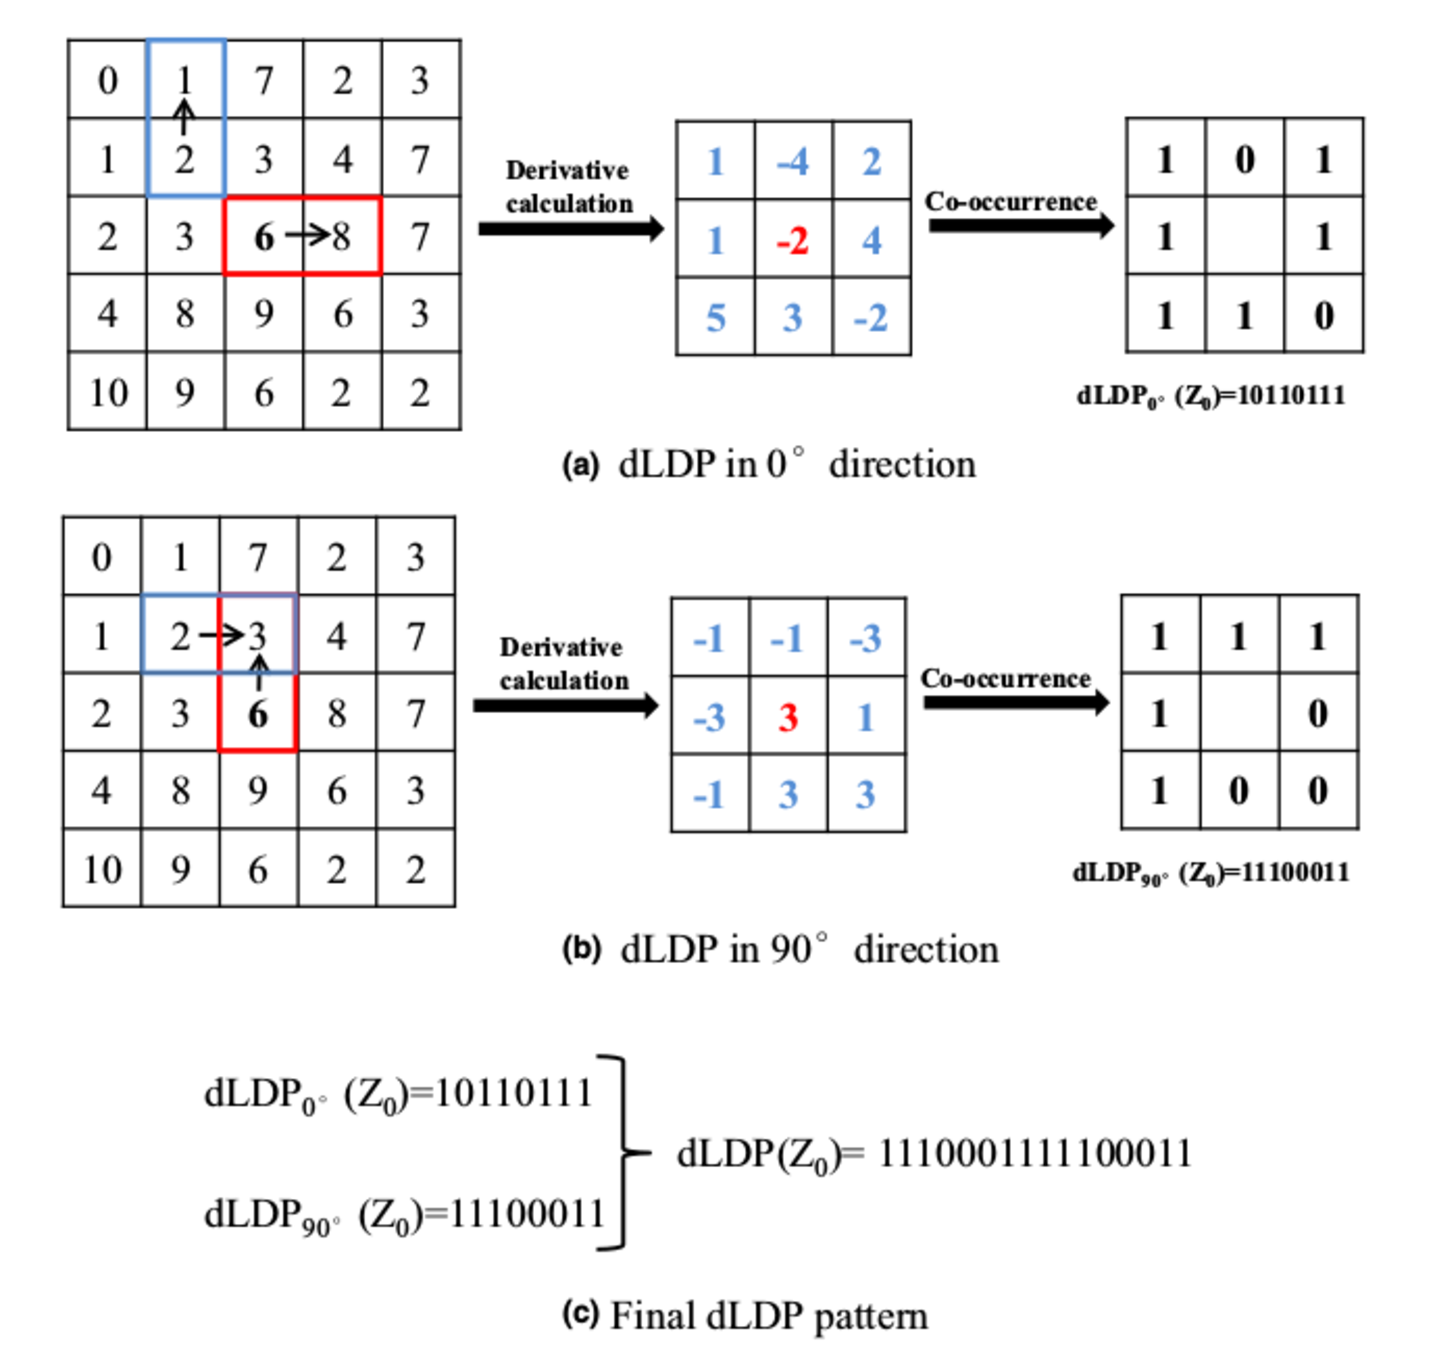
\includegraphics[width=5in]{dLDP_jiang.pdf}
\caption{Calculation of the Discriminative Local Derivative Pattern, illustration by \cite{jiang2017fast}. In step (a), for each pixel in a $3\times 3$ patch (the centre of the region shown), the derivative in the $y$ ($90^{\circ}$) direction, i.e. the difference between its intensity and that of its directly above neighbour, is calculated. For the central pixel, the derivative in the $x$ ($0^{\circ}$) direction is calculated. Pixels whose $y$ derivative have the same sign as the $x$ derivative at the central pixel are encoded as zeros. Pixels with the opposite sign are encoded as ones. The eight results are concatenated into a binary string representation, reading clockwise from the top left. In step (b), this is repeated with the derivative directions swapped. The outputs from steps (a) and (b) are combined in step (c) to give the final 16 bit dLDP pattern. Note that the use of both ($x$, $y$) and ($y$, $x$) pairs is only for illustrative purposes.}
\label{fig:dLDP}
\end{figure}

The published method is designed for three-dimensional image data, and the authors show that it is sufficient to use the derivatives in the x, y, and z directions, omitting any intermediate directions. They use the three direction pairs (x,y), (x,z) and (y,z) to construct the dLDP. The information encoded by the direction pair (y,x) would be very similar to that encoded by (x,y) so the reverse pairs are omitted. This is in contrast to the two-dimensional illustration reproduced here in Figure \ref{fig:dLDP} where the dLDP is constructed from the (x,y) and (y,x) pairs, presumably for illustrative purposes. In this study, two alternative interpretations of the dLDP model in two dimensions are compared, an eight bit dLDP using only the (x,y) direction pair, and a 48 bit dLDP using the six direction pairs ($0^{\circ}$, $45^{\circ}$), ($0^{\circ}$, $90^{\circ}$), ($0^{\circ}$, $135^{\circ}$), ($45^{\circ}$, $90^{\circ}$), ($45^{\circ}$, $135^{\circ}$), ($90^{\circ}$, $135^{\circ}$). These four directions are chosen following the original LDP model \citep{zhang2009local}.

\begin{figure}
\centering
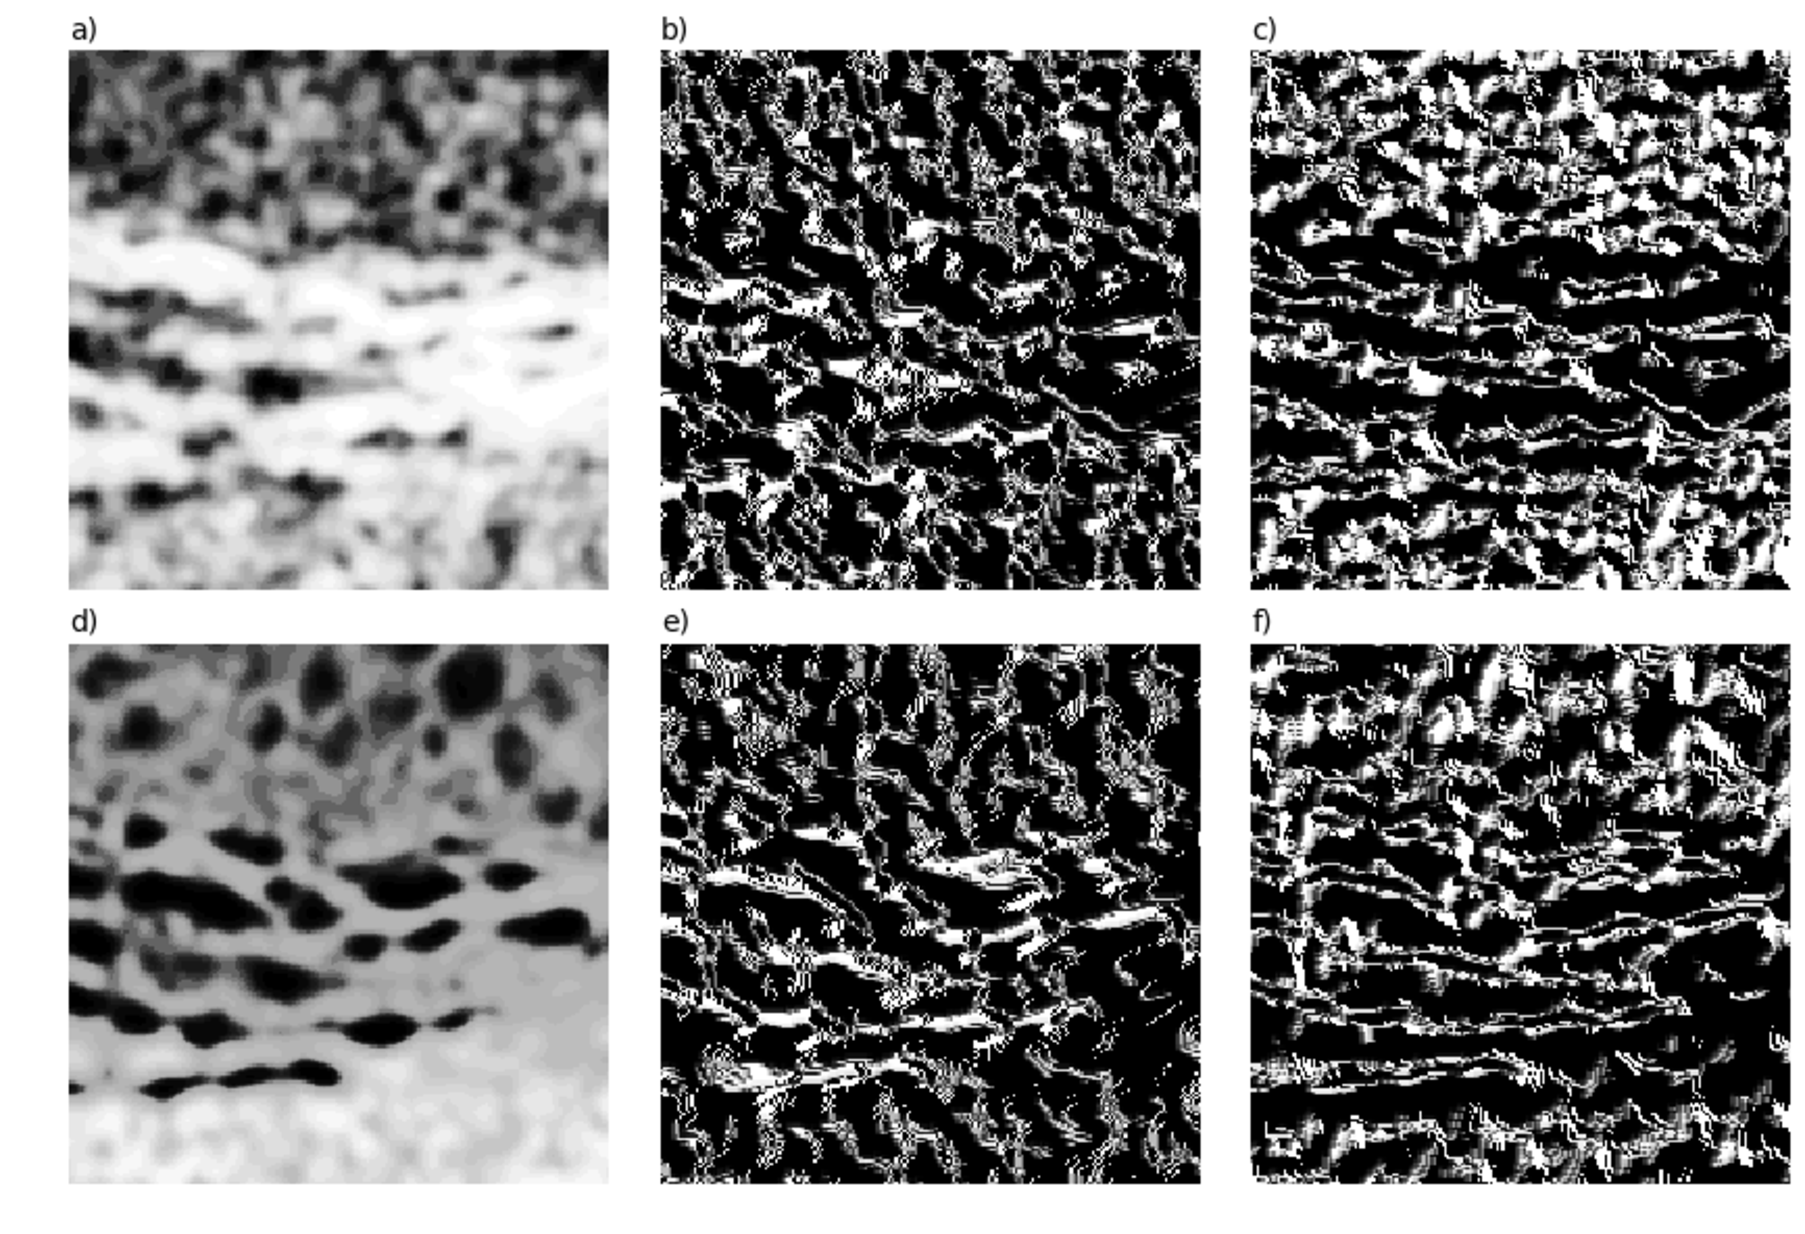
\includegraphics[width=5.5in]{LDP_visualization_zoomin.pdf}
\caption{Illustration of a Discriminative Local Derivative Pattern descriptor. Image (a) shows part of an SHG image after smoothing, histogram equalization and quantization into 32 intensity bins. Image (b) shows the dLDP descriptor for this region for the ($0^{\circ}$, $90^{\circ}$) direction pair. Image (c) shows the dLDP descriptor for the ($45^{\circ}$, $135^{\circ}$) direction pair. Only a small part of the region is shown here, to better visualize the level of detail within the representations. Images (d) to (f) are equivalent images for the TPEF image of the same sub-region.}
\label{fig:dLDP_vis}
\end{figure}
The resulting 48-bit dLDP structural representation is illustrated for one region in Figure \ref{fig:dLDP_vis}. For each direction pair the output is an 8-bit binary vector for each pixel. This can be visualized by interpreting it as an integer between 0 and 255 and showing the result as an image (this method of visualization is also used in \cite{jiang2017fast}). Two of the six direction pairs are illustrated: ($0^{\circ}$, $90^{\circ}$) and ($45^{\circ}$, $135^{\circ}$). In this visualization method, the higher-position bits are emphasised (probably only the first 3 or 4 bits can be distinguished by eye), but it should be noted that when these descriptors are used as a similarity measure (see below), all bits are given equal weighting.

\subsubsection{Similarity measure between representations}
A measure of the similarity of two images can then be obtained by calculating the total Hamming distance between their dLDP representations. In this study, the Hamming distance is normalized by dividing by the number of overlapping pixels. This is not proposed by the original authors but it is clear that for our dataset, the total Hamming distance would be biased towards transforms with minimal overlap. An alternative would be to adjust the Hamming distance to equal half the number of bits used in the descriptor, for each non-overlapping pixel. 

The optimal alignment is then the one which minimizes this normalized Hamming distance.


\chapter{Data}
\label{sec:data}

A set of images of skin tissue samples was provided by our collaborators from the Center for Microscopy - Microanalysis and Information Processing, Polytechnic University of Bucharest. The data collection process is described below. In total the dataset consists of 400 regions of interest taken from 35 different skin samples. These have been categorised as `Healthy', `Dysplastic', and `Malignant' but all three categories are treated together in this study.
%TODO: check numbers

\section{Data collection}
The following information about the data collection procedure is adapted from a description provided by our collaborators.

From each histological block, two consecutive tissue sections are sliced. One is left unstained for Multiphoton Microscopy (MPM) imaging and the other is Haemotoxylin and Eosin (H\&E) stained and imaged with brightfield microscopy (for ground-truth pathology assessment by a trained pathologists). For the H\&E stained slides large image mosaics are assembled. The smaller regions which are imaged with MPM are marked on these mosaics (of the stained slide).  

The two slices are next to each other and only a few nm thick. Most of structures visible in one slice are visible in the other slice as well, but slight changes of shape are expected.

The imaged regions lie at the dermal-epidermal junction (DEJ), a region of high importance in tumor genesis and because the region can potentially be examined with in-vivo MPM imaging in xz directions (it is not very deep, hence accessible to xz MPM).

The unstained slide is imaged using Second Harmonic Generation (SHG) microscopy and Two Photon Excitation Fluorescence (TPEF) microscopy. The TPEF imaging is done for two compounds, Flavin Adenine Dinucleotide (FAD) and Nicotinamide adenine dinucleotide (NADH). Each MPM imaging (SHG, TPEF-FAD, TPEF-NADH) is performed three times, with three different incident polarization angles, spaced 60 degrees apart. A Ti:Sapphire laser tuned at 860 nm ($\sim$ 120 mW power before the microscope) is used for excitation. 
\begin{itemize}
\item For SHG a bandpass filter (425-435 nm) is used.
\item For TPEF (NADH) a bandpass filter 440-490 nm is used.
\item For TPEF (FAD) a bandpass filter 510-600 nm is used.
\end{itemize}

\section{Pre-processing of data}
The above data collection process resulted in 9 MPM images for each region, i.e. three incident polarization angles for each of the three MPM modalities. A single output image for each of these three modalities is then obtained by averaging the image intensities from the three polarization angles. The two TPEF images (NADH and FAD) are further combined to a single TPEF image by taking the mean.

Our collaborators also provided us with processed MPM images, which are colour images composed from the SHG image as the blue channel and the averaged TPEF image as the red channel. These processed images were manually enhanced by adjusting the contrast and gamma correction. Since the gamma and contrast corrections were not known the images were re-processed for this study (omitting the adjustments) and a greyscale (luminance) version was also created using standard RGB conversion parameters: $0.2125*R + 0.0721*B + 0.7154*G$. There is no green channel in this instance.

Finally, our collaborators kindly performed manual alignments for 100 regions of interest to give us a baseline against which to evaluate our methods, providing us with a set of aligned brightfield images. 

\subsection{Histogram equalization}
\label{sec:histeq}
\begin{figure}
\centering
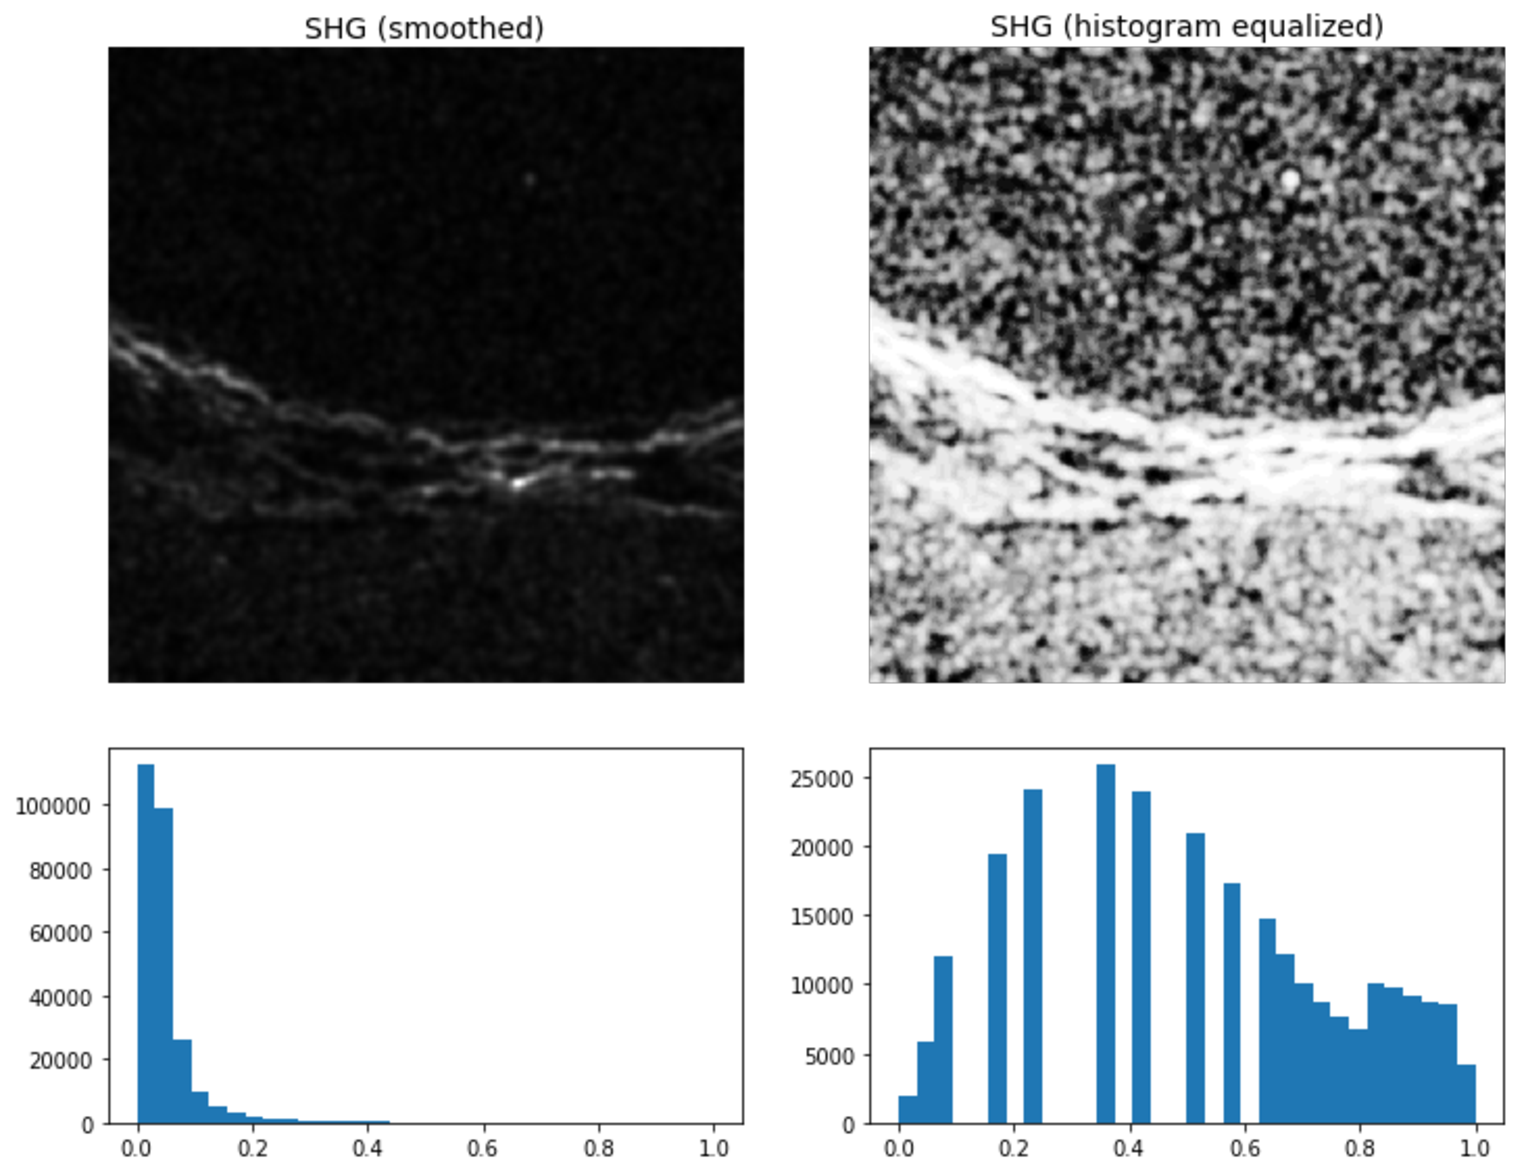
\includegraphics[width = 5.5 in]{histogram_equalization.pdf}
\caption{Histogram Equalization shifts image intensities to better take advantage of the full spectrum. The left-hand column shows an SHG image which has been smoothed, and the corresponding histogram of intensity values. The values are heavily concentrated in the lower end of the spectrum. The right-hand column shows the same region after histogram equalization, and the corresponding histogram of intensities. The contrast in the image is much higher, and the intensity values are more spread out.}
\label{fig:hist_equalization}
\end{figure}
A further data pre-processing step which is evaluated in several of the experiments in this study is histogram equalization. This increases the contrast of an image, potentially improving the descriptive power of various image similarity measures.

For an image $I(x)$ containing $L$ discrete intensity levels, the intensities in the histogram equalized version $I'(x)$ are given by
\begin{equation}
I'(x) = \text{floor}((L-1)\sum_{i=0}^{I(x)}p_i),
\end{equation}
where $p_i$ is the frequency of intensity $i$ in the original image (i.e. the proportion of pixels $x$ for which $I(x)=i$).

This technique shifts the intensity values found in an image such that they are better spread out over the full range of possible intensity values, as illustrated in Figure \ref{fig:hist_equalization}.

\section{Selection of data}
\begin{figure}
\centering
\subfloat[]{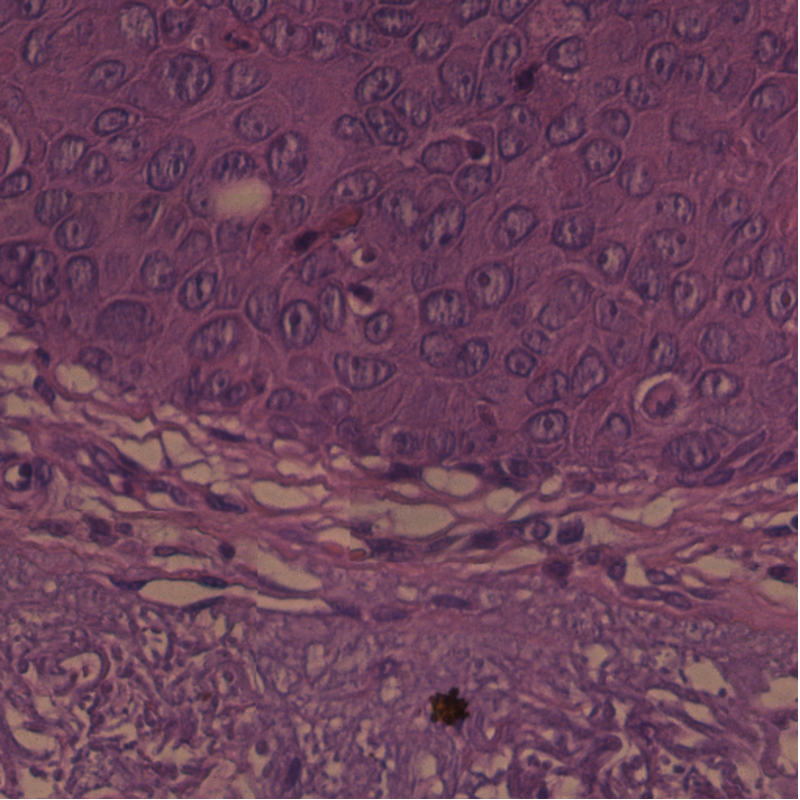
\includegraphics[width = 2.2 in]{aligned_brightfield_148185_11.pdf}} \
\subfloat[]{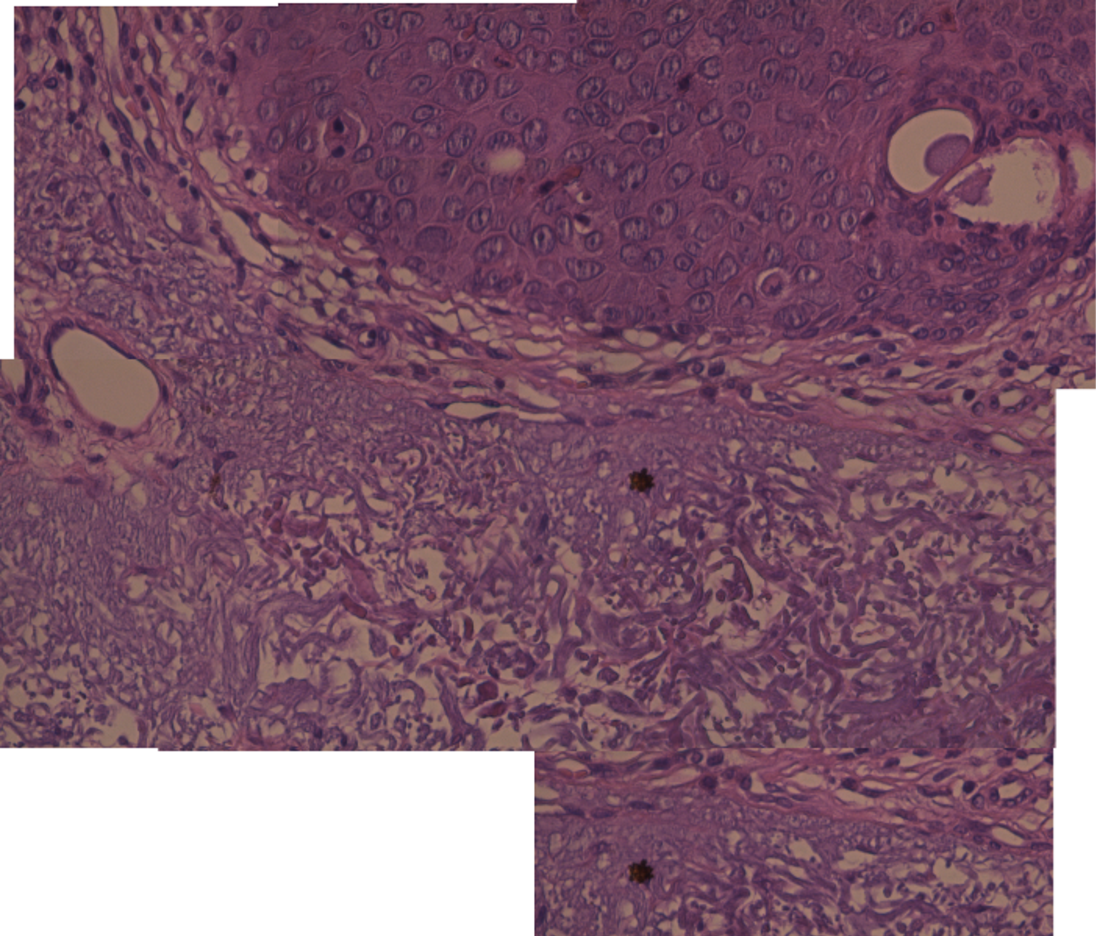
\includegraphics[height = 2.2 in]{brightfield_minimosaic_148185_11.pdf}} \\
\subfloat[]{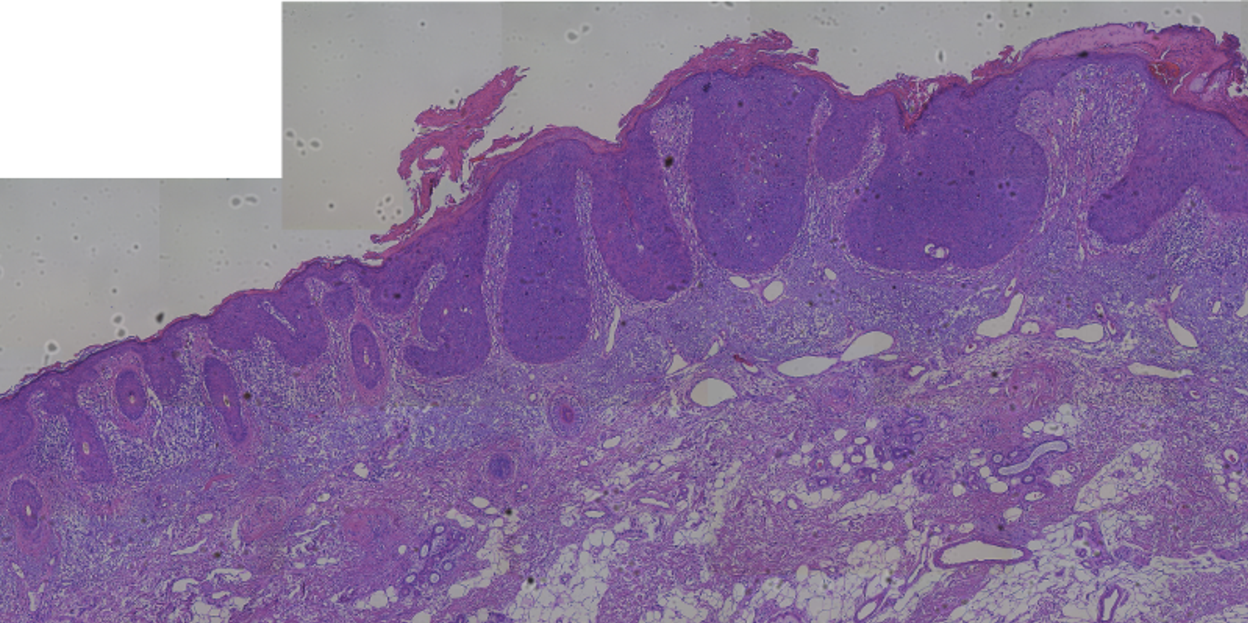
\includegraphics[width = 4.5 in]{cropped_brightfield_mosaic_148185_11.pdf}} \\
\subfloat[]{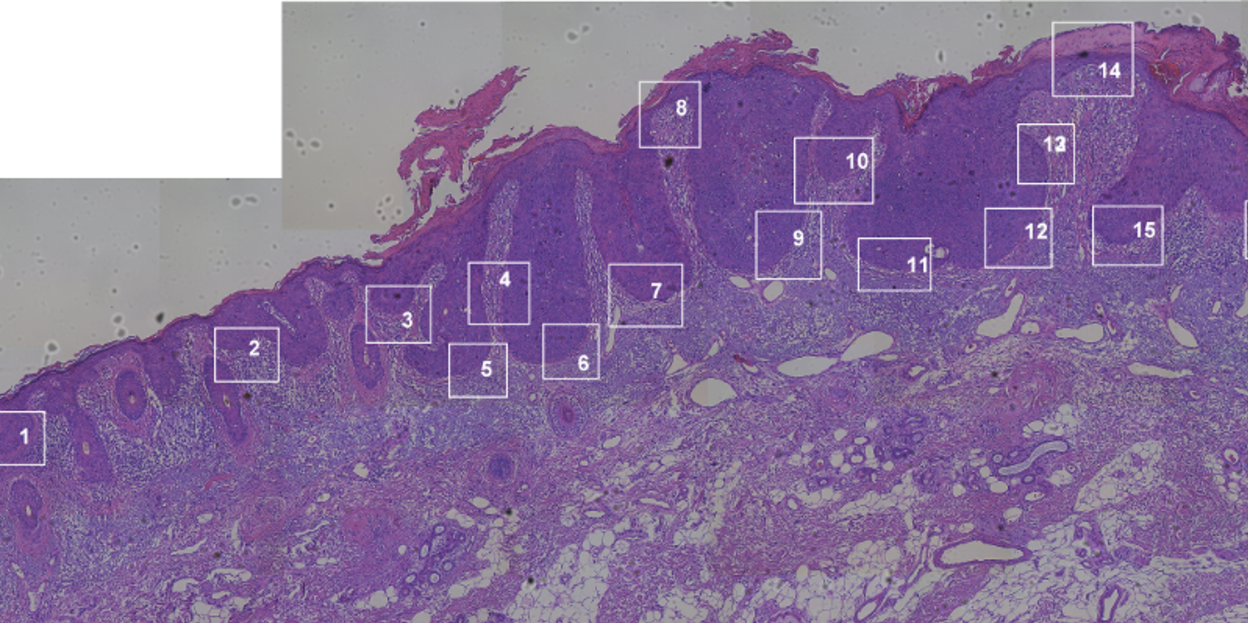
\includegraphics[width = 4.5 in]{cropped_zone_map_148185_11.pdf}} \\
\caption{Sample brightfield images, all showing (region 11 of) slide 148185. Image (a) is a manually aligned region, matching the MPM images in Figure \ref{fig:example_imageset_mpm} below. Image (b) is a high-resolution mini-mosaic of images captured around this region. Image (c) shows part of a full mosaic of all the images of this slide. Image (d) shows the same mosaic image, with regions of interest marked.}
\label{fig:example_imageset_bf}
\end{figure}

%Although the regions where MPM imaging was undertaken had been marked on the brightfield image mosaics, these annotations proved to be too approximate to be used as the ground truth against which to evaluate image registration methods in this study. 
The above image collection and pre-processing steps resulted in up to 10 separate images for each region of interest, even after combining the different polarization angles. To summarize these, for each region of interest we have the following images:
\begin{enumerate}
\item Brightfield image, a small sub-region from the stained slice, which has been resized, cropped, and rotated to align with an imaged MPM region (for 100 out of 400 regions)
\label{data:manual_bf}
\item High-resolution brightfield mini-mosaic centred on the region (stained)
\item Low-resolution brightfield mosaic of the whole histological block (stained)
\item Low-resolution brightfield mosaic of the whole histological block, with approximate location of region marked (stained)
\item SHG image, average of three polarization angles, of the unstained slice
\label{data:shg}
\item TPEF-NADH image, average of three polarization angles (unstained)
\item TPEF-FAD image, average of three polarization angles (unstained)
\item TPEF image, average of TPEF-NADH and TPEF-FAD images (unstained)
\label{data:tpef}
\item Processed MPM image, a combination of SHG image as blue channel and TPEF image as red channel, with gamma and constrast adjustments (unstained)
\item Greyscale MPM image, a conversion of the processed MPM image to greyscale (unstained)
\label{data:reprocessed_mpm}
\end{enumerate}
An example set of these 10 images is shown in Figures \ref{fig:example_imageset_bf} (brightfield images 1-4) and \ref{fig:example_imageset_mpm} (MPM images 5-10).

\begin{figure}
\centering
\subfloat[]{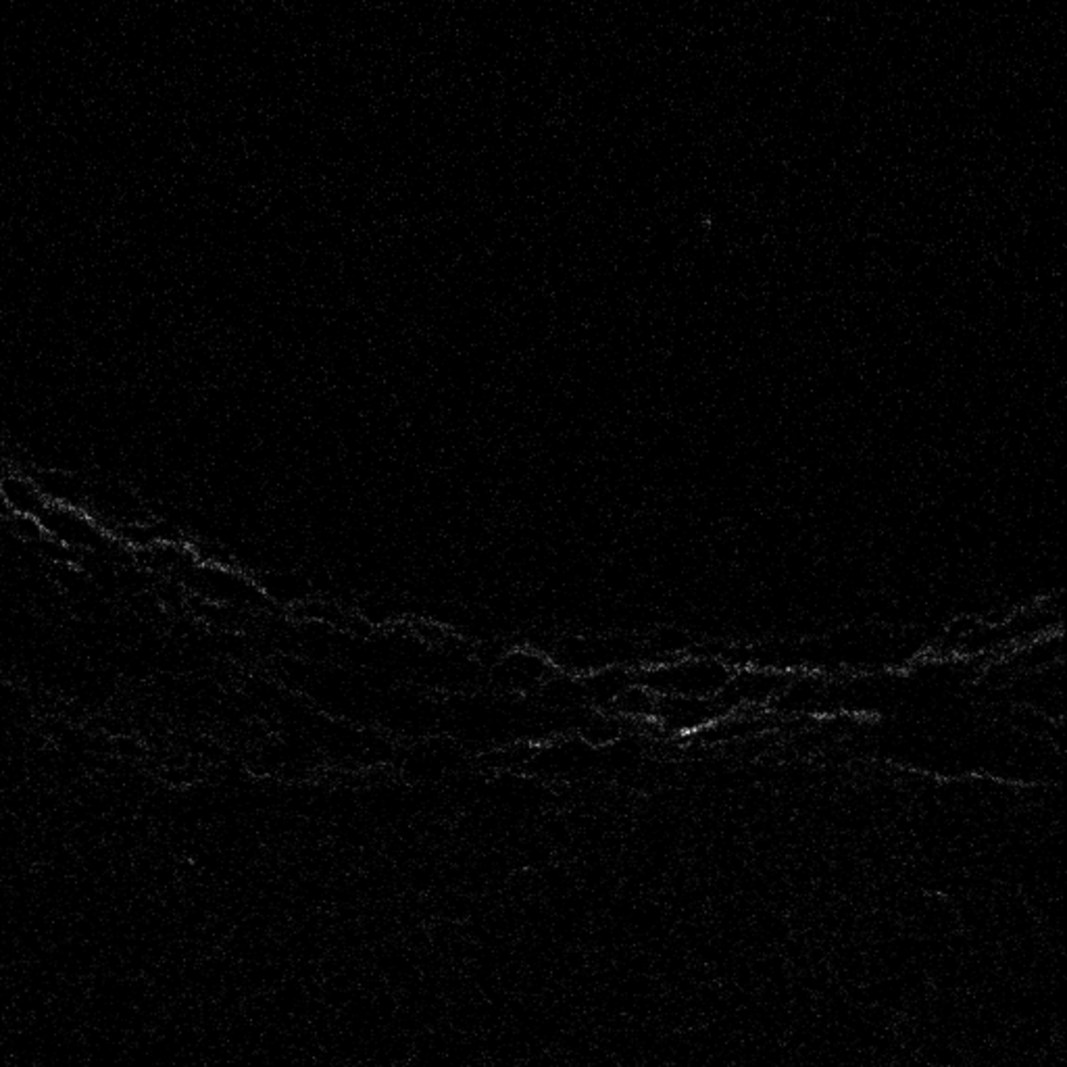
\includegraphics[width = 2 in]{SHG_148185_11_norm.pdf}} \
\subfloat[]{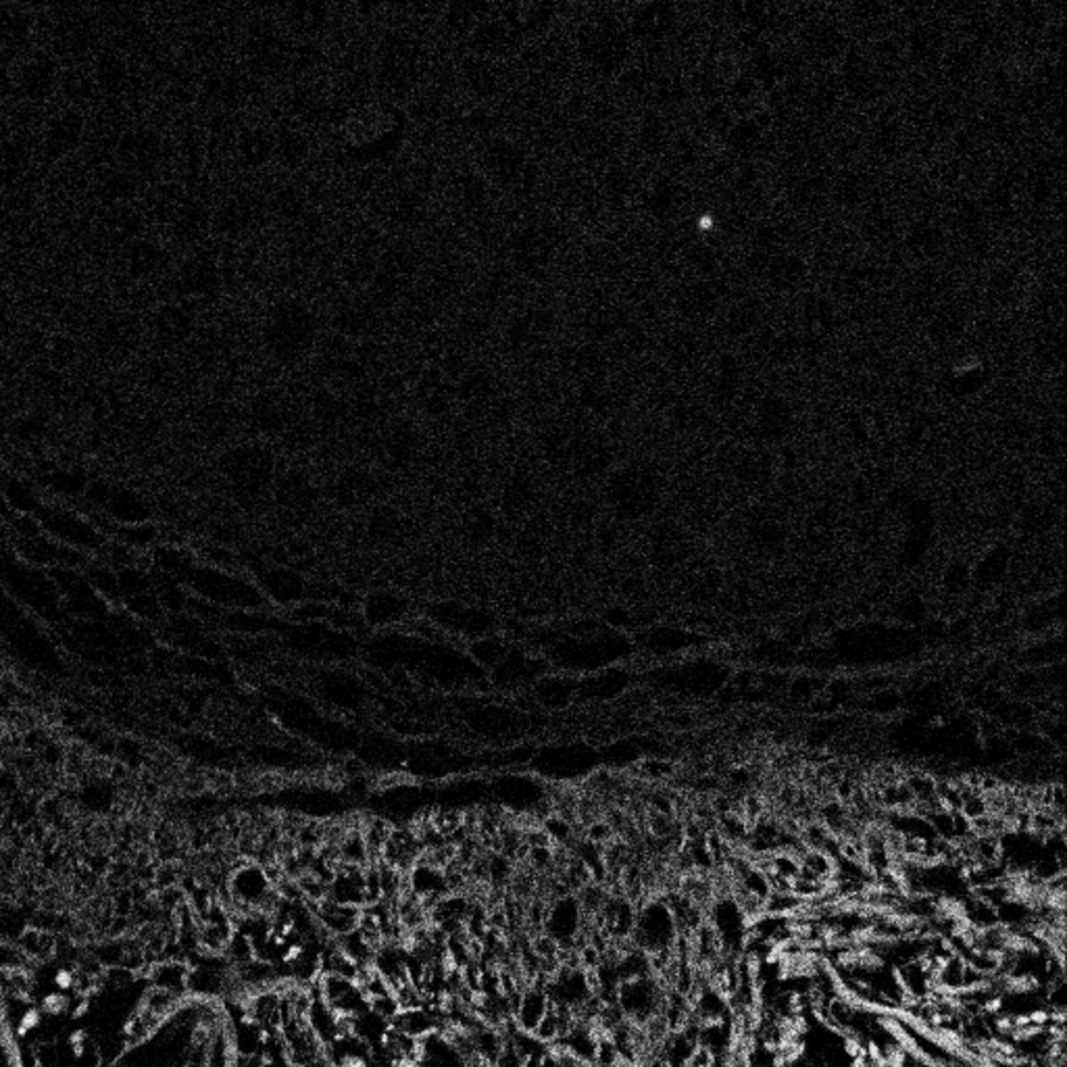
\includegraphics[width = 2 in]{TPEF1_148185_11_norm.pdf}} \\
\subfloat[]{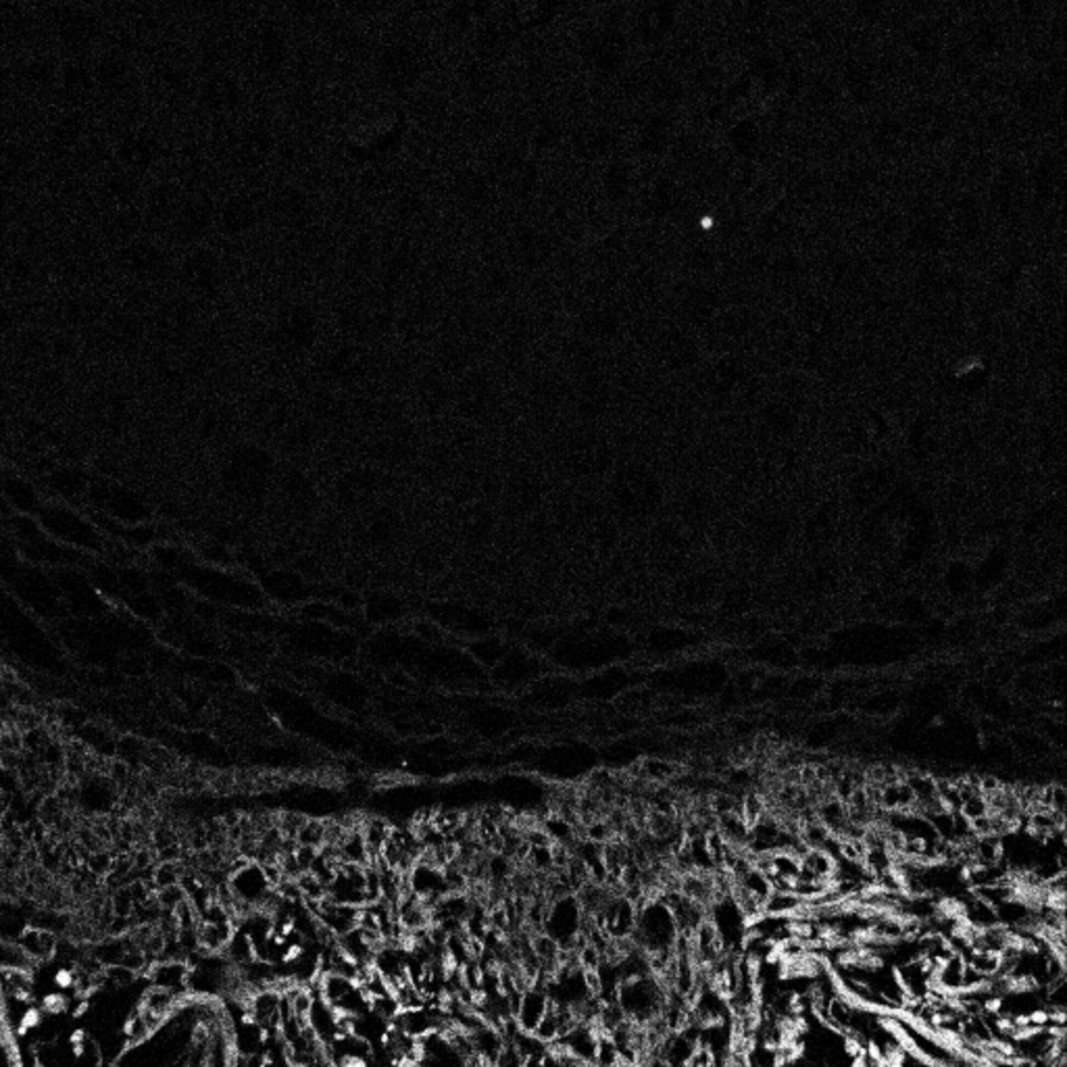
\includegraphics[width = 2 in]{TPEF2_148185_11_norm.pdf}} \
\subfloat[]{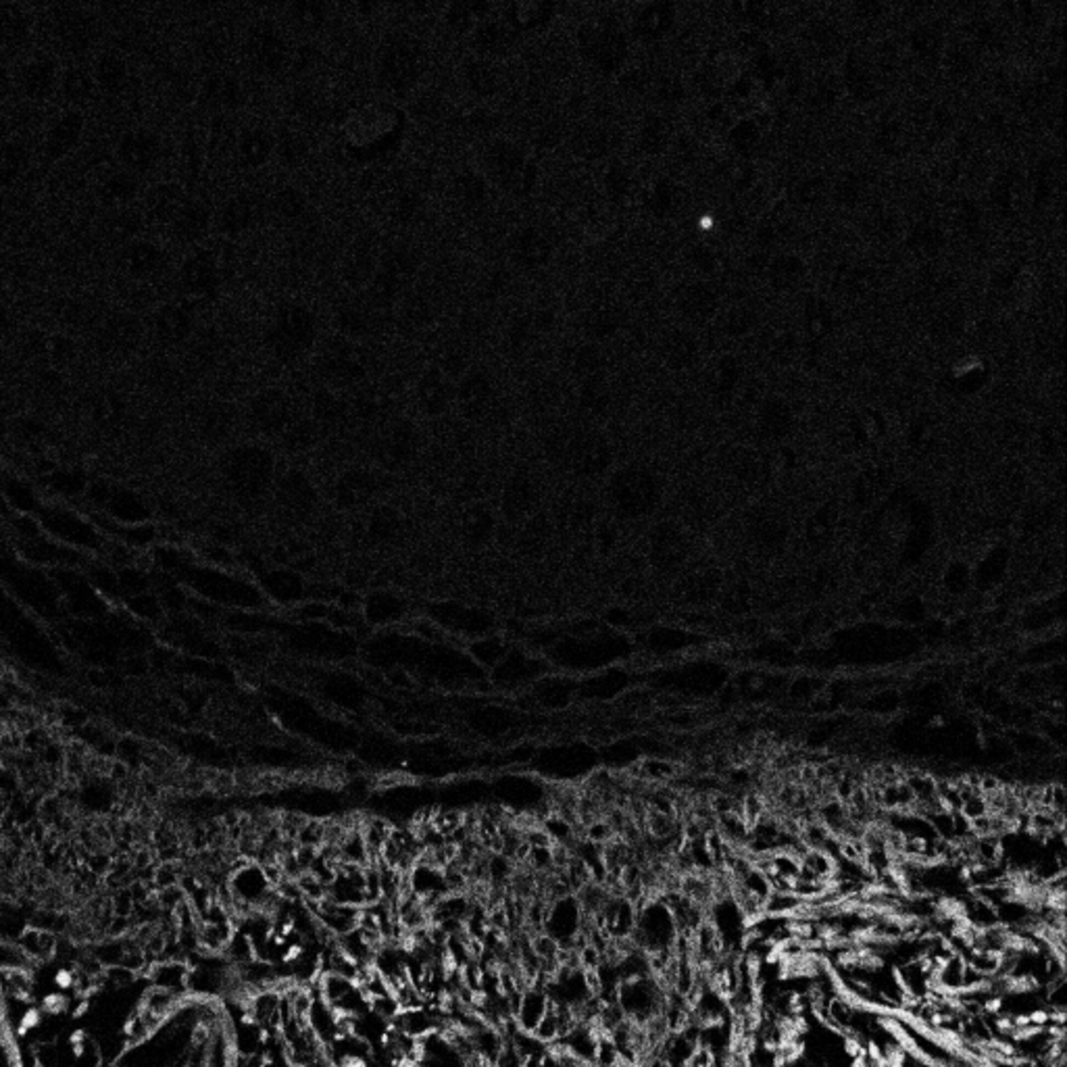
\includegraphics[width = 2 in]{148185_11_tpef_mean_norm.pdf}} \\
\subfloat[]{\includegraphics[width = 2 in]{processed_MPM_148185_11.pdf}} \
\subfloat[]{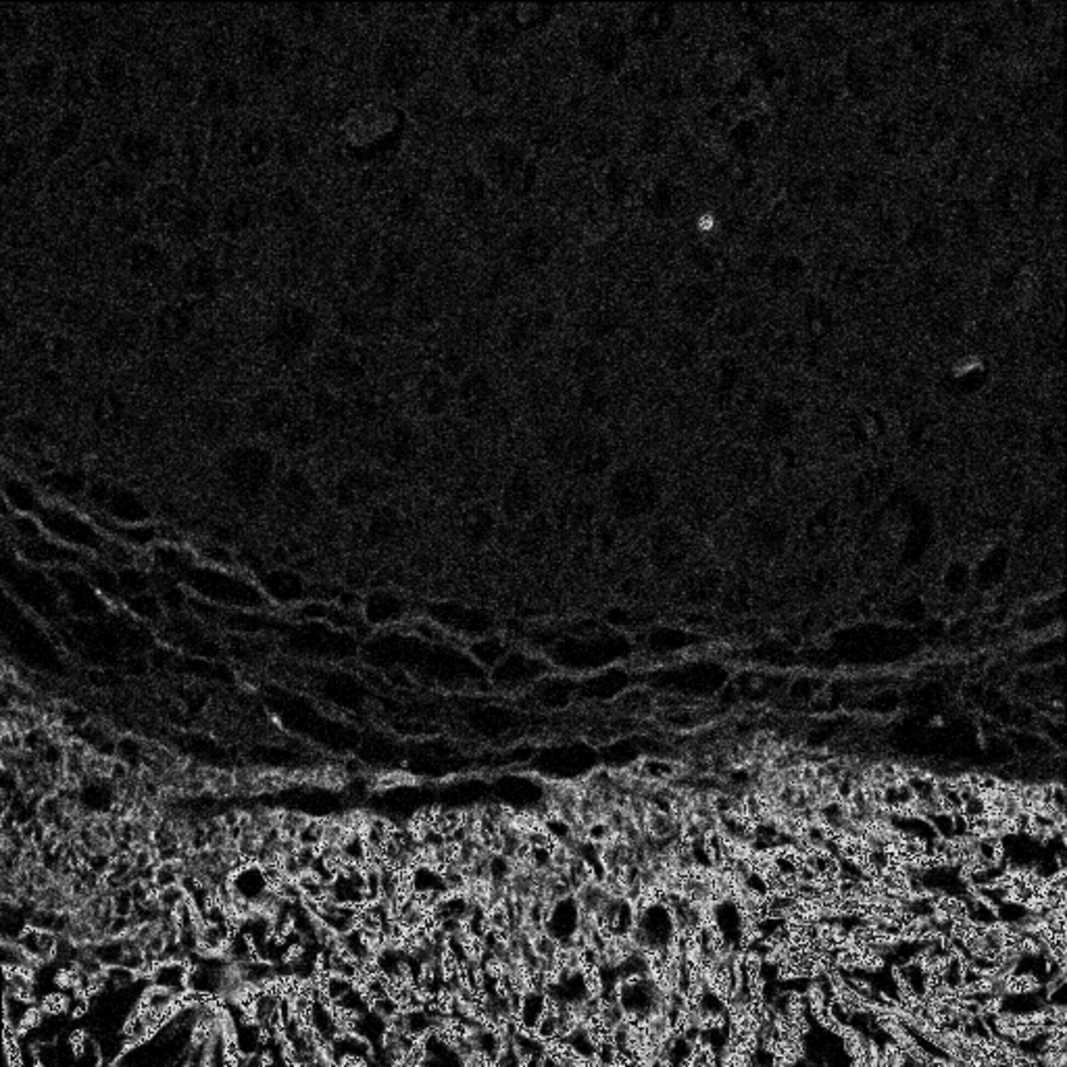
\includegraphics[width = 2 in]{reprocessed_MPM_gs_148185_11_norm.pdf}} \\
\caption{Sample MPM images, all showing region 11 of slide 148185. Image (a) is a Second Harmonic Generation (SHG) image, averaged over three polarization angles and normalized to improve contrast. Image (b) is TPEF-NADH, averaged over three angles and normalized. Image (c) is TPEF-FAD, also averaged and normalized. Image (d) shows the result of averaging images (b) and (c).
Image (e) is a contrast-enhanced combination of the first three, with SHG (a) as the blue channel and the average of the two TPEF images (d) as the red channel. Image (f) is a greyscale version of the combined MPM image, which has been normalized to improve the contrast.}
\label{fig:example_imageset_mpm}
\end{figure}
In this study, structural representation models are used to align images \ref{data:shg} with \ref{data:tpef} (Section \ref{sec:eval_shg_tpef}), and images \ref{data:manual_bf} with \ref{data:reprocessed_mpm} (Section \ref{sec:eval_bf_mpm}).

%TODO: decide what is to be done for bf/mpm and match here and below.

\chapter{Evaluation}
\label{sec:evaluation}
The main contribution of this study is to evaluate the relative performance of the models described above in Section \ref{sec:models}, in aligning multi-modal biomedical images. Each model was evaluated on the data described in Section \ref{sec:data} in a series of experiments which are described in this chapter. As a baseline for comparison, the Mutual Information between the images was also included.

The first task evaluated is to recover a known (random) transform $T^*$ applied to a SHG image, by finding the transform $\hat{T}$ which, when applied to the matching TPEF image, maximises some similarity measure between the TPEF image and the transformed SHG image, or between the structural representations of the same.

The second task similarly takes pairs of pre-aligned images, but this time the brightfield and the combined MPM images. As before a random transform is applied and then experiments are undertaken to recover the original transform. This is a step towards addressing the real challenge faced by our collaborators: to automatically find the location of an MPM image within a larger brightfield image. However, as will be seen below, the poor performance of the models under the controlled conditions evaluated on task 2 indicates that these methods are unlikely to be useful in pinpointing an MPM region at a completely unknown location within a brightfield image.

\section{Framework for evaluation of models}
Both models, along with Mutual Information, were implemented within a Python framework\footnote{https://github.com/MIDA-group/py\_alpha\_amd\_release}
developed for the $\alpha$-AMD registration model of \cite{ofverstedt2019fast}. This facilitates the comparison of results since all common functionality such as image pre-processing, application of transforms, and output formats is shared. The framework allows additional models and optimization methods to be added independently and applied in any combination, and incorporates various options such as parameter scaling, multiple start points, and masking.
%\citep{py_alpha_amd} 
\section{Task 1: Alignment of SHG and TPEF images}
\label{sec:eval_shg_tpef}

\begin{table}
\centering
\begin{tabular}{|p{1.2in}|p{1.05in}|p{0.6in}|p{0.9in}|p{0.9in}|}
\hline
\textbf{Registration Method} & \textbf{Pre-processing} & \textbf{Median error $E$ (px)} & \textbf{Successful registrations (\%)} & \textbf{Computation time} \\
\hline
\hline
1. NMI grid search & None & 2.26 & 100 & 26 mins \\
\hline
2. NMI gradient descent (multi-start) & Smoothing & 3.32  & 56 & 10 mins \\
\hline
\textbf{3. NMI gradient descent from result of 1} & \textbf{Smoothing} & \textbf{2.04}  & \textbf{100} & \textbf{27 mins} \\ 
\hline
4. PSR with NMI grid search & None & 4.08 & 64 & 30 mins \\
\hline
5. dLDP 48-bit grid search & Smoothing and Histogram Equalization & 2.61 & 96 & 51 mins \\
\hline
6. dLDP 48-bit gradient descent from result of 5 & Smoothing and Histogram Equalization & 2.08  & 96 & 52 mins \\
\hline
\end{tabular}
\caption{Results for Task 1: Alignment of SHG and TPEF images. 25 pairs of pre-aligned images, with a known transform applied to one image in each pair, were aligned using each method. The median error $E$ is given for each method, along with the proportion of registrations for which $E<5$ (these are considered successful registrations). Computation times given are approximate times per image pair on standard consumer hardware, and have not been thoroughly optimized.}
\label{tab:task1results}
\end{table}


As described in Section \ref{sec:data}, for each region of interest one SHG and two TPEF images were constructed by taking the average of the images obtained from three different incident polarization angles. The two TPEF images were combined into a single image by averaging the intensities at each pixel. The resulting pair of images (SHG and TPEF) are already aligned, as they are captured using the same equipment on the same tissue slice at the same time.

In this section, a series of experiments is used to evaluate the ability of different methods to recover a known (synthetic) transform.

All transforms used in this section are restricted to isotropic scale, rotation, and translation changes. No shearing or non-rigid deformations are applied. A transform $T$ can therefore be described by a vector of four parameters, $T=[T_s, T_r, T_x, T_y]$, where $T_s$ is the scaling transform, measured as a proportion of the image size, $T_r$ is the rotation transform, measured in degrees, $T_x$ is the translation in the horizontal direction, measured in pixels, and $T_y$ is the translation in the vertical direction, also measured in pixels.

For each pair of matching SHG and TPEF images, a random transform $T^*$ was constructed by choosing the four parameters uniformly within the following ranges: $0.95\leq T^*_s\leq 1.05$; $-5\leq T^*_r\leq 5$; $-10\leq \{T^*_x, T^*_y\}\leq 10$. This transform was applied to the SHG image, using nearest neighbour interpolation, giving a reference image $I_R = T^*(I_{SHG})$. The experiments below aim to estimate the transform $\hat{T}$ which, when applied to the TPEF (floating) image $I_F$, results in the best alignment.

The quality of the resulting transform is evaluated by calculating the Euclidean distance between the position of each corner of the transformed floating image ($\hat{T}(I_F)$) and the position of the corresponding corner of the reference image ($I_R$), and taking the mean:
\begin{equation}
E = \frac{1}{4} \sum_{i=0}^{3} | \hat{T}(c_i) - T^*(c_i) |,
\label{eq:E}
\end{equation}
where $c_i$ denotes the position of image corner $i$, for $i \in \{0,...3\}$
%Further, when $E<\epsilon$ pixels, the registration is considered successful.

Experiments with the two structural representation models, and with Mutual Information, are described separately in Sections \ref{sec:mi_results} to \ref{sec:model2_results} below. The same regions and transforms were used for each model to ensure comparability of results. The best results from each method are summarized in Table \ref{tab:task1results}, which compares the median value of $E$ obtained when registering 25 test image pairs, along with the proportion of registrations considered successful (see Section \ref{sec:success} below), and the computation time required for each pair of images. All timings are approximate, and were recorded on a four core (two physical core) Intel i7 processor running Ubuntu, with 16GB RAM. Although not one of the best performing methods in terms of accuracy, the results for NMI gradient descent (from multiple starting points) is included in this table because of its superior computational performance.

\subsection{Success measure for registrations}
\label{sec:success}
\begin{figure}
\centering
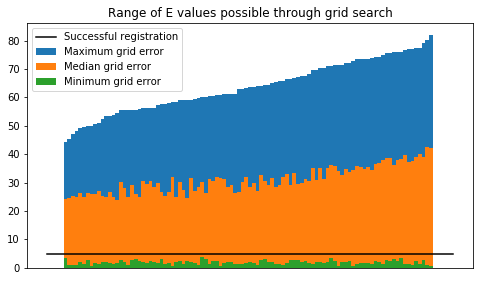
\includegraphics[width=5in]{grid_Es_2.png}
\caption{Selection of threshold for successful registration. Plot shows minimum, median, and maximum values of $E$ that can be obtained with the specified grid search parameters, for 100 random transforms (sorted by maximum grid search error). Based on these results a threshold of 5 pixels was chosen, so that registrations with $E<5$ (black line) are considered successful in this study. The average proportion of grid points that lie below this threshold is 0.26\%.}
\label{fig:grid_errors}
\end{figure}

To facilitate comparison of methods, a binary measure of whether a registration is successful is helpful. The error measure $E$, defined above in Equation \ref{eq:E}, gives a numerical accuracy measure which can be thresholded to indicate whether a registration can be considered successful or not. In several experiments in this chapter, transforms on a parameter grid are used to evaluate the method, and this parameter grid is tightly specified within the same parameter ranges as the random transforms that constitute the ground truth.

The threshold must therefore be carefully chosen to ensure that randomly selected grid points are not expected to lie within the success range, but that the closest grid point should be considered a successful registration. To set the threshold, a selection of 100 random transforms are chosen, and for each one the value of $E$ at each grid point is calculated.

Values of $E$ under these conditions can be as much as 80 pixels, depending on how extreme the random transform chosen is. The minimum error depends on how close the random transform is to a grid point. This is illustrated in Figure \ref{fig:grid_errors}. The minimum error (i.e. the value of $E$ at the closest grid point) for this selection of random transforms ranges between 0.42 and 3.64 pixels. A value of $E=5$ pixels was therefore chosen for the success threshold. The vast majority (99.74\%) of grid points correspond to an error greater than this threshold, so the likelihood of false positives (successful registrations reported by chance, when model outputs are incorrect) is low.

The same threshold value is applied to gradient descent methods, in which the maximum error values are unbounded.


\subsection{Alignment with Mutual Information}
\label{sec:mi_results}
Although Mutual Information (MI) has been shown to be an excellent similarity measure for multi-modal images,
a major drawback is that it is often difficult to find the maximum MI position, since the MI surface tends to have many local maxima and an extremely narrow peak at the true alignment, particularly in the presence of noise \citep{maes1997multimodality}. 

The following experiments were used to find the transform maximising the MI between $I_R$ and $T(I_F)$. Since transforming the floating image can reduce the amount of overlap between the images, which tends to increase the MI, in all cases the Normalized Mutual Information was used. In additions, where the overlapping area dropped below 40\% of the pixels for a given transform, the NMI was set to zero, to avoid bias towards extreme transforms.

Before calculating the NMI, image intensities were quantized into 32 bins. This step reduces the effects of noise on the MI calculations. All interpolation was done using nearest neighbour interpolation. Other interpolation schemes tend to lead to smoothing of the images, which can affect the distance measures being evaluated, particularly when the images have not been smoothed to begin with. By first choosing whether to smooth the image, and then using nearest neighbour interpolation, these effects can be better controlled.

\begin{table}
\centering

\begin{tabular}{|p{1.55in}|p{0.75in}|p{1.5in}|p{1.2in}|}
\hline
\textbf{MI Maximization Method} & \textbf{Pre-processing} & \textbf{Median error $E$ (px)} & \textbf{Successful registrations (\%)} \\

\hline
\hline
1. Grid Search & None & 2.26 & 100  \\
\hline
2. Grid Search & Smoothing & 2.88 & 80  \\
\hline
3. Gradient Descent from identity transform & None & 20.96  & 4 \\ 
\hline
4. Gradient Descent from identity transform & Smoothing & 8.34  & 24 \\ 
\hline
5. Gradient Descent from 20 random points & None & 89.8  & 40 \\ 
\hline
6. Gradient Descent from 20 random points & Smoothing & 3.32  & 56 \\
\hline
\textbf{7. Gradient Descent from result of 1} & \textbf{Smoothing} & \textbf{2.04}  & \textbf{100} \\ 
\hline
\end{tabular}
\caption{Results of using Mutual Information to align SHG and TPEF images. The transform $\hat{T}$ that maximised the mutual information for each image pair ($I_R$, $\hat{T}(I_F)$) was sought. The average distance $E$ between the location of the image corners when transformed using the ground truth transform $T^*$ and when transformed using $\hat{T}$ was calculated for each image pair. The same 25 regions, with the same set of random transforms applied, were used for each method, and the median of $E$ is shown along with the proportion of estimates for which $E<5$ pixels. Note that in experiment 7, the optimal grid point from experiment 1 (unsmoothed images) was used as the starting point for a gradient descent using smoothed images.}
\label{tab:MIresults}
\end{table}


\subsubsection{Mutual Information grid search}
The normalized mutual information was evaluated at a range of transforms $T = [T_s, T_r, T_x, T_y]$ using the parameter grid:
\begin{itemize}
    \item $95\% \leq T_s \leq 105\%$, in steps of 1\%
    \item $-5 \leq T_r \leq 5$, in steps of 1 degree
    \item $-10 \leq \{T_x, T_y\} \leq 10$, in steps of 2 pixels
\end{itemize}
The range of this grid matches the range of random transforms that were applied to the SHG image to create $I_R$. In real applications of multi-modal image registration, it is rare that the true range of transformation parameters could be estimated within such a small margin, although the correct scale could sometimes be accurately estimated from knowledge of the magnifications used when capturing the images. Using a bigger parameter grid would approximate more closely the results that might be achieved in real-world applications, but calculation of mutual information is too  time-consuming for a more extensive evaluation to be undertaken in this study.


The grid search was repeated after applying smoothing (Gaussian smoothing with $\sigma = 3.0$) and intensity normalization, such that for an image with intensity $I(x)$ at pixel $x$, 
\[
I'(x) = \frac{I(x)-\text{min}(I)}{\text{max}(I)-\text{min}(I)}.
\]

The smoothing and normalization were applied to both the reference and the floating image. Results are shown in Table \ref{tab:MIresults}.

\subsubsection{Mutual Information gradient descent}
Since a grid search in four dimensions is extremely time consuming and, unless a very fine grid, or a suitable refinement scheme is used (further increasing the computation time), also rather inaccurate, a gradient descent method for finding the MI maximum is also evaluated here. The Broyden–Fletcher–Goldfarb–Shanno (BFGS) algorithm was used, after rescaling the transform parameters such that the order of magnitude of the translation, rotation, and scaling would be equivalent. In this method, the gradient is estimated numerically by making a small change to each parameter in turn. A step is then taken in the direction of steepest descent, and the gradient is recalculated. Step sizes are calculated using a line search algorithm. A library implementation\footnote{https://www.scipy.org/} of the BFGS algorithm was used.

Results are shown for three different strategies: 
\begin{enumerate}
    \item Initialize the search at the identity transform
    \item Initialize the search at 20 additional random starting points, selected uniformly from within the parameter range described above, and choose the one which results in the highest NMI
    \item Initialize the search at the best transform found in the grid search above
\end{enumerate}
As above, each experiment was repeated with and without first smoothing the images using a Gaussian filter. Results are given in Table \ref{tab:MIresults}. For the gradient descent methods, smoothing the images led to a big improvement in the number of successful registrations and the median error $E$.

Experiment (2), as with the above grid search, assumes that the range of possible transforms is known to within a reasonably close approximation. Experiment (3) is even more computationally expensive than the grid search, although the additional gradient descent step only adds a relatively small computational cost compared to the grid search, and results show an improvement over the grid search (see Table \ref{tab:MIresults}).

\subsubsection{Mutual Information evaluation}
As shown in Table \ref{tab:MIresults}, the best results were achieved when starting a gradient descent search method from the maximum found on a grid of transforms (experiment 7), but good results were also obtained by using a gradient descent method with a multi-start approach (experiment 6). The time taken for the latter was less than half of that taken for the combination of a grid search plus a gradient descent.

Smoothing the images reduced the proportion of successful registrations in the grid search experiment. In several cases, including most of the `failures', the value of the NMI metric was higher at the chosen gridpoint than at the ground truth. This may perhaps be attributed to individual noise pixels from the original image being `smeared' across several pixels in the smoothed images, so that instead of affecting the metric at only a single pixel, the effect is amplified. One example is shown in Figure \ref{fig:MI_surfaces}, which gives the NMI surface for a grid small perturbations from the ground truth alignment, for a (particularly challenging) pair of aligned SHG and TPEF images. Although only two of the four grid dimensions can be illustrated here, multiple local optima can be seen in the first row (which shows NMI values over a coarse grid of parameter values), and they appear stronger in the smoothed image. Even within a very short range of the ground truth position, the use of smoothed images does not necessarily lead to a smoother surface (fine grid, second row).

\begin{figure}
\centering
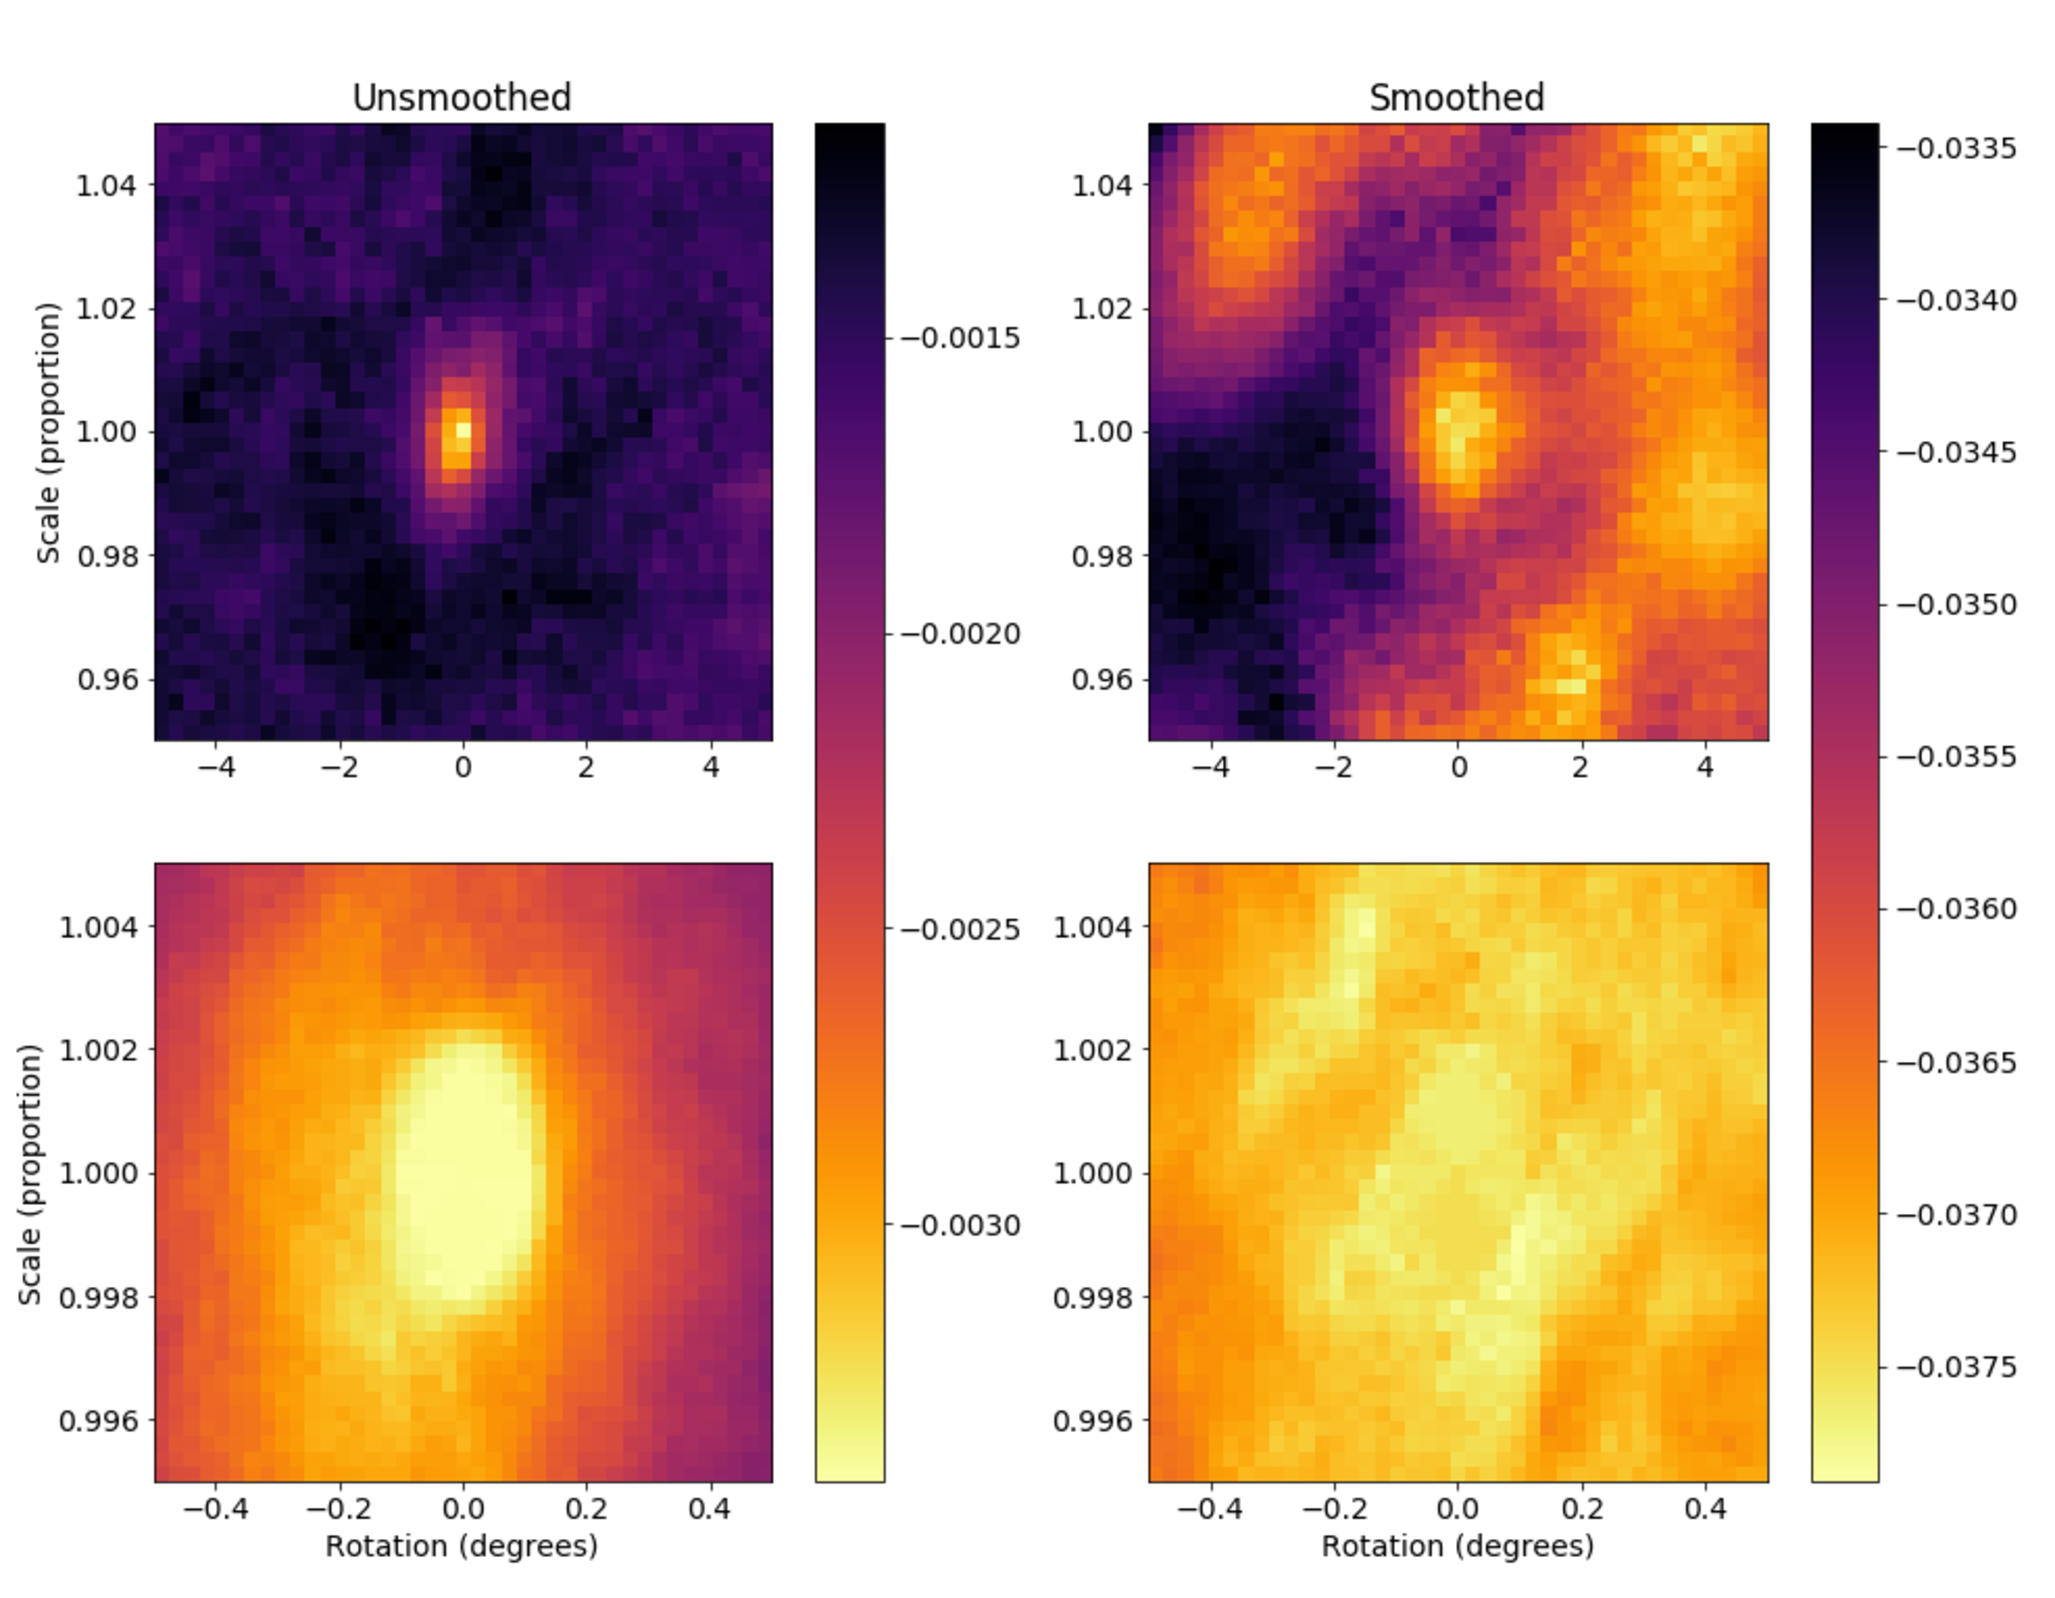
\includegraphics[width=5.5in]{bothgrids_bothblur_im20.pdf}
\caption{Mutual Information surfaces for smoothed and unsmoothed versions of the same pair of aligned images. In the first row, a coarse grid is shown, covering the full parameter range used in this study (up to 5 degrees rotation and up to 5\% scale difference). The translation parameters were fixed at 0 pixels for this illustration. The local optima visible around the edges of the unsmoothed surface are much more pronounced in the smoothed version, and the peak does not lie in the correct position. The maximum NMI for the unsmoothed version is found at the ground truth position $(T_r, T_s) = (0, 1)$ with NMI=0.00343 and $E=0$. For the smoothed version, the maximum lies at (2, 0.96) which has NMI=0.0377 and $E=23.8$. This is higher than the NMI at the ground truth, which for smoothed images is 0.0375. In the second row, a fine grid of parameter values is used, covering rotation of up to 0.5 degrees and scale differences of up to 0.5\%. The optimum grid point for the unsmoothed image is (0.075, 0.999), giving NMI=0.00344 (marginally higher than at the ground truth) and $E=0.72$. For the smoothed image the peak at (0.1, 0.99875) is less defined and gives NMI=0.0379 (also higher than at the ground truth) and $E=0.94$. Within such a fine grid around the origin it is relatively easy to choose a transform with $E<5$. }
\label{fig:MI_surfaces}
\end{figure}

For gradient descent, smoothing the images helped the algorithm by increasing the size of the attraction region, where the NMI gradient leads in the direction of the optimum, but the success rate remained low. In some cases (both with smoothed and unsmoothed images), the gradient descent method found an optimum transform with a higher NMI score than that at the ground truth (see example in Figure \ref{fig:MI_surfaces}). Further work to tune the gradient descent parameters, and to penalize extreme transforms, would be likely to improve these results somewhat. However, given that the NMI maximum for smoothed images does not necessarily coincide with the position of the ground truth, and given the difficulty of following gradients on unsmoothed images, this method is unlikely to ever achieve highly accurate registration results on this dataset.

\subsection{Alignment with Model 1: PCANet-based Structural Representations of multi-modal images}
\label{sec:evalPSR}
%TODO check once all results are in
\begin{table}
\centering
\begin{tabular}{|p{1.2in}|p{1.05in}|p{0.75in}|p{0.6in}|p{0.9in}|}
\hline
\textbf{PSR Alignment Method} & \textbf{Image pre-processing} & \textbf{PSR smoothing} & \textbf{Median error $E$ (px)} & \textbf{Successful registrations (\%)} \\
\hline
\hline
\textbf{1a. MI Grid Search} & \textbf{Smoothing} & \textbf{False} & \textbf{4.08} & \textbf{64} \\ %PartII_test1.2
\hline
1b. MI Grid Search & Smoothing & True & 11.14 & 16 \\ %PartII_test1.3
\hline
2a. MI Grid Search & Smoothing and Histogram Equalization & False & 5.44 & 48 \\ %PartV_test1.2
\hline
2b. MI Grid Search & Smoothing and Histogram Equalization & True & 17.49 & 32 \\ %PartV_test1.3
\hline
%Not much point in MI gradient descent if the max is not at the GT, skip non-smoothed tests
3. MI Gradient Descent from multiple start points & Smoothing & False & 42.06 & 20 \\ %PartII_test2b.2
\hline
4. MSE Grid Search & Smoothing & False & 10.75  & 32 \\ %PartII_test3.2
\hline
%5. MSE Grid Search & True & todo  & todo \\ %Haven't got results for the same regions but the ones I have done are terrible
%\hline
%5. MSE Gradient Descent & Smoothing & False & todo  & todo \\ 
%\hline
% 6. $\alpha$AMD Grid Search & False & todo  & todo \\ 
% \hline
% 7. $\alpha$AMD Gradient Descent & False & todo  & todo \\ 
% \hline
\end{tabular}
\caption{Results of using PCANet-based structural representations to align SHG and TPEF images. The PSR images are first created, using smoothed and (in some tests) histogram equalized versions of the SHG and TPEF images. The registration of these PSR images is then attempted, with and without smoothing. The average distance $E$ from the corners of the registered images to their ground truth positions is calculated. If $E<5$ pixels, the registration is considered successful. The best results with Mutual Information were obtained after training the model on smoothed (experiments 1a and 1b), but not histogram equalized (experiments 2a and 2b), versions of the original images, and with no smoothing applied to the resulting PSRs (experiment 1a). These settings were used for the remaining tests (experiments 3-4).}
\label{tab:PSRresults}
\end{table}

A structural representation of each SHG and TPEF image was created using the method of \cite{zhu2018pcanet} which is described above in Section \ref{sec:model1}.

Each image was first normalized and then smoothed using a Gaussian filter with $\sigma=3.0$, to reduce the amount of noise apparent in the structural representation. The difference is shown in Figure \ref{fig:tuningPSR}, where for two example hyperparameter settings ($c1=c2=0.01$ and $c1=c2=0.1$), the PSRs resulting from training with unsmoothed and unsmoothed versions of the TPEF images are shown. 

The model was then tuned by undertaking training with each combination of values of $c_1$ and $c_2$ in \{0.01, 0.05, 0.1, 0.2, 0.5\}, and inspecting the resulting structural representations for clarity and visibility of the common structures within an image.
Values of $c_1=c_2=0.2$ were chosen for SHG images whilst $c_1=c_2=0.1$ gave the clearest structural representations for TPEF images, as shown in Figure \ref{fig:tuningPSR}. The full set of example PSRs for networks trained with these values of $c1$ and $c2$, for both TPEF and SHG images, is shown in Appendix \ref{appendix:tuning}. For each modality, the network, consisting of two layers of eight $3 \times 3$ filters, was trained on a random subset of 100 images.

\begin{figure}
\centering
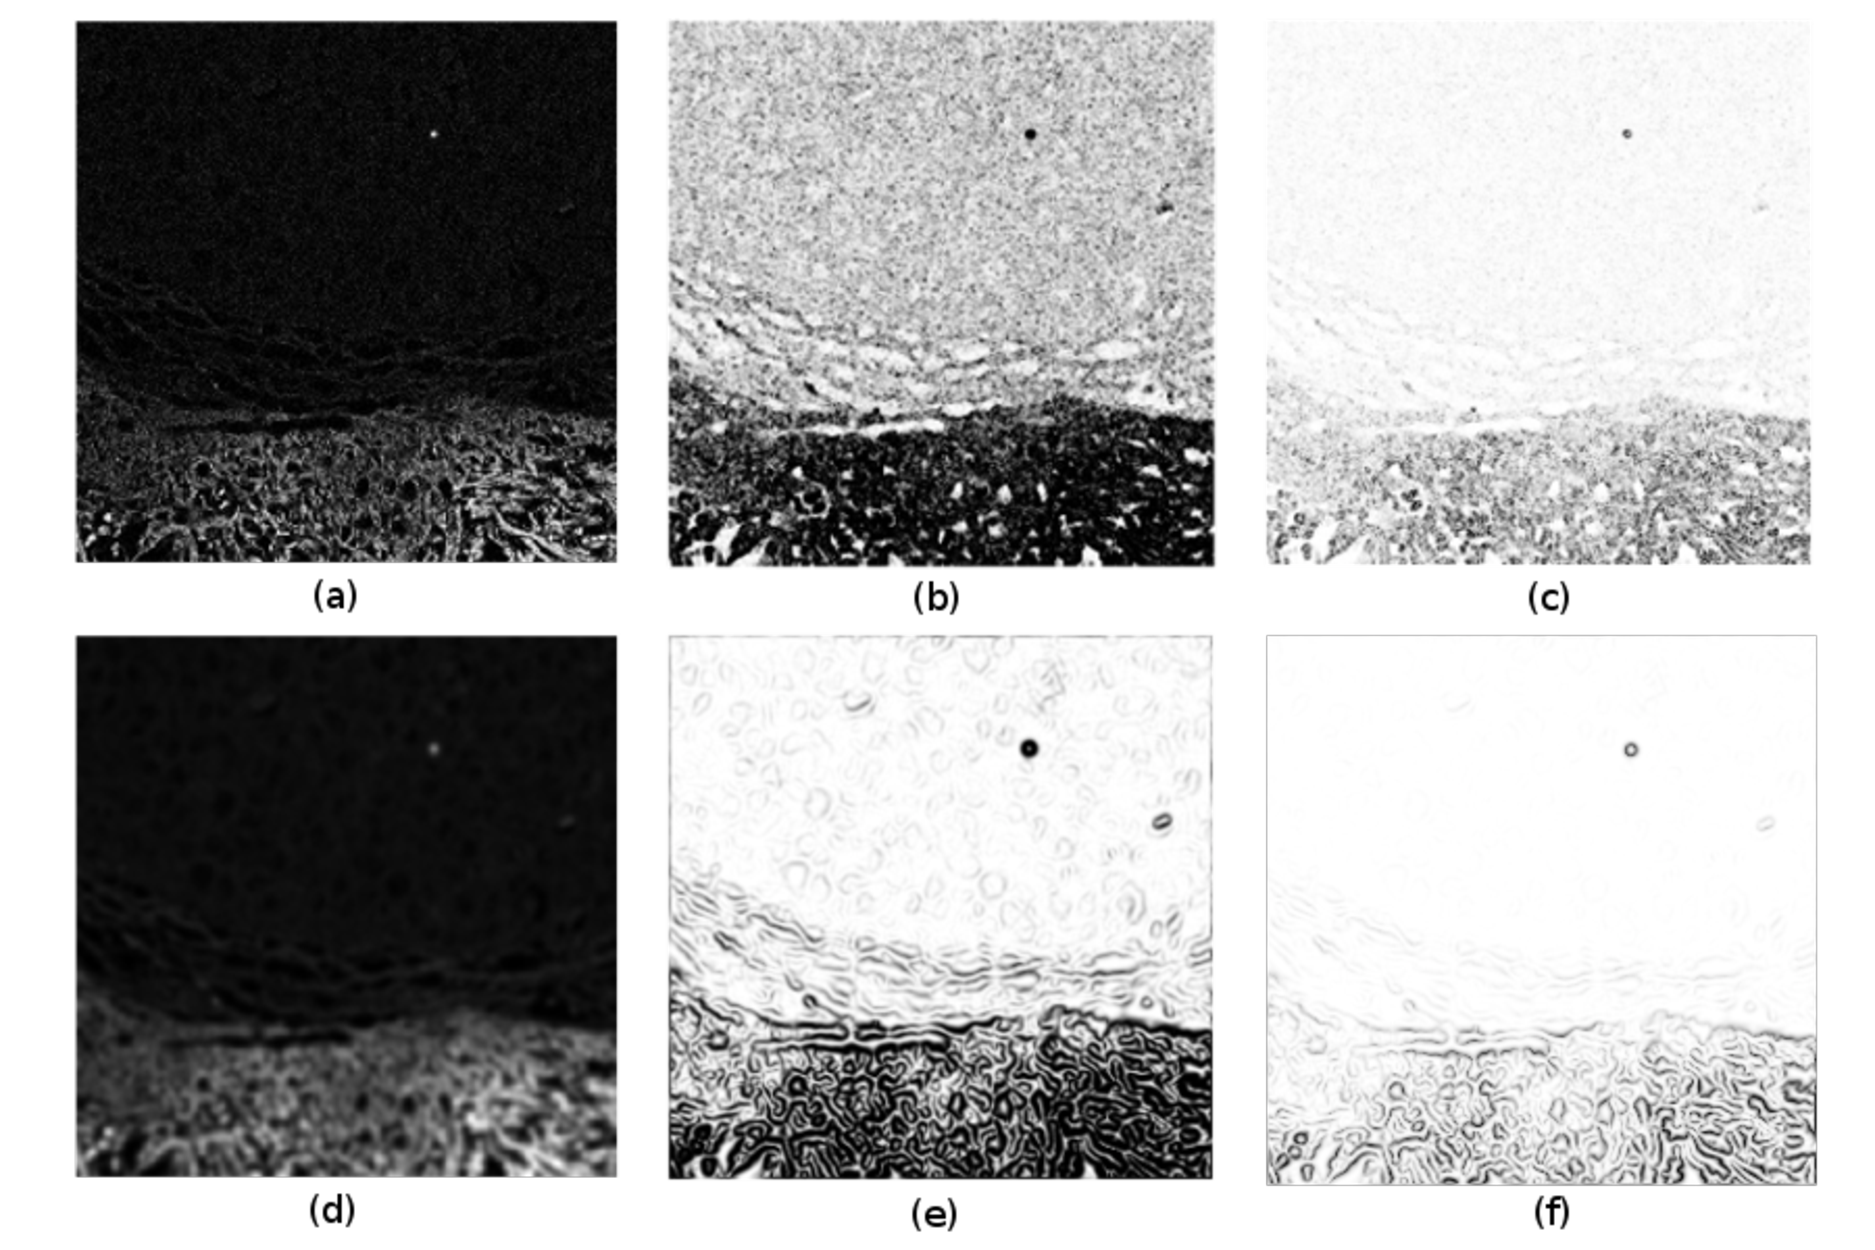
\includegraphics[width=5.75in]{tuning_tpef_148185_11.pdf}
\caption{PCANet-based structural representations of TPEF images. The top row shows (a) the original (normalized) TPEF image, (b) the structural representation of this image using PSR parameters $c_1=c_2=0.01$, (c) the structural representation of this image using parameters $c_1=c_2=0.1$. The structure is not well-defined due to the noisy, high-frequency image modality. The second row shows the same as the first row except based on a smoothed version of the original image (d), using a Gaussian filter with $\sigma=3$. Here the structural representations depict the image features more clearly. The first structural representation (e), with $c_1=c_2=0.01$, includes a lot of fine detail which is not expected to be useful in aligning the images. The second version (f) was chosen for this modality, with parameters $c_1=c_2=0.1$.}
\label{fig:tuningPSR}
\end{figure}

The trained networks were used to produce a structural representation of each image, which can then be aligned using standard mono-modal registration techniques. The techniques evaluated in this study were Normalized Mutual Information (NMI) and Mean Squared Error (MSE). %and Alpha-AMD ($\alpha$AMD) \citep{ofverstedt2019fast}. 

The above experiments were also repeated using histogram-equalized versions of the images. The networks were retuned (parameters chosen were $c_1=0.1$, $c_2=0.01$ for SHG, and $c_1=0.01$, $c_2=0.1$ for TPEF) and retrained to produce a second set of structural representations.

Results are shown in Table \ref{tab:PSRresults}. Grid search and gradient descent parameters were the same as described in Section \ref{sec:mi_results} above. Whilst the best results were obtained by aligning the PSRs with Mutual Information, the results are worse than those obtained by aligning the original images with Mutual Information. For smoothed PSRs, in most cases the highest Mutual Information position does not match the ground truth registration position, as shown for one example region in Figure \ref{fig:MIsurfacePSR}, so no gradient descent was attempted with smoothing. 

\begin{figure}
\centering
\subfloat[]{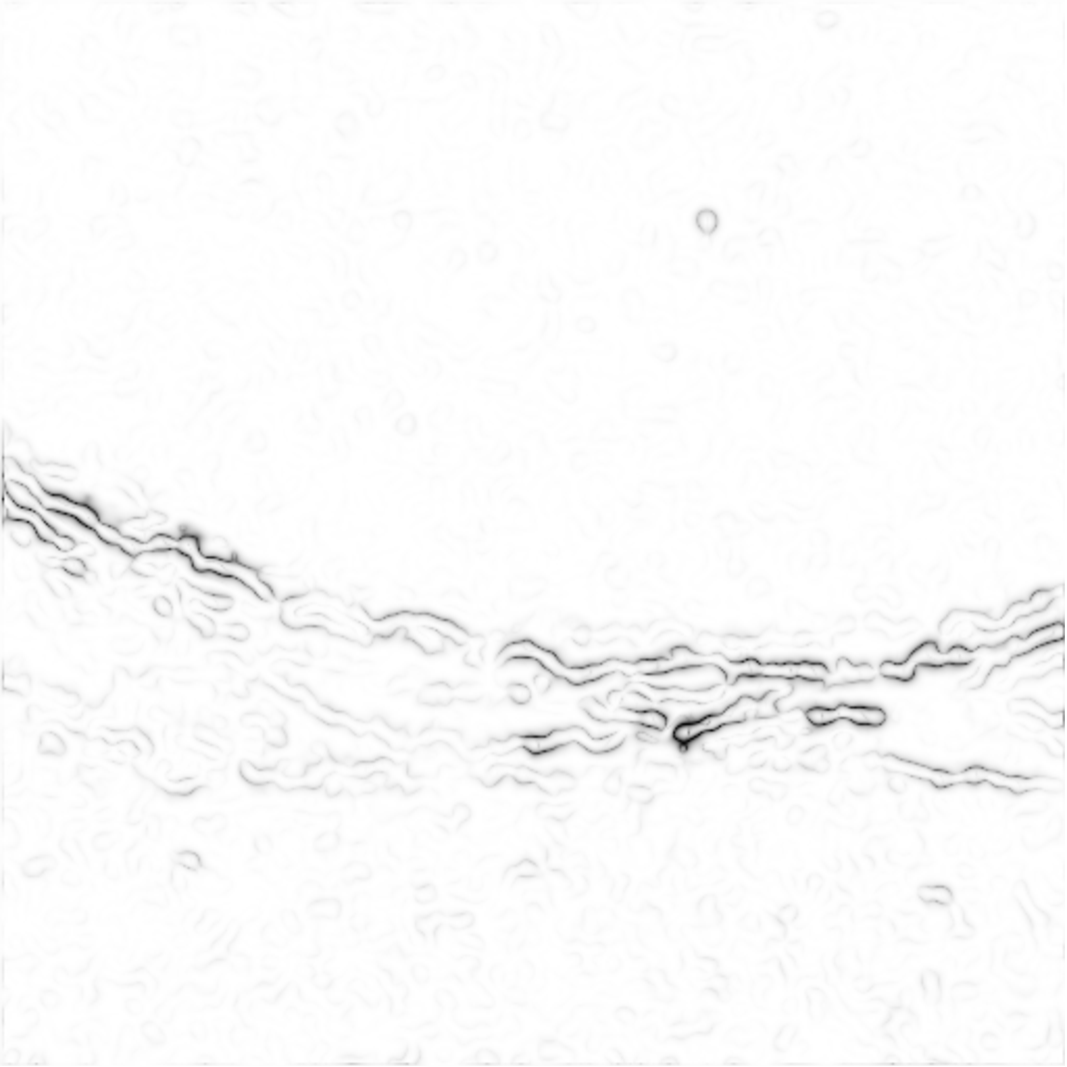
\includegraphics[width = 2.5 in]{psr_shg_148185_11.pdf}} \
\subfloat[]{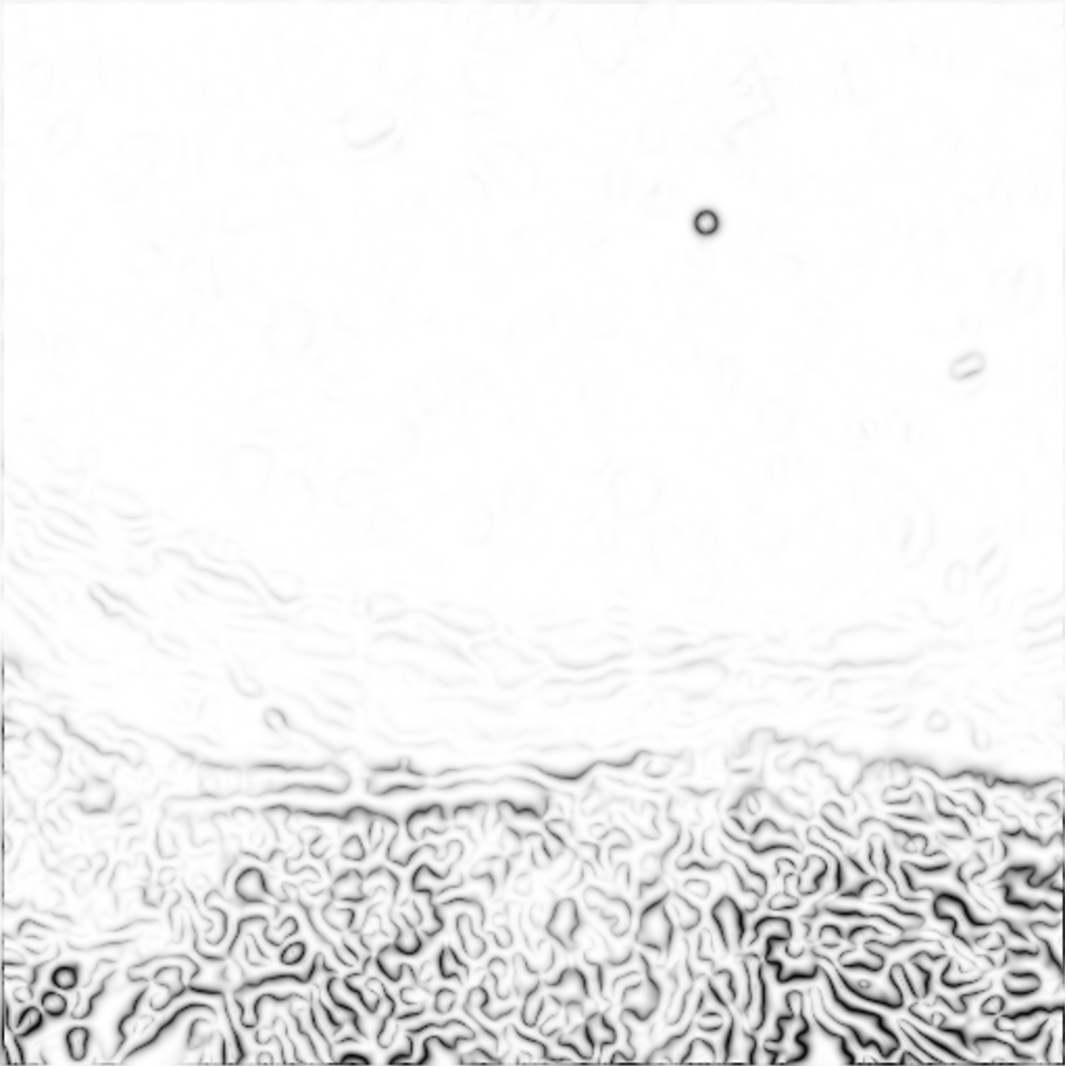
\includegraphics[width = 2.5 in]{psr_tpef_148185_11.pdf}} \
\subfloat[]{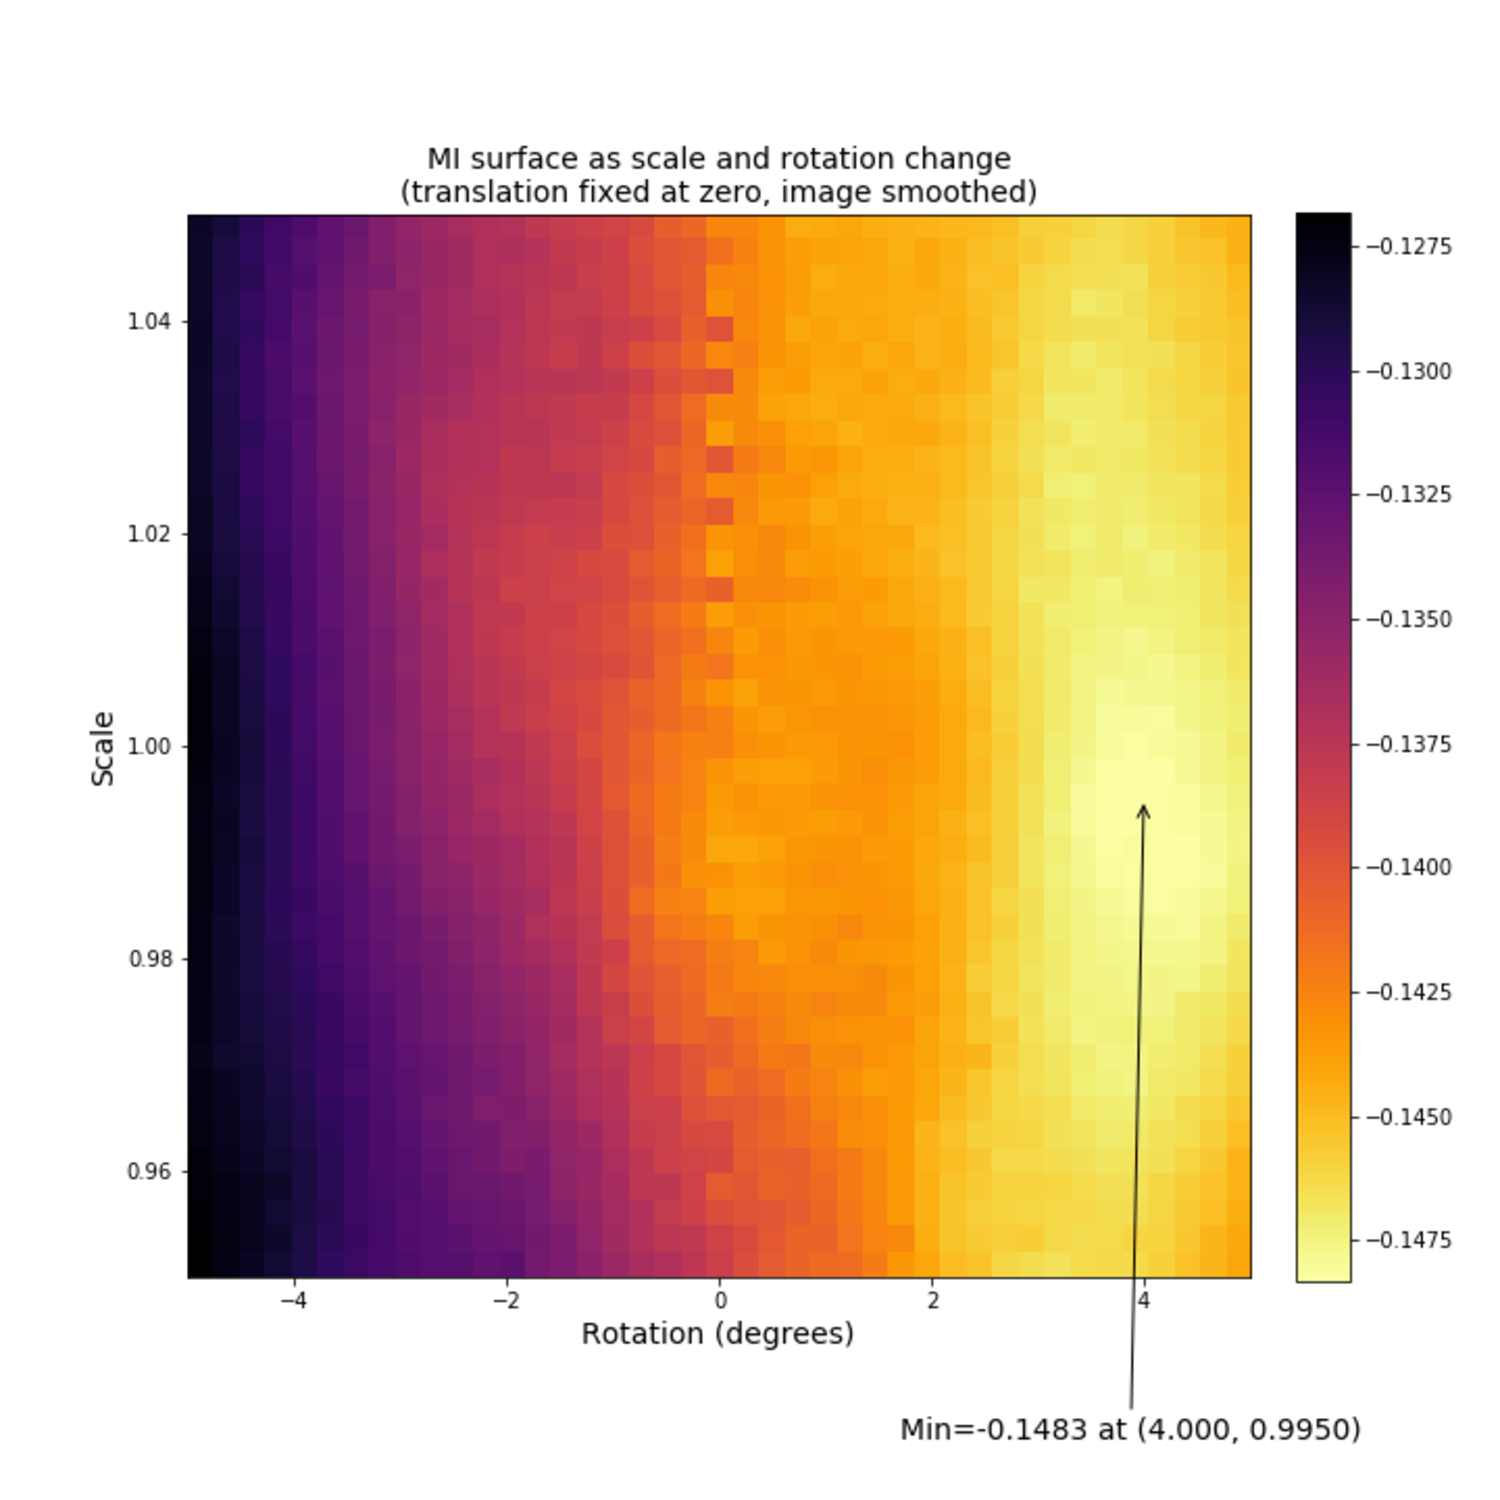
\includegraphics[width = 5 in]{MI_surf_blur3_qNone_im24_fig.pdf}} \\

\caption{Example Mutual Information surface for aligned pair of PCANet-based Structural Representations. Images (a) and (b) show the structural representations of an aligned pair of SHG and TPEF images (original images are shown in Figure \ref{fig:example_imageset_mpm} (a) and (d)). Image (c) shows the (negative) MI values over a grid of scale and rotation transforms. The translation is fixed at zero pixels. There is no clear peak for the scale parameter, although the highest value is found here at $\hat{T}_s = 0.995$, very close to the correct value ($T_s = 1$). The optimal MI position is found at a rotation of $\hat{T}_r = 4$ degrees instead of the true value $T_r = 0$.}
\label{fig:MIsurfacePSR}
\end{figure}

The structural representations also did not prove to be easy for mono-modal registration techniques such as MSE %and $\alpha$AMD
to align, as seen in the results. The optimal transform found using MSE on a grid gave a lower (better) MSE value than at the ground truth in the majority of cases, despite being more than 5 pixels away from the ground truth, so it was again not possible to improve the results with gradient descent.

\subsubsection{PCANet-based SR evaluation}
Although it is probable that somewhat clearer representations can be obtained through further tuning of the PSR model, it is unlikely (on the basis of results seen here) that the alignment of such representations, using mono-modal registration methods, would be any more accurate than alignment of the original image data, using multi-modal methods such as MI. Some examples of further tuning experiments with different hyperparameter values are shown in Appendix \ref{appendix:tuning}. 

It appears that the high-frequency nature of these images does not lend itself well to this form of structure extraction, even after smoothing.

\subsection{Alignment with Model 2: Discriminative Local Derivative Patterns}
\label{sec:model2_results}
In Model 2, the alignment minimizing the Hamming distance between the dLDPs for a pair of images is sought. Since a dLDP binary representation cannot be interpolated it is necessary to recalculate it at each candidate alignment. The (dis)similarity metric is then calculated as the mean Hamming distance, i.e.
\[
D(I_R, I_F, T) = \frac{1}{N} \sum_x R(I_R) \oplus R(T(I_F)),
\]
for candidate transform $T$ which, when applied to the representation $R(.)$ of the floating image $I_F$, leads to an overlap of $N$ pixels $x$ with the representation of the reference image $R(I_R)$. The symbol $\oplus$ denotes the binary XOR operator. The optimal alignment is the one which minimizes this measure. This was estimated using grid search and gradient descent.

\begin{figure}
\centering
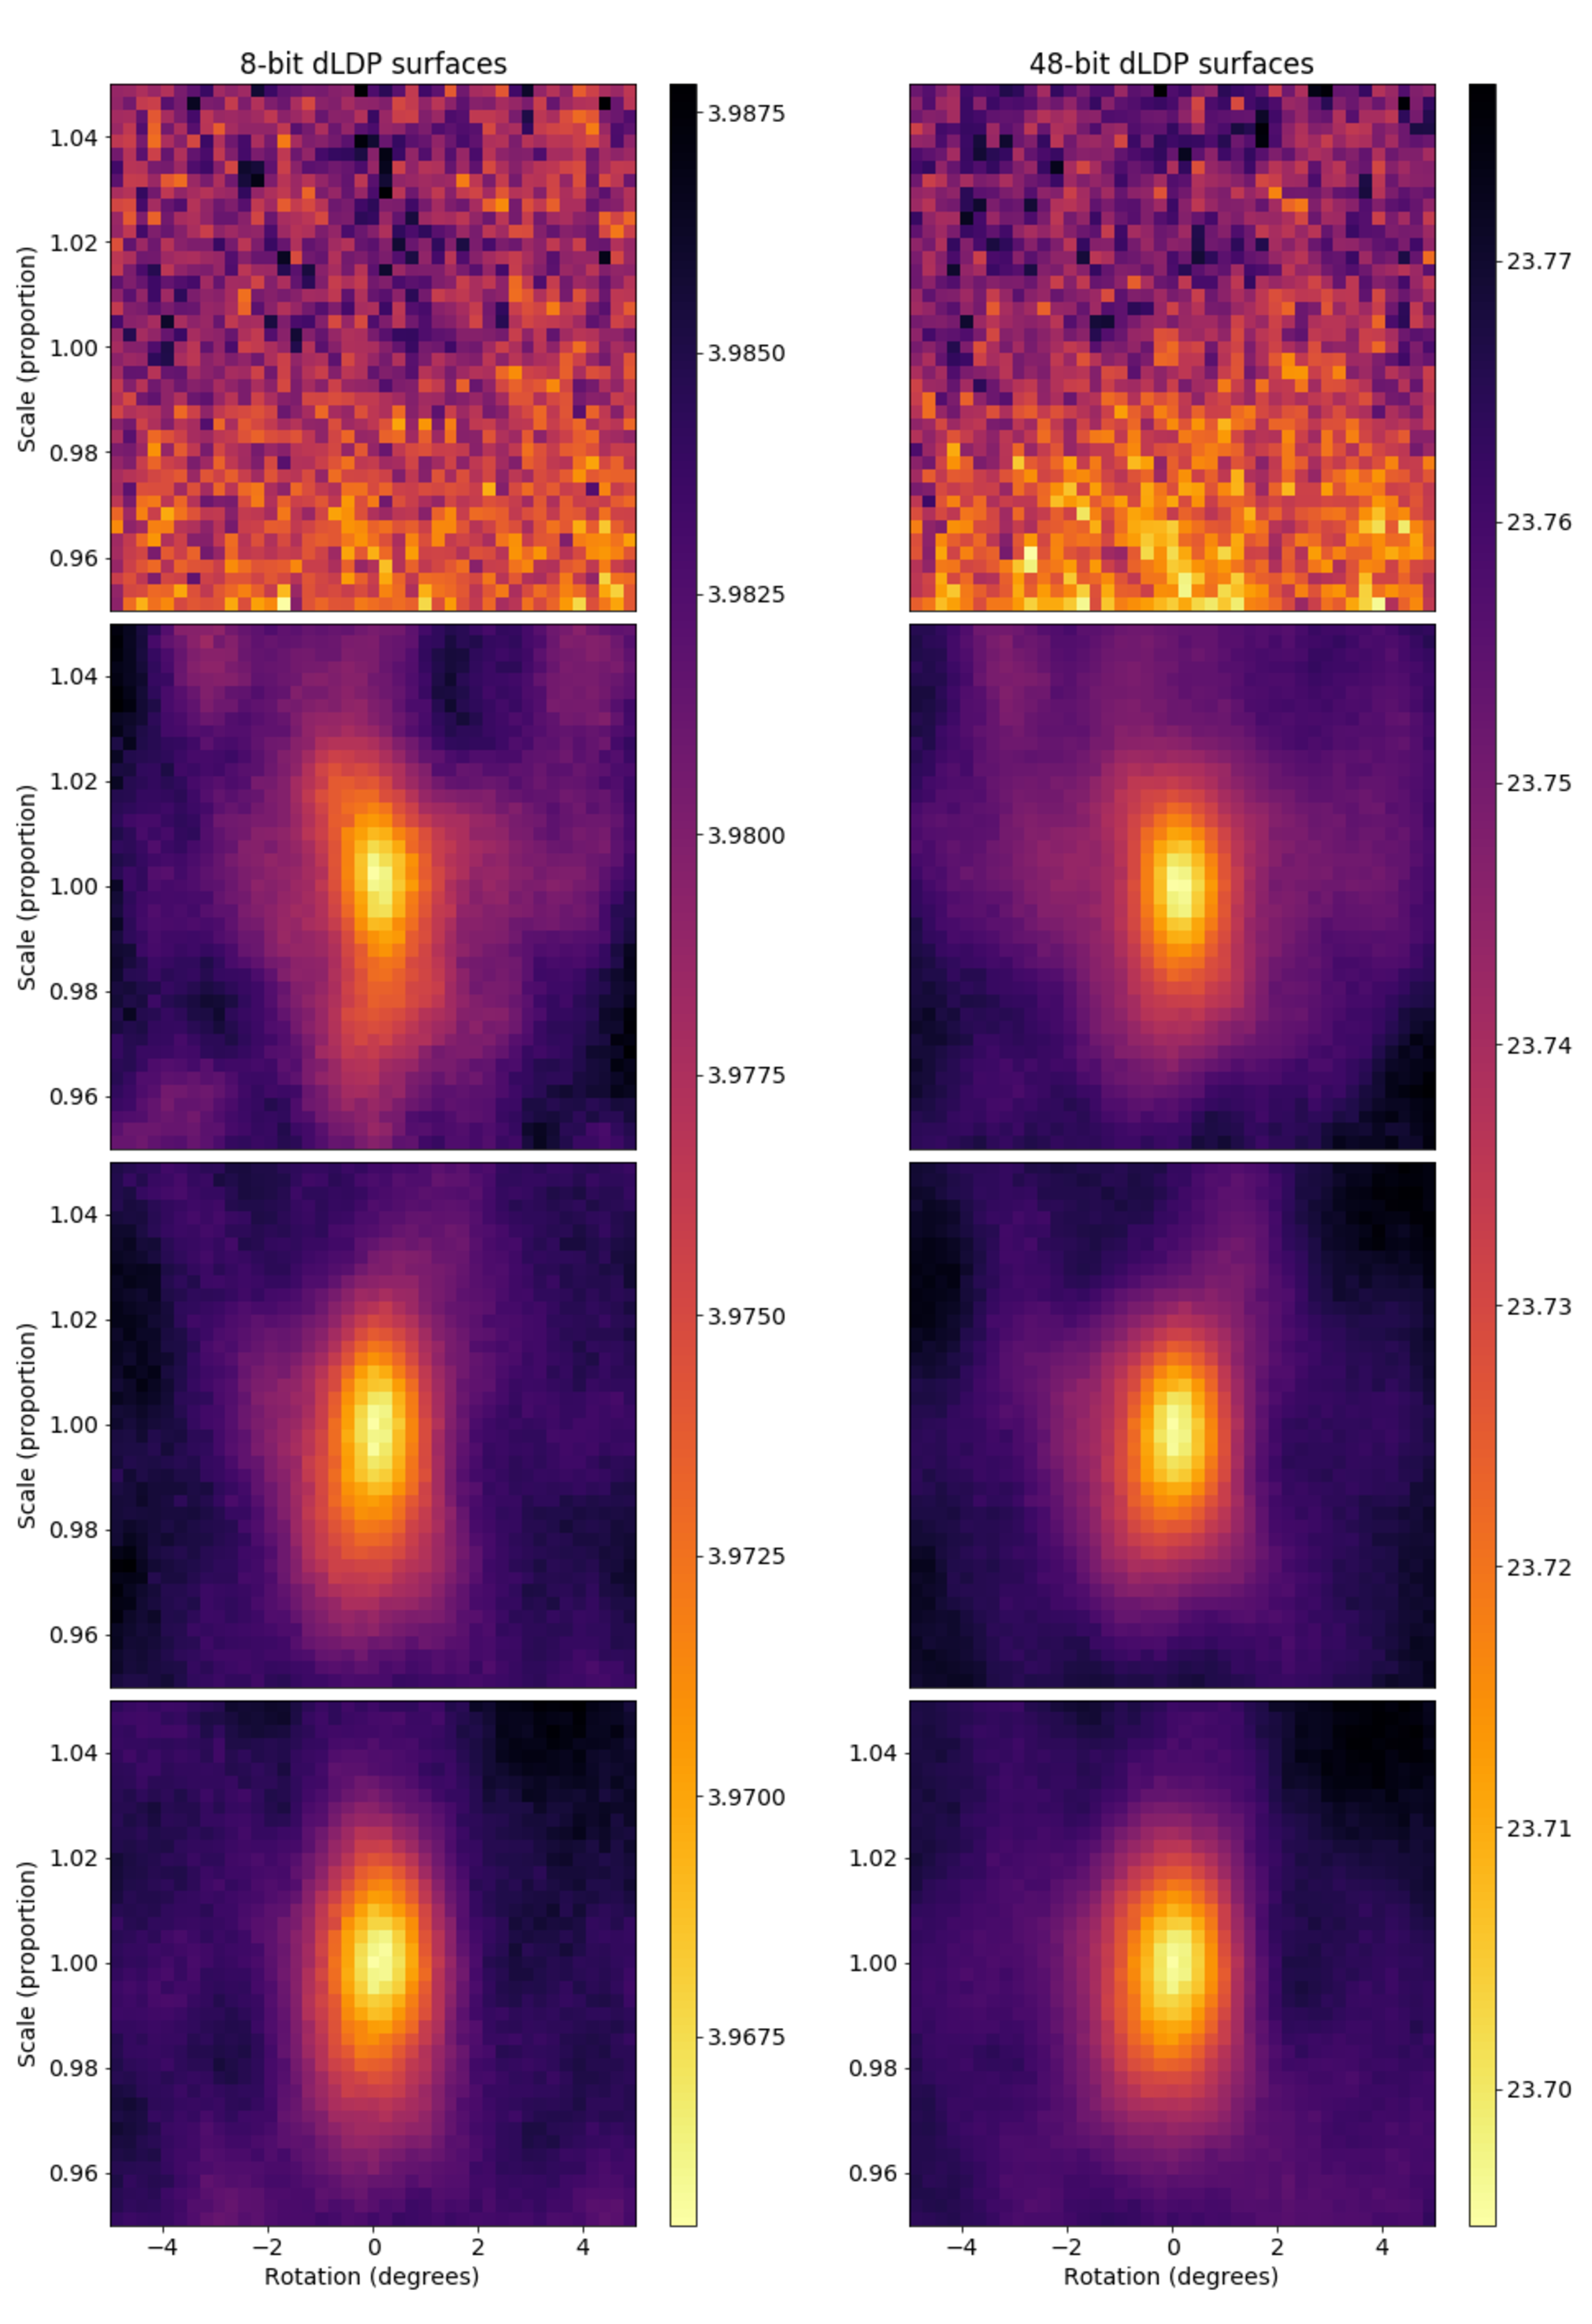
\includegraphics[width = 5.5 in]{bothgrids_bothblur_im24.pdf}

\caption{Example dLDP Hamming Distance surface for aligned pair of SHG and TPEF images as scale and rotation are changed. The first row shows the Hamming distance surfaces for the the 8-bit (left) and 48-bit (right) dLDP metrics for unsmoothed image pairs, as the scale and rotation of one image is adjusted. The second row shows the same surfaces for images smoothed with Gaussian filter ($\sigma=3.0$). In the third row, the images are smoothed and histogram equalization is applied. In the final row, after histogram equalization the images are quantized into 32 intensity bins.}
\label{fig:dLDPsurf}
\end{figure}

As described in Section \ref{sec:model2}, two different versions of the two-dimensional dLDP model were used: an 8-bit version, which encodes the commonality of direction of the $x$ and $y$ derivatives, and a 48-bit version encoding all unordered pairs of derivatives in the $0^{\circ}$, $45^{\circ}$, $90^{\circ}$, and $135^{\circ}$ directions. Both of these metrics give highly random results when applied to unsmoothed images, as shown in Figure \ref{fig:dLDPsurf} (first row). However, if the images are first smoothed with a Gaussian filter ($\sigma=3$), a more promising result can be seen (Figure \ref{fig:dLDPsurf}, second row). Histogram equalization, with or without quantization into 32 intensity bins (Figure \ref{fig:dLDPsurf}, fourth and third rows), had a less dramatic effect, but also improved results somewhat. The quantization had little effect and was not pursued further.

The results of using Model 2 to align smoothed SHG and TPEF images are shown in Table \ref{tab:dLDPresults}. With 8-bit dLDPs, the optimum transform found using a grid search usually had a lower dLDP Hamming distance than at the ground truth, even though in many cases the registration was very far from the correct alignment. With the 48-bit version, many more registrations were successful (52\% compared to 20\% for 8-bit), demonstrating that the minimum Hamming distance with this measure is more often found close to the ground truth transform than for the 8-bit version. The remainder of tests were therefore performed using the 48-bit dLDP.

Tests using gradient descent had little success either when starting the search from the identity transform or when adding an additional 20 random starting points. In a minority of cases an extreme transform, where few of the original pixels of the floating image were used in the comparison, was found to give a very low Hamming distance. This could be overcome through using a penalty term in the optimization process. However, even when an extreme transform giving an unwanted high similarity measure was \textbf{not} found, in most cases the registration was still unsuccessful.

\begin{table}
\centering

\begin{tabular}{|p{1.2in}|p{0.4in}|p{1.05in}|p{0.6in}|p{0.9in}|}
\hline
%\centering
\textbf{dLDP Alignment Method} & \textbf{dLDP bits} & \textbf{Pre-processing} & \textbf{Median error $E$ (pixels)} & \textbf{Successful registrations (\%)} \\
\hline
\hline
1a. Grid search & 8 & Smoothing & 21.57 & 20  \\ %PartIII_test1.3_8bit
\hline
1b. Grid search & 8 & Smoothing and Histogram Equalization & 2.92 & 76  \\ %PartVII_test1.3_8bit
\hline
2a. Grid search & 48 & Smoothing & 4.33 & 52  \\ %PartIII_test1.3_48bit
\hline
2b. Grid search & 48 & Smoothing and Histogram Equalization & 2.61 & 96  \\ %PartVII_test1.3_48bit
\hline
%3. Gradient descent (from identity transform) & 48 & Smoothing & 23.03  & 0 \\  %PartIII_test3.10_48bit
3. Gradient descent (from identity transform) & 48 & Smoothing and Histogram Equalization & 21.53  & 8 \\  %PartVII_test3.3_48bit
\hline
4. Gradient descent (multi-start) & 48 & Smoothing and Histogram Equalization & 6.28  & 48 \\  %PartVII_test5.3_48bit
\hline
\textbf{5. Gradient descent (from result of 2b)} & \textbf{48} & \textbf{Smoothing and Histogram Equalization} & \textbf{2.08}  & \textbf{96} \\  %PartVII_test6.3_48bit
%5. Gradient descent (from result of 2a) & 48 & Smoothing & 4.33  & 52 \\  %PartIII_test6.10_48bit
\hline
\end{tabular}
\caption{Results of using 8-bit and 48-bit dLDP structural representations to align SHG and TPEF images, with different optimisation strategies and data pre-processing steps. Histogram equalization significantly improved the results for both 8-bit and 48-bit descriptors.}
\label{tab:dLDPresults}
\end{table}



\subsubsection{dLDP Evaluation}
As found with Mutual Information and with PCANet-based Structural Representations, the high-frequency detail in the MPM images makes them difficult to align. Smoothing is essential for this method, and histogram equalization also had a beneficial effect. With both of these pre-processing steps, a high success rate was obtained when registering images with the 48-bit dLDP descriptor. Attempts to find the optimum transform using gradient descent were once again unsuccessful but further experiments and tuning might provide improved results, based on the apparently smooth surfaces of descriptor values (although this may be misleading as it is only readily depicted in 2 out of the 4 parameter dimensions) seen in Figure \ref{fig:dLDPsurf}.

\section{Task 2: Alignment of Brightfield and MPM images}
\label{sec:eval_bf_mpm}

It is clear from the above results that the alignment of SHG with TPEF images is a challenging task, because of the high-frequency nature of these images and the different biological structures visible in each modality. Brightfield images are, to the eye, even more dissimilar to the MPM images than the MPM images are to each other. But the registration of brightfield images with MPM images is needed in order to assist pathologists with diagnosis of clinical samples such as the ones used in this study. The above methods were therefore evaluated on pre-aligned pairs of brightfield and MPM images, to see whether the methods could verify the ground truth.

Based on results from Task 1, three experiments were conducted:
\begin{enumerate}
    \item Mutual Information grid search on original images.
    \item Mutual Information grid search on PCANet-based structural representations of images. The networks were trained with $c_1=0.05$, $_2=0.1$ (brightfield) and $c_1=0.025$, $c_2=0.1$ (MPM), using smoothed versions of the original images. The resulting PSRs were also smoothed.
    \item 48-bit dLDP Hamming distance grid search. The images were smoothed and histogram-equalized.
\end{enumerate}

Although the images have been manually aligned, brightfield and MPM images are captured from different (adjacent) tissue slices (see Section \ref{sec:data}). This means that although closely related, there are slight differences between the shapes and relative positions of the structures in the brightfield image as compared to the MPM image. This would be expected to further increase the difficulty of registration, and this is borne out by the results shown in Table \ref{tab:task2results}.

\begin{table}
\centering
%\begin{tabular}{|p{1.2in}|p{1.05in}|p{0.6in}|p{0.9in}|}
\begin{tabular}{|p{1.2in}|p{1.05in}|p{0.6in}|p{0.9in}|p{0.9in}|}
\hline
\textbf{Registration Method} & \textbf{Pre-processing} & \textbf{Median error $E$ (px)} & \textbf{Successful registrations (\%)} & \textbf{Computation time} \\
\hline
\hline
1. NMI grid search & None & 24.7 & 0 & 29 mins \\
\hline
2. PSR with NMI grid search & Smoothing of original images and PSRs & 21.43 & 8 & 31 mins \\
\hline
3. dLDP 48-bit grid search & Smoothing and Histogram Equalization & 20.76 & 0 & 49 mins \\
\hline
\end{tabular}
\caption{Results for Task 2: Alignment of Brightfield and MPM images. 25 pairs of pre-aligned images, with a known transform applied to one image in each pair, were aligned using each method. The median error $E$ is given for each method, along with the proportion of registrations which were successful.}
\label{tab:task2results}
\end{table}

\begin{figure}
\centering
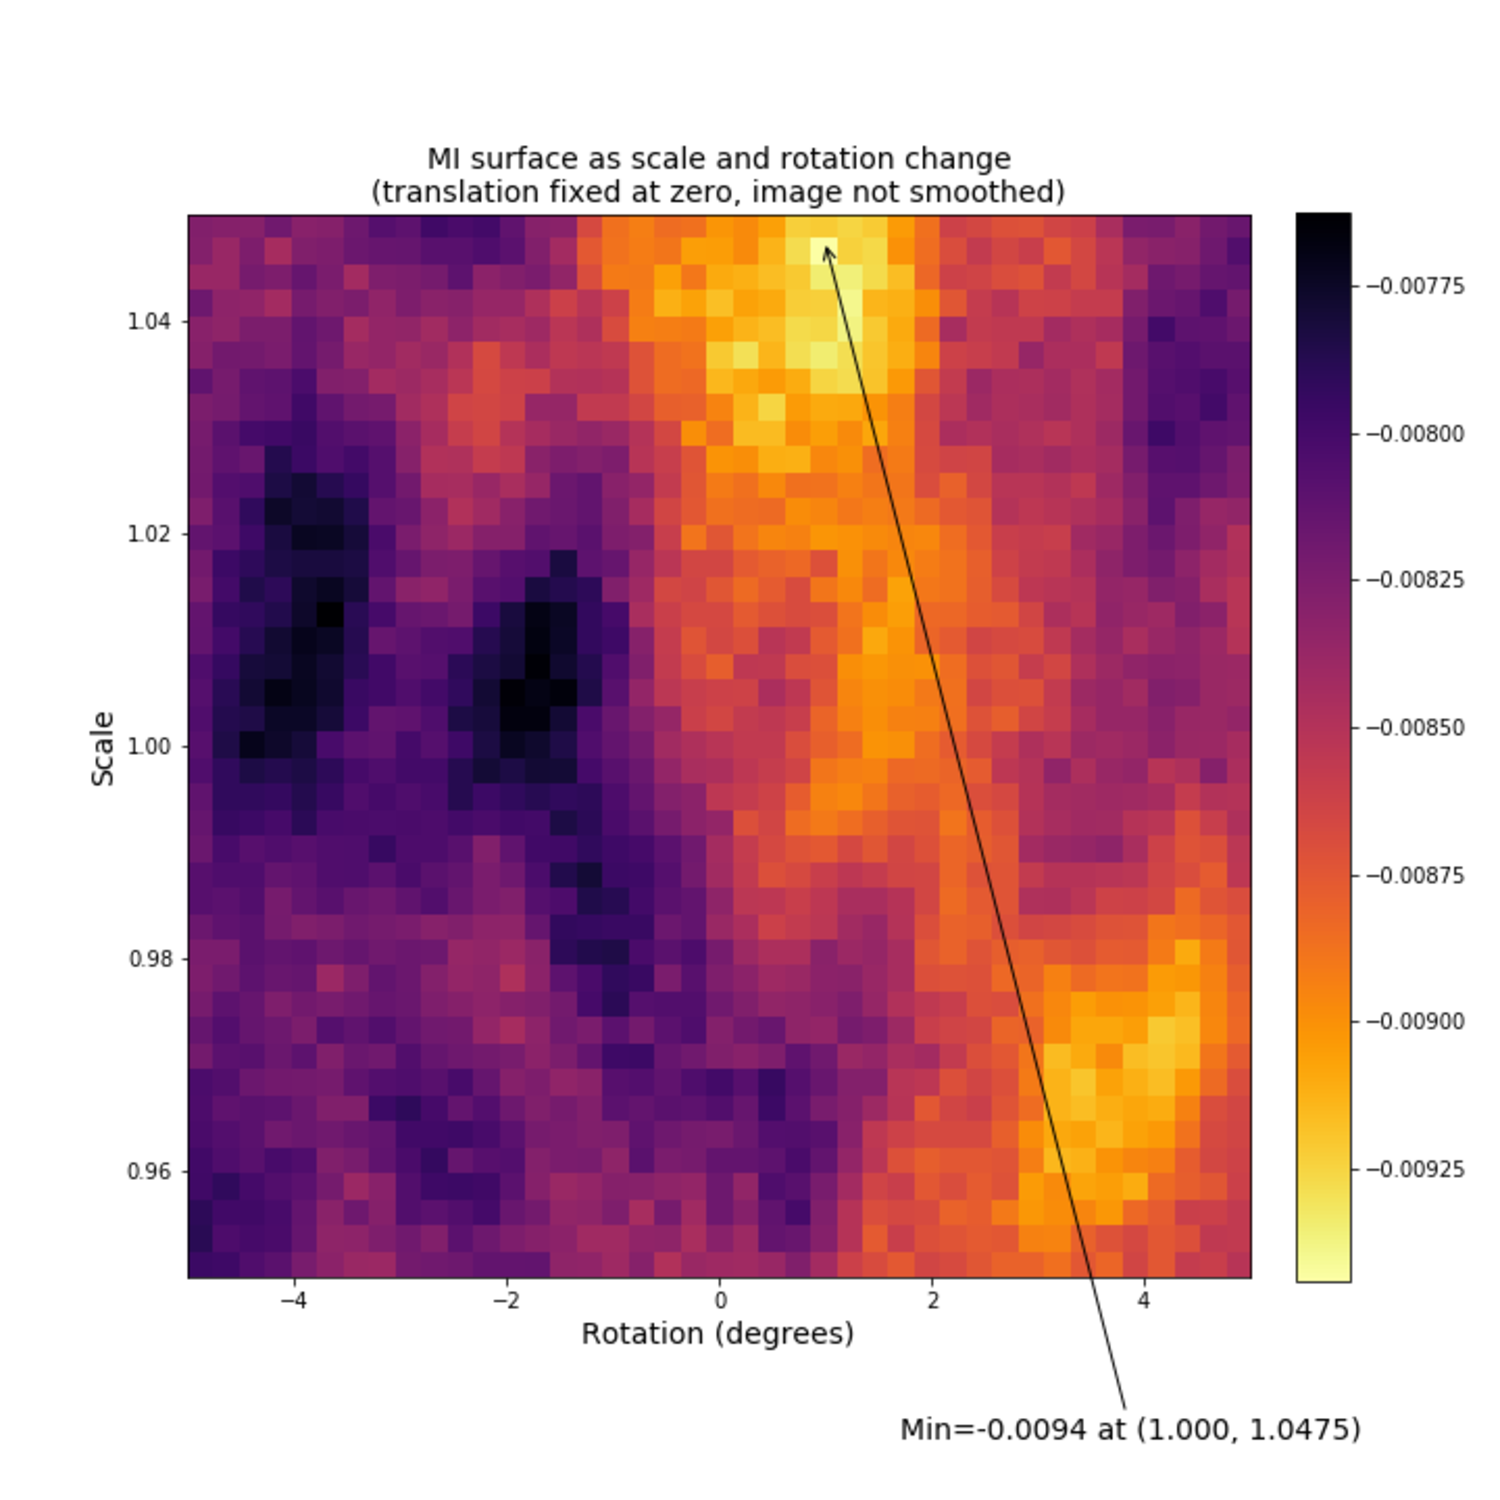
\includegraphics[width = 5 in]{MI_blur0_qNone_im11_fig.pdf}

\caption{Example Mutual Information surface for manually aligned brightfield and MPM images. The (negative) NMI values are calculated over a grid of scale and rotation transforms. The translation is fixed at zero pixels.
The peak value for the metric is found here at ($\hat{T}_s = 1.0475$ $\hat{T}_r = 1.00$), giving $E=22.2$, but several other local optima can be seen.
}
\label{fig:bf_mpm_surf}
\end{figure}

In many cases in all three experiments (100\% for experiment 1, 92\% experiment 2, 40 \% experiment 3), the optimum transform found on the grid had a higher similarity metric value than that at the ground truth position (e.g. NMI metric values shown in Figure \ref{fig:bf_mpm_surf}). This indicates that it would not be possible, with these methods under the tested conditions, to find the correct registration.

%\section{Evaluation of ground truth}
%\label{sec:ground_truth}
%In order to evaluate the results of different methods, a reliable ground truth is required as a baseline for comparison. As described above in Chapter \ref{sec:data}, 400 regions of interest were imaged using multiphoton microscopy (MPM). The approximate location of each MPM region was marked on a larger brightfield image, showing a neighbouring slice within the same sample of skin tissue. These marked regions, described here as the 'given ground truth' (GGT), were manually marked by hand and in some cases could be seen to be somewhat distant from the exact location of the MPM image, perhaps as much as 50 pixels. It was therefore necessary to seek a more exact location, a 'refined ground truth' (RGT).
%

%\chapter{Discussion and Future Work}
%\textit{Todo: What was good, what was bad about this project. What was there not time for. What factors were and were not taken into account that might affect the results. How can it be extended, improved, generalized.}

\chapter{Conclusions}
Many alternative methods have been proposed for extracting structure from multi-modal images, alongside algorithms for using such structure to register images. The performance of two such models on the registration of Second Harmonic Generation Microscopy with Two Photon Excitation Fluorescence Microscopy images has been evaluated in this study, and results show that neither technique is effective on this particular type of data. Various types of pre-processing of the image data might improve their performance, by filtering out the high-frequency signal in order to highlight the underlying structures. In this study, smoothed images were tested as well as the original images, which improved the continuity of the evaluated metrics but did not give greatly improved results overall. In addition, experiments were repeated with histogram equalization, a method of increasing the contrast of an image. This led to improved results for the dLDP method in particular.

Efforts here have focused on accuracy rather than efficiency of methods but this should not be overlooked. Processing time, and to a lesser extent training time, is an important factor in developing methods that can be used in live clinical applications. The alignments attempted in this study were extremely challenging and a grid search over a range of parameters was found to be the only effective way to find an optimal alignment. This is highly computationally expensive, requiring over 15 000 metric calculations even for a coarse grid of 11 steps in each of 4 dimensions. Times reported in Tables \ref{tab:task1results} and \ref{tab:task2results} are based on Python implementations which could undoubtedly be further optimised, and this is perhaps true of the dLDP method more than the other methods, where timings are generally dominated by a Mutual Information function implemented in the Python library scikit-learn\footnote{https://scikit-learn.org/}, likely to be quite efficient. For this reason, the timings reported are not fully comparable between the methods.

The real task required for patient diagnosis is the alignment of MPM images with brightfield images, and this proved even more challenging than the registration of TPEF and SHG images. There is very little low-level correspondence between the images, partly due to the different features imaged by the different modalities, and partly because the images are taken of two different slices (stained and unstained) from the sample provided. Although the correct registration can be identified by eye from the larger structures in the images, there tend to be differences in the extent and outline even of these. None of the methods tested in this study was effective in the registration of MPM and brightfield images.

\section{Acknowledgements}
Heartfelt thanks to my supervisors Johan Öfverstedt and Joakim Lindblad, and my reviewer Nata\v sa Sladoje, for all their excellent suggestions, patience, and support. Many thanks also to the rest of the Methods in Image Data Analysis (MIDA) group at Uppsala University's Division of Visual Information and Interaction, for help and feedback. All mistakes are my own.

\bibliography{bibliography}{}

\appendix
\chapter{Tuning Model 1: further details}
\label{appendix:tuning}
As described in Section \ref{sec:evalPSR}, different combinations of the model parameters $c_1$ and $c_2$ were tested for each modality of interest. The values tested were 0.01, 0.05, 0.1, 0.2, and 0.5. Note that the recommended values for MRI images, given in \cite{zhu2018pcanet}, were $c_1=0.8$ and $c_2=0.6$. However, for both SHG and TPEF images, high values of $c_1$ and $c_2$ give very pale images in which little or no structure is visible, even after normalization.

An example PSR for each combination is shown in Figures \ref{fig:tpef_tuning} (TPEF) and \ref{fig:shg_tuning} (SHG). This comparison shows that there is no value of the hyperparameters $(c_1, c_2)$, which gives a structural representation of a TPEF image that appears similar to any of the structural representations shown in Figure \ref{fig:shg_tuning} of the corresponding SHG image. The dark band that appears in the middle of the SHG image is very faint or invisible in the TPEF images, which instead feature a dark region that starts immediately below this band.

\begin{figure}
\centering
\subfloat[]{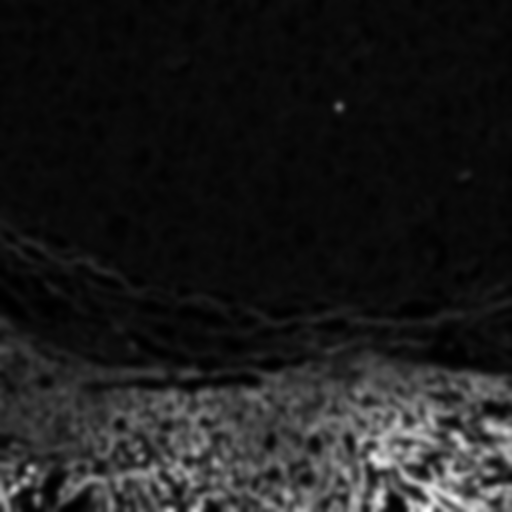
\includegraphics[width=2in]{TPEF_148185_11_blur3_norm.png}} \\
\subfloat[]{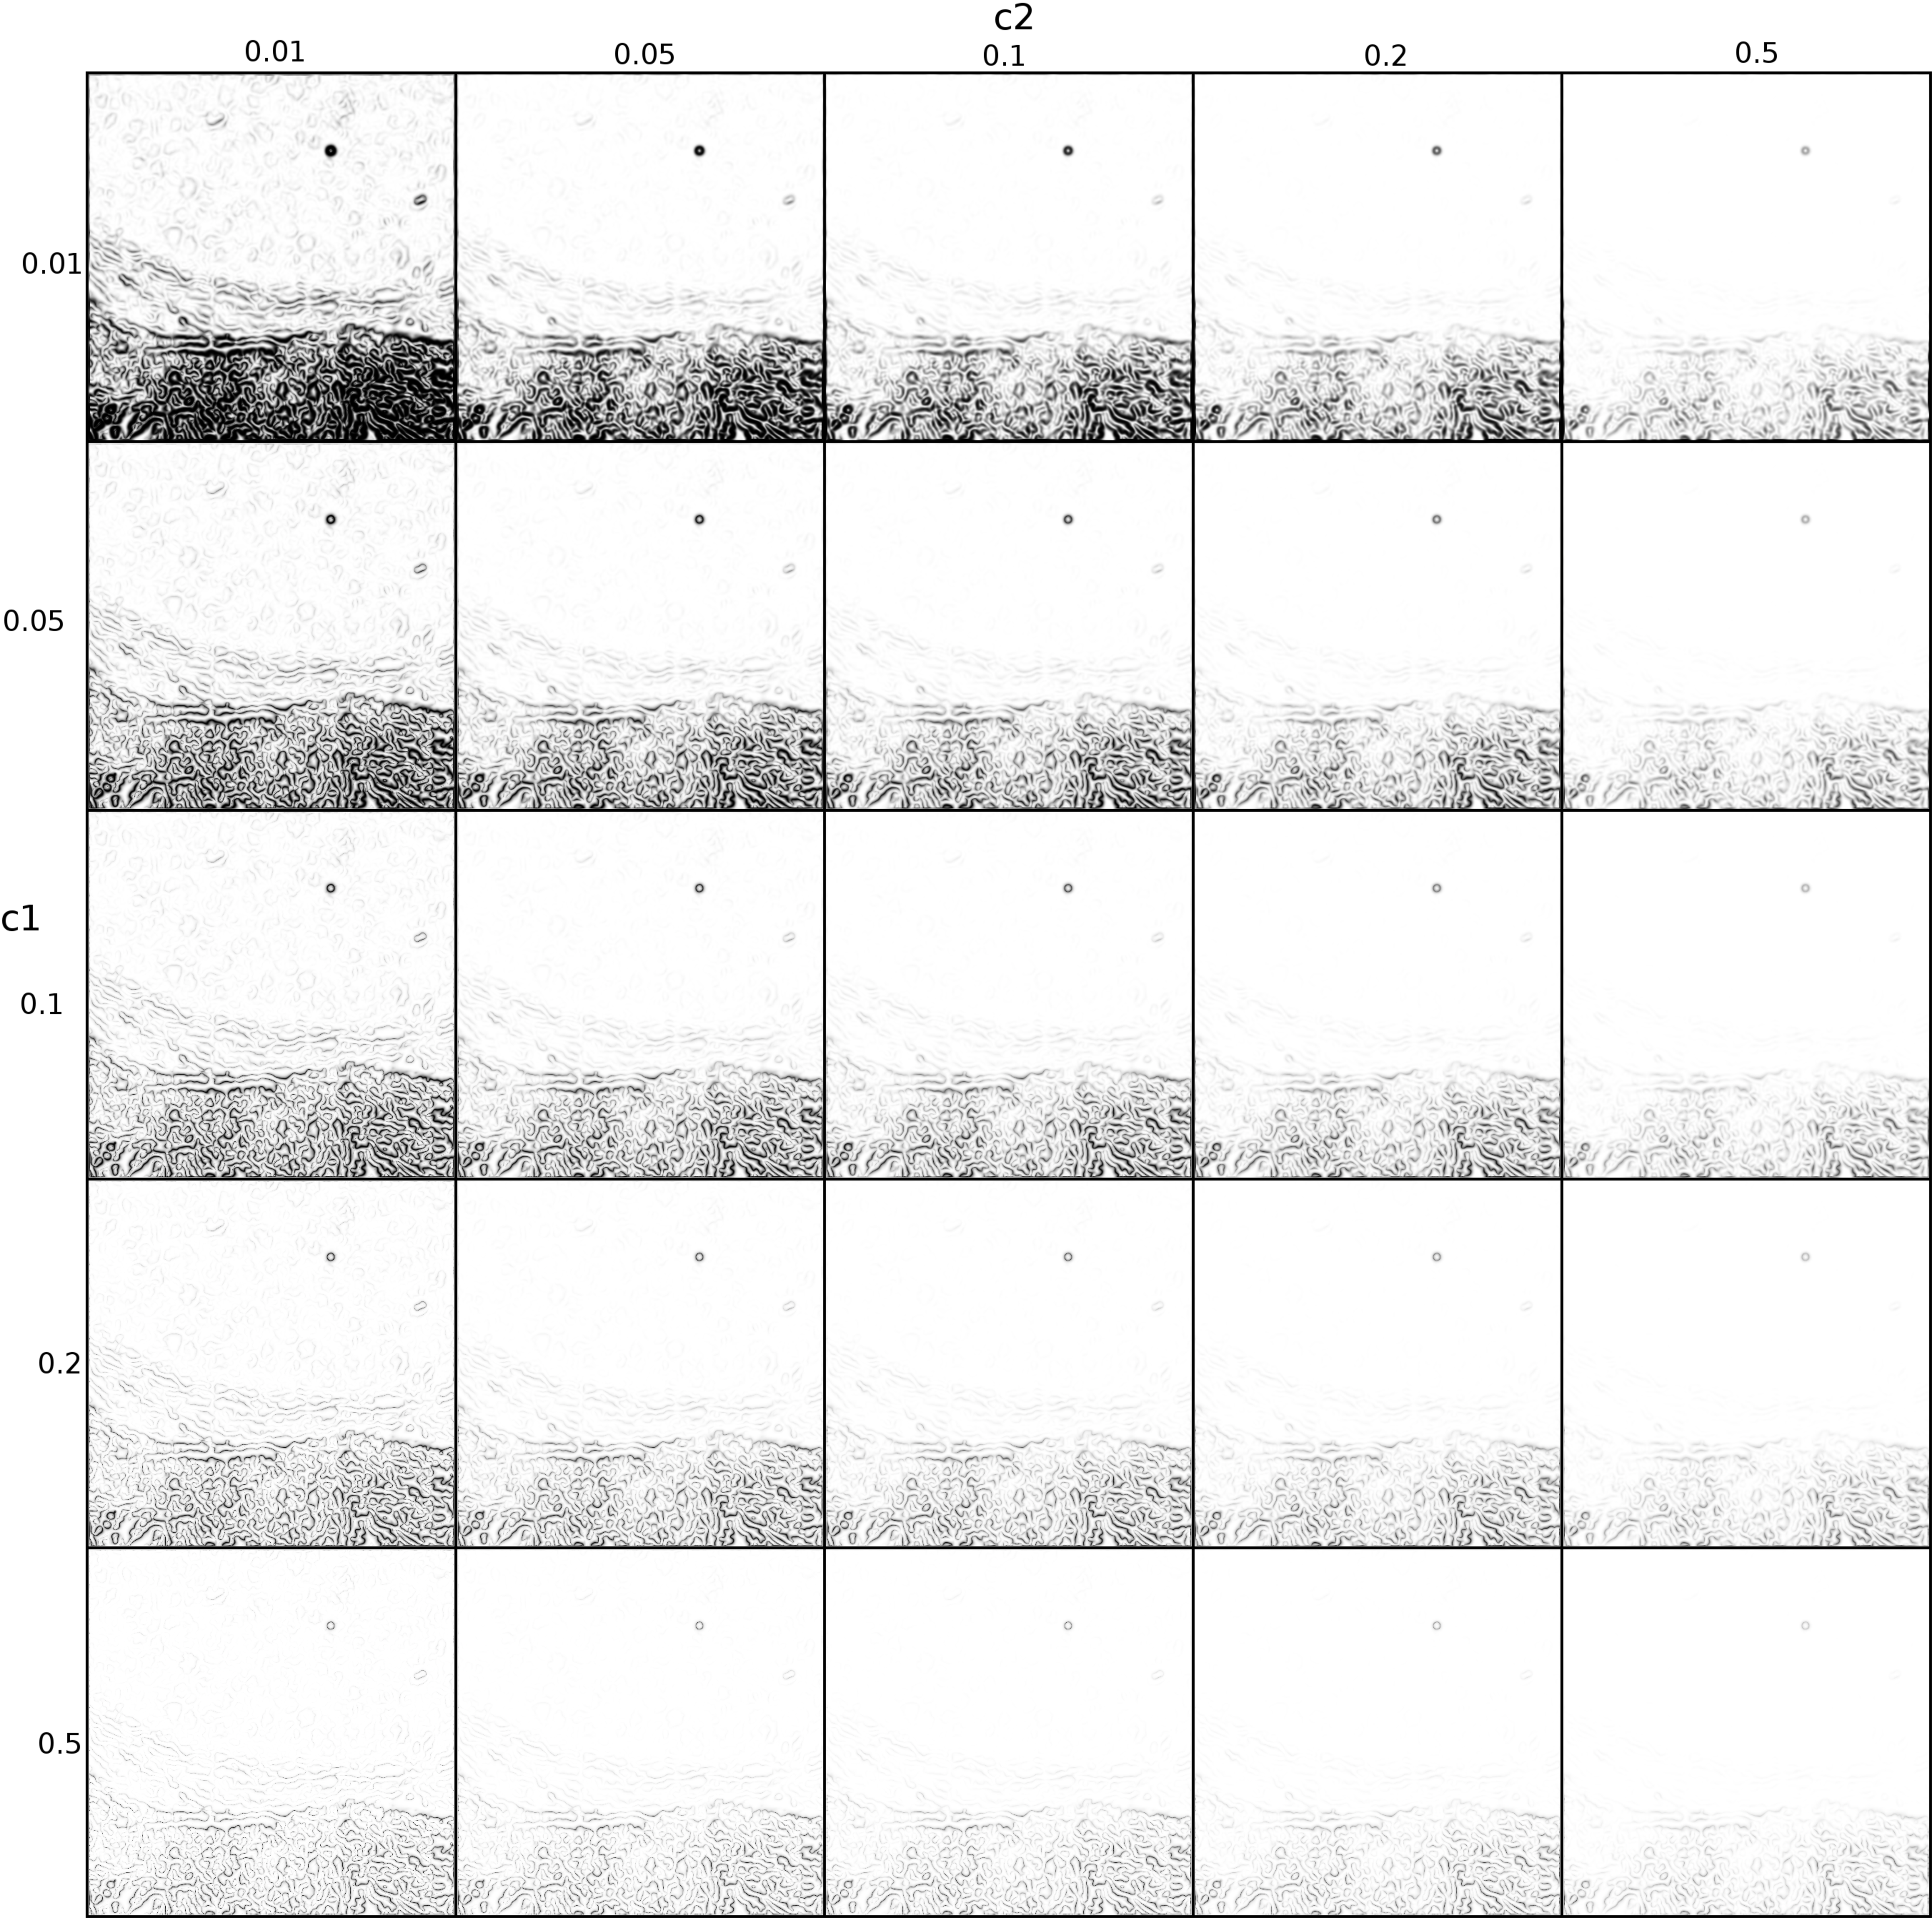
\includegraphics[width=5.8in]{TPEF_blur3_ds1_grid.pdf}}

\caption{Results of training Model 1 using TPEF images, with various combinations of $c_1$ and $c_2$. Image (a) is the original TPEF image for slide 148185 region 11, with Gaussian smoothing ($\sigma=3$). Image (b) shows the output structural representations for each parameter combination.}
\label{fig:tpef_tuning}
\end{figure}

\begin{figure}
\centering
\subfloat[]{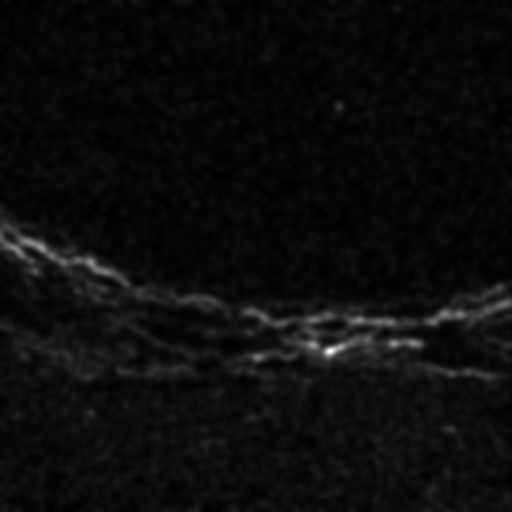
\includegraphics[width=2in]{SHG_148185_11_blur3_norm.png}} \\
\subfloat[]{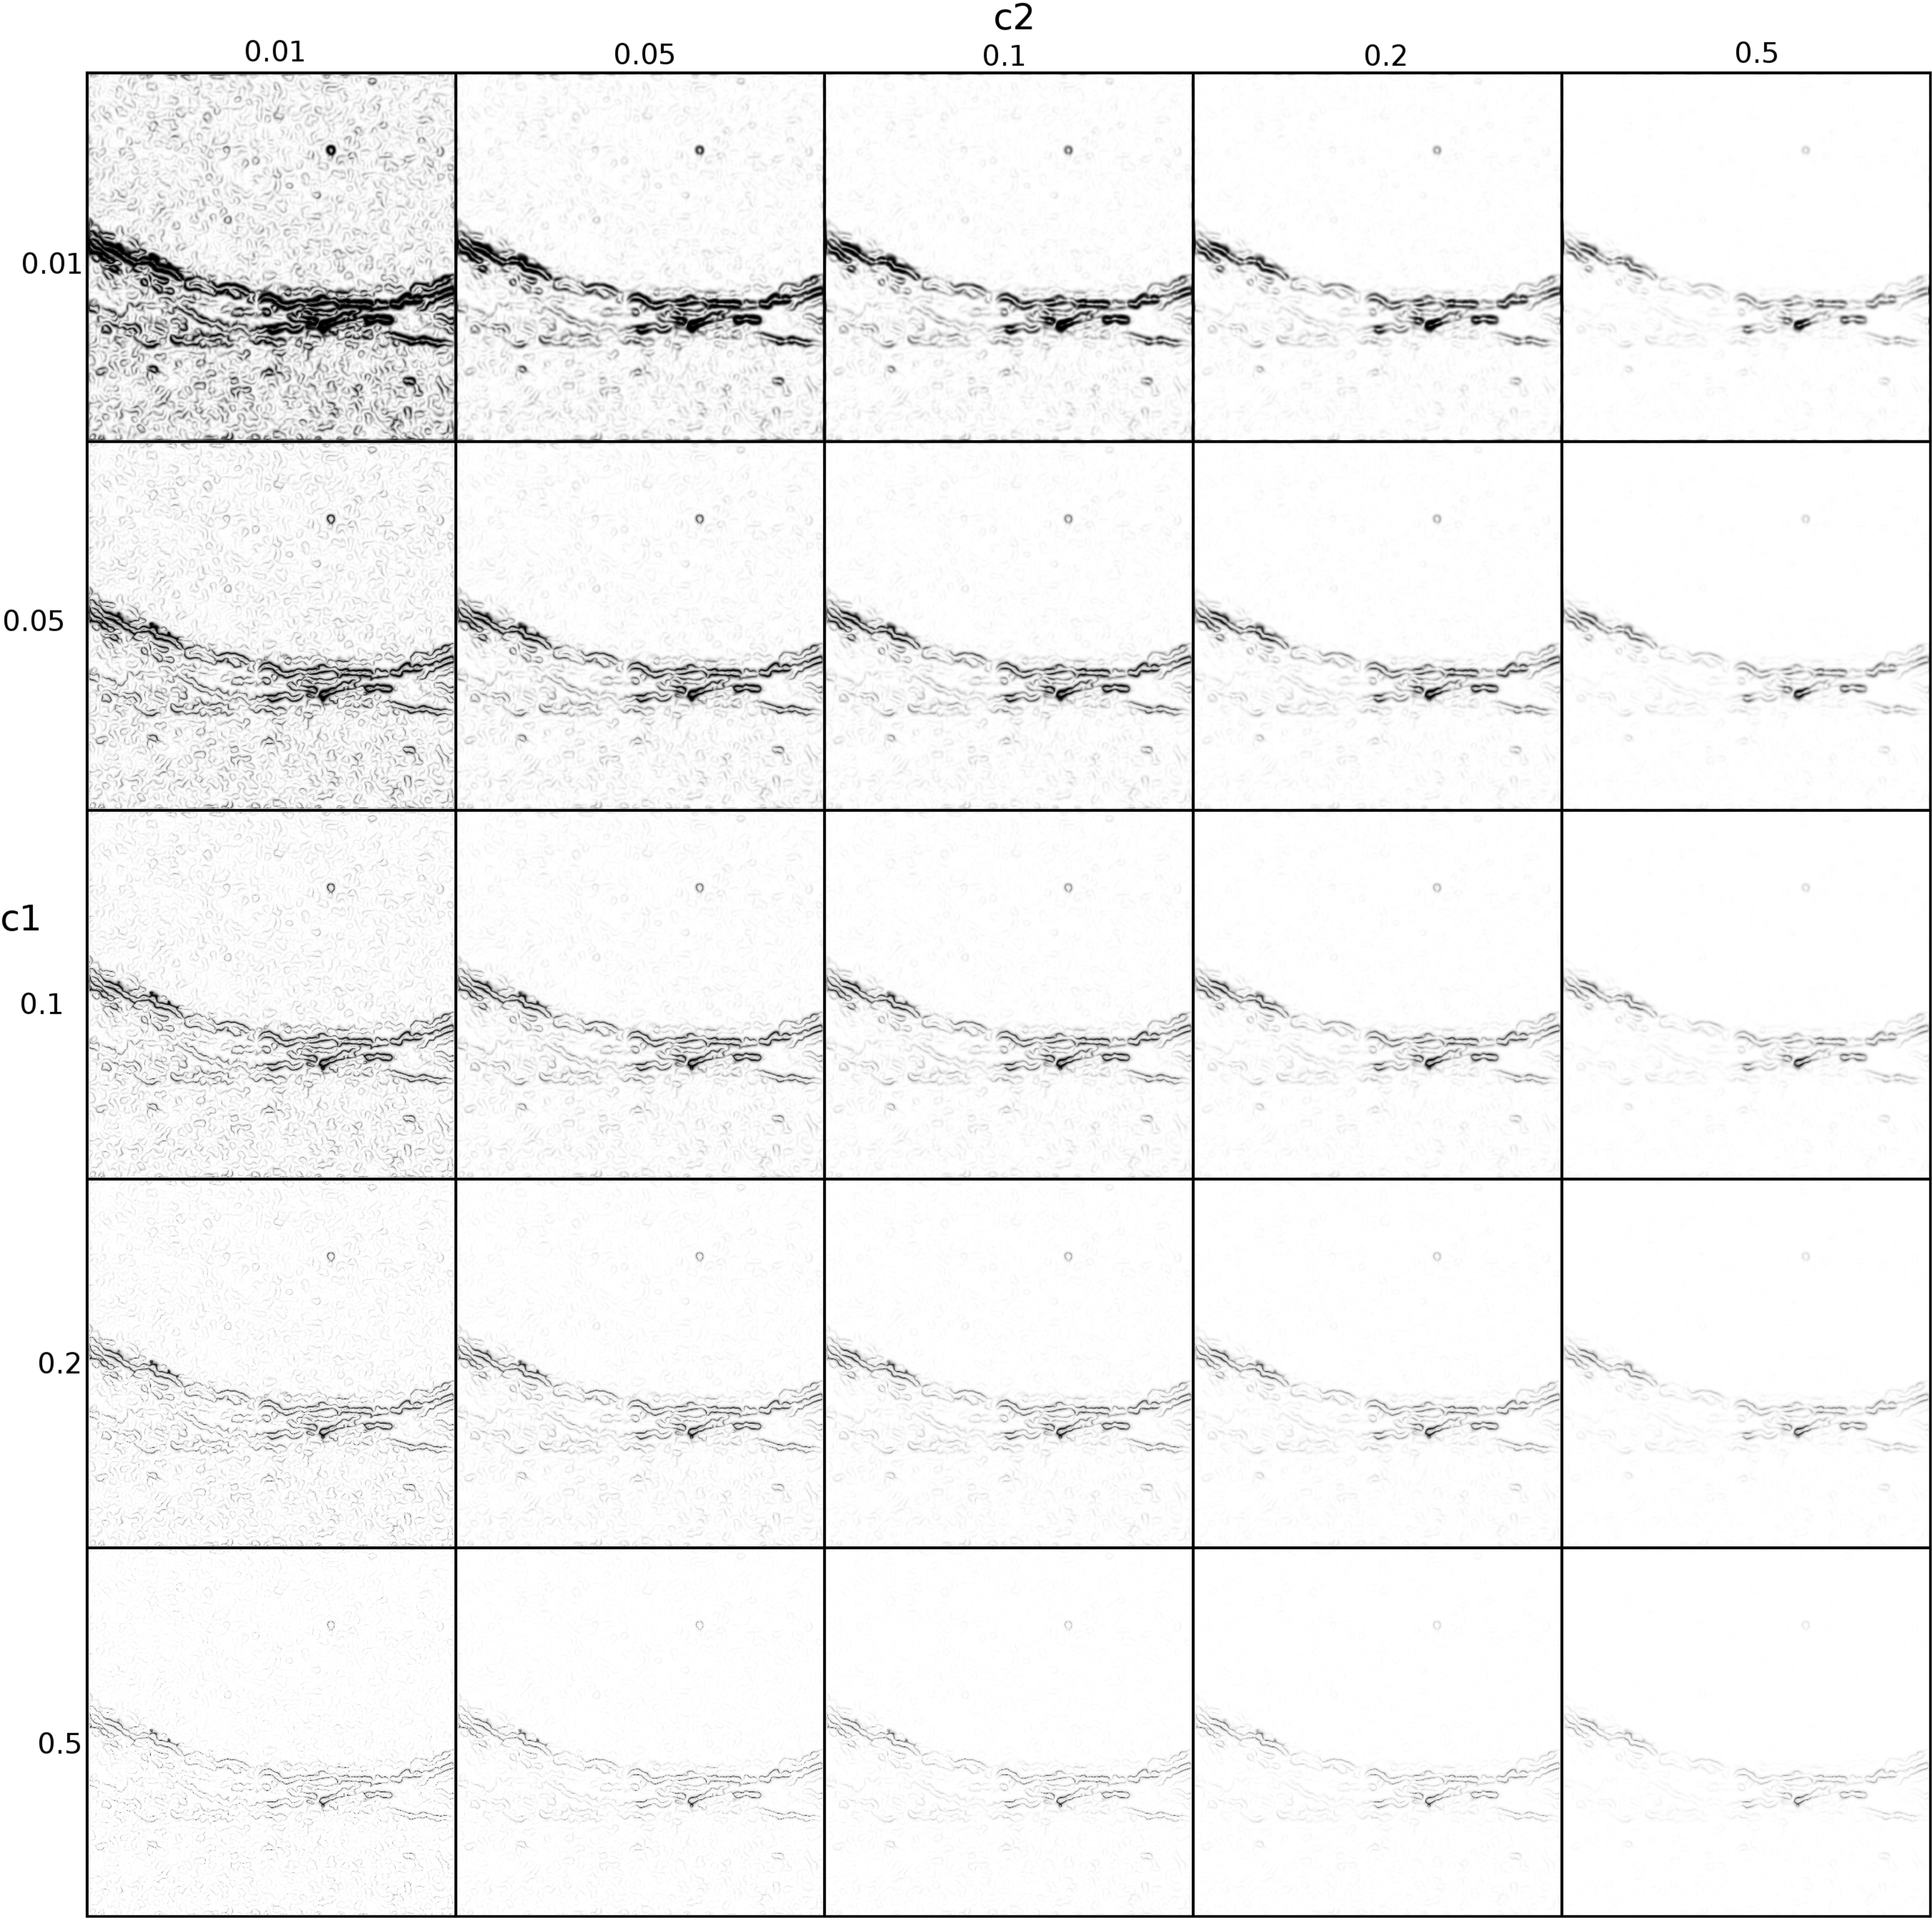
\includegraphics[width=5.8in]{SHG_blur3_ds1_grid.pdf}}
\caption{Results of training Model 1 using SHG images, with various combinations of $c_1$ and $c_2$. Image (a) is the original SHG image for slide 148185 region 11, with Gaussian smoothing ($\sigma=3$). Image (b) shows the output structural representations for each parameter combination.}
\label{fig:shg_tuning}
\end{figure}

Further experiments were undertaken with different filter sizes and downsampling schemes, without success.


\end{document}
